\documentclass[titlepage,a4paper,12pt]{book}

\usepackage[utf8]{inputenc}
\usepackage[catalan]{babel}
\usepackage{graphicx}
\usepackage{marvosym}
\usepackage{verbatim}
\usepackage{amssymb, amsmath} 
\usepackage{listings}
\usepackage{textcomp}
\usepackage{url}
\usepackage[]{color}


\begin{document}

\thispagestyle{empty}
%PAGINA3
\rule{160mm}{0.20mm}\\
\textbf{DADES DEL PROJECTE}\\
\\
\textit{Títol del Projecte:} Algoritmes genètics aplicats a ciències de la vida\\
\\
\\
\textit{Nom de l'estudiant:}Raimon Grau Cuscó\\
\\
\textit{Titulació:} Enginyeria Informàtica\\
\\
\textit{Crèdits:} 37.50 \\
\\
\textit{Director/Ponent:} Ignasi Belda Reig / Jordi Delgado Pin\\
\\
\textit{Departament:} Llenguatges i Sistemes Informàtics\\
\\
\\
\rule{160mm}{0.20mm}\\
\textbf{MEMBRES DEL TRIBUNAL}\textit{(nom i signatura)}\\
\\
\textit{President:} Ricard Gavaldà Mestre .\\
\\
\\
\textit{Vocal:} Manel Canales Gabriel.\\
\\
\\
\textit{Secretari:} Jordi Delgado Pin.\\
\\
\\
\\
\rule{160mm}{0.20mm}\\
\textbf{QUALIFICACIÓ}\\
\\
\textit{Qualificació numèrica:}\\
\textit{Qualificació descriptiva:}\\
\\
\textit{Data:}
\\
\\
\rule{160mm}{0.20mm}\\
%end pagina3
\newpage{\pagestyle{empty}\cleardoublepage}
%PORTADA AMB FOTOS I TAL SINÓ FORA
\begin{titlepage}
\begin{center}
{\Huge Algorismes genètics aplicats a ciències de la vida}\\[2cm]
{\Large  Raimon Grau Cuscó }\\[5cm]

	%\begin{figure}[h]
	%\begin{center}
	%%\includegraphics[width=4in]{img/ip.eps}
	%\end{center}
	%\end{figure}

	%\begin{figure}[h]
	%\begin{center}
	%%\includegraphics[width=3in]{img/bsc.eps}
	%%\includegraphics[width=1in]{img/gridSS.eps}
	%\end{center}
	%\end{figure}
\end{center}
\end{titlepage}

\newpage{\pagestyle{empty}\cleardoublepage}

\pagenumbering{roman}

%INICIEM
\tableofcontents

\newpage{\pagestyle{empty}\cleardoublepage}

%Introducció
\section{L’optimització numèrica} Gran part dels problemes a resoldre que es
presenten en els diversos camps de la ciència i la enginyeria es poden abstreure
com a problemes d’optimització numèrica: des de problemes de disseny industrial,
com per exemple l’optimització de peces de motors de combustió, fins al
modelatge de patrons de comportament biològic de models animals
d’experimentació. Sovint, aquests problemes presenten una sèrie de
característiques comunes que els fa complexos i difícils de tractar amb mètodes
d’optimització ‘‘clàssics´´ com poden ser tècniques com en \emph{backtracking},
\emph{branch and bound} o el \emph{simulated annealing}. Aquestes propietats
són, primerament, que la solució està immersa dins d’un enorme espai de cerca
(de vegades infinit i per tant no enumerable), que és costos avaluar la
\emph{bondat} d’una possible solució, que aquesta avaluació no només és costosa
sinó que també és sorollosa i, finalment, que les diferents parts que composen
una solució afecten de manera no lineal i epistàtica la bondat de la solució, és
a dir, que una modificació en una part de la solució pot afectar
significativament  la idoneïtat d’altra part de la solució.

Per tots els motius anteriors, sovint els usuaris es conformen amb no trobar la
solució al problema, sinó a trobar una bona solució. En aquests casos,  les
eines com la computació evolutiva són bons candidats a ser usades com a motor
d’optimització numèrica. La computació evolutiva i en particular els algorismes
genètics són la implementació d’un procés evolutiu darwinià que va ser començat
a ser utilitzat en la dècada dels 70 \cite{H75} i, des d’ençà, els algorismes
evolutius han anat progressant i sent utilitzats cada cop més en diferents
àmbits de l’enginyeria. Fins i tot, i tal i com es veurà en una de les parts del
present PFC, s’han arribat a utilitzar eficaçment per a l’aprenentatge
artificial \cite{G89}.

Justament, els algorismes evolutius estan tenint tant d’èxit en la recerca
industrial perquè aproximen d’una manera correcta les cinc propietats
mencionades anteriorment que confereixen la complexitat als problemes reals.
Potser la propietat dels problemes que menys bé resolen els algorismes evolutius
és l’epistàsia. Per això, a principis dels 2000 van començar a ser desenvolupats
algorismes evolutius d’estimació de distribució, que amb un suficient espai
mostral resolen bé aquest problema \cite{LL02}. En el present PFC no s’ha
treballat amb algorismes d’estimació de distribució però sí amb altres conceptes
moderns que tracten l’epistàsia, com és la meta-genètica \cite{ferreira:2006}, o
en altres paraules, la regulació per vies genètiques de la interacció entre els
gens (o parts de la solució).

\section{El disseny de fàrmacs}

El disseny de nous fàrmacs és una tasca costosa (el preu mitjà de recerca d’un
nou fàrmac és de \$1.000 milions), lenta (el temps mitjà de desenvolupament és de
12 anys) i arriscada (només1 de cada 15 fàrmacs en fases clíniques surt al
mercat). Per això, i degut a que és un assumpte de tanta transcendència social,
calen noves eines que puguin abaratir, accelerar i eliminar riscs en tot el
procés de descobriment de nous fàrmacs.

Abans de les fases clíniques (proves en humans) el procés de disseny un nou fàrmac consta de cinc fases: 1) identificació de \emph{hits}; 2) optimització de \emph{hits}; 3) identificació de \emph{leads}; 4) optimització de \emph{leads}; i 5) la fase preclínica. Les tres parts que composen el present PFC entren en joc en l’etapa 1 (Pholus), 2 (Chiron) i 3 (GEP).

En la etapa d’identificació de \emph{hits} l’objectiu és trobar candidats
moleculars molt primerencs capaços de mostrar un determinat llindar d’activitat
biològica. En aquest context, Pholus és el mòdul de cal·libratge automàtic d’una
altra eina desenvolupada a Intelligent Pharma que té aquest objectiu.

En la segona etapa, un cop identificats els \emph{hits}, aquests s’han
d'optimitzar. Aquesta optimització es fa a laboratori, és a dir, es sintetitzen
sistemàticament moltes variants combinatòries dels \emph{hits} identificats i
s’avaluen biològicament. És el que es coneix com química combinatòria. En aquest
sentit, Chiron és una eina informàtica basada en computació evolutiva que guia
als químics mèdics encarregats de l’optimització molecular en laboratori en la
seva tasca de selecció de variants combinatòries.

Finalment, en la tercera etapa, s’han de realitzar diversos estudis biològics
per identificar quina de les bones molècules és, a més a més, un bon fàrmac
potencial. Per fer-ho, es realitzen una bateria d’estudis molt diversos i
heterogenis com poden ser des d’estudis sobre les propietats toxicològiques dels
\emph{hits} optimitzats fins a les seves capacitats de penetració en membranes
fisiològiques (barrera intestinal, hematoencefàlica, etc.). Per assistir en
aquestes tasques, Intelligent Pharma està en procés de recerca de noves eines
matemàtiques i computacionals que puguin modelar el comportament dels models
biològics usats habitualment en aquesta etapa (toxicologia, permeabilitat,
etc.). El GEP és una part important i complexa dins d’un projecte major que té
aquest objectiu. Concretament, el GEP és la part que permet descriure el
comportament de les propietats fisico-químiques de les molècules en procés
d’estudi mitjançant funcions matemàtiques (en lloc de valor constants, com
clàssicament s’ha fet. Ex: pes molecular, nombre d’anells aromàtics, nombre de
donants de ponts d’hidrogen, etc.). A continuació, i això ja no forma part del
present PFC, aquestes funcions reben un processament funcional per eines
d’aprenentatge artificial com poden ser màquines de suport vectorial.

\section{Els projecte}

Com s’ha mencionat, el present PFC consta de tres grans
parts, totes elles relacionades amb la computació evolutiva aplicada al
descobriment de nous fàrmacs. El PFC s’ha realitzat immers en un entorn
interdisciplinari amb enginyers informàtics, químics computacionals i
matemàtics/estadístics i té una altíssima component de recerca aplicada. 

A més a més de la recerca realitzada, el projecte també ha implicat el
desenvolupament de tres tecnologies que en aquests moments estan sent
utilitzades per la majoria de les empreses farmacèutiques d’Espanya en projectes
reals de recerca de nous medicaments en diverses àrees terapèutiques: oncologia,
malalties neurodegeneratives, cardiovasculars, infeccioses, etc.

La memòria està estructurada en XXX capítols, blablabla

\section{Com Llegir el document} % (fold)
\label{sec:Com Llegir el document}

Aquest projecte de final de carrera, està pensat per ser llegit, seguint l'ordre
del document.

En funció del nivell de coneixements prèvis del lector, aquest pot saltar
seccions o bé pel seu nivell o per la temàtica.

El capítol \ref{cha:AG} és una introducció als algorismes evolutius, des del
punt de vista abstracte.  S'explica el funcionament bàsic d'aquests, els
operadors més comuns i un xic de estat de l'art \ref{sec:Estat de l'art}, que
pot interessar i ser útil a persones que no tinguin coneixements particulars
sobre algorismes genètics.  Es fa una introducció també a ``genetic expression
programming'', una disciplina relativament nova, que hem utilitzat per realitzar
la part \ref{cha:GEP} del PFC.

Els següents capítols, corresponen als tres sub-projectes que hem implementat, i
segueixen una estructura bastant similar.  L'apartat de context químic de cada
capítol explica quina és la problemàtica des del punt de vísta de l'àmbit del
projecte.  Aquesta part no és necessaria per entendre les implementacions ni
disssenys, però és on s'explica (simplificadament) els motius químics que han
guiat el desenvolupament, o la elecció d'una tècnica en front d'una altra.

Durant la lectura, el lector o lectora veurà que hi ha paraules en anglès, que
no s'han traduït, o en uns punts s'han traduït i en altres no.  En la major part
dels casos, la primera aparició d'una d'aquestes paraules, va acompanyada de la
paraula original en anglès, i a partir de llavors, pot aparèxier qualsevol de
les dues versions indistintament.  Això ha estat una decisió voluntària, ja que
hi ha paraules eminentment tècniques que aparèixen en molta literatura sense
traduïr i és útil que el lector les conegui, per a futura referència.  Exemples
d'aquestes paraules són \emph{callback, building block, memoize, \ldots}.
% section Com Llegir el document (end)

\section{Programari utilitzat i repositoris} % (fold)
\label{sec:Programari utilitzat}

Per a la realització d'aquesta memòria, s'ha utilitzat \latex, vim, emacs, R i
the gimp.  Tot el software utilitzat és software lliure.  Aquest document es pot
trobar a \url{http://github.com/kidd/pfc}. 
% section Programari utilitzat (end)



\pagenumbering{arabic}
%%\documentclass[titlepage,a4paper,12pt]{book}
%\usepackage[utf8]{inputenc}
%\usepackage[catalan]{babel}
%\usepackage{graphicx}
%\usepackage{marvosym}
%\usepackage{listings}
%\usepackage{textcomp}
%\usepackage[]{color}
%\begin{document}
%\tableofcontents

\chapter{Algoritmes genètics}
\label{cha:AG}

En aquest capítol es farà una repàs de que es coneix com algorismes evolutius
\cite{H75}. S'explicarà una de les dos filosofies existents,
algorismes genètics darwinistes (GA) i es farà una introducció a Genetic
Expression programming (GEP), on per explicar aquest segon tipus d'algorismes
s'introduiran els algorismes de programació genètica (GP), que és l'origen del
que va partir GEP.

\section{Introducció}
Els algorismes genètics són eines evolutives, que es poden
classificar dins del camps de la intel·ligència artificial i que es solen usar
en problemes d'optimització. La filosofia d'aquesta família d'algorismes és
basar-se en els mecanismes de selecció natural que Darwin ja va presentar en el
llibre \emph{The Origin of Species}, és a dir, els individus que millor
s'adapten a l'entorn són aquells que sobreviuen amb major facilitat.
Conseqüentment també produeixen més descendència, la qual cosa provoca que, de
mica en mica, els trets diferencials que caracteritzen als bons individus es van
propagant per la població i a través dels seus descendents.

En els algorismes evolutius, les solucions al problema són codificades com a
individus d'una població, tal i com es veurà més endavant.  Posteriorment,
simulant les diferents fases per la que passa la reproducció natural, i aplicant
tècniques que provoquen un cert grau de pressió selectiva (supervivència dels
més forts), aquestes van evolucionant cap a solucions al problema més bones.
Els primers fonaments dels algorismes genètics van ser proposats per Holland \cite{H75} al 1975.
Aquests algorismes aconsegueixen evolucionar els individus de tal manera que el
grau d'adaptació a l'entorn (avaluació o \emph{fitness}) va augmentant de
generació en generació.

\section{Algorismes genètics darwinistes}

Els algorismes genètics Darwinistes segueixen l'esquema de funcionament clàssic
dels algorismes genètics. En aquests, s'intenta imitar els processos de la
evolució natural sense cap altra modificació conceptual.  Normalment, quan es
parla del terme algorisme genètic es refereix a aquest model de
funcionament. En l'actualitat els algorismes genètics han estat molt utilitzats
en gairebé tots els àmbits de la ciència com a eina per optimitzar o buscar
bones solucions comparables a les actualment disponibles.  L'àmbit de la
bioinformàtica és una de les àrees d'aplicacions reals on s'han utilitzat algorismes genètics amb
més èxit \cite{PSBE01,D96,wgl:2000,WWBG95}.

\subsection{Principis bàsics}

Els algorismes genètics es recolzen en tres pilars bàsics: el primer d'ells és
la selecció d'individus de la població, el segon el creuament d'individus i el
tercer la funció d'avaluació. La selecció és important perquè és el mètode per
escollir els individus que generaran descendència, seria bo que normalment
aquests individus fossin els millors adaptats a l'entorn. És a dir, aquells amb
un \emph{fitness} més alt.  Això, junt amb el creuament de les solucions
seleccionades, progressivament fa evolucionar la població de solucions. La
funció d'avaluació és el mecanisme amb el qual es computa el grau d'adaptació de
cada individu a l'entorn.

Del paràgraf anterior es pot deduir que els algorismes genètics són algorismes no deterministes.
Això és el resultat dels mecanismes estocàstics emprats. I això pot comportar
que no sempre s'assegura l'obtenció del màxim global de la funció que es vol
optimitzar, la qual cosa és certa, però el que sí que s'ha demostrat
empíricament és que normalment sempre s'arriben a solucions bones amb un temps
molt menor que hagués trigat un algorisme de cerca sistemàtic \cite{BBM93}. 

\subsubsection{Representació dels individus}

Continuant amb les analogies biològiques, la representació de les solucions es
fa emprant cromosomes. Aquests estan formats per la concatenació de gens. Cada
gen representa el valor d'un paràmetre (o variable de decisió) d'una possible
solució.  Per exemple, si estem definint les proporcions òptimes per a una
caixa, un cromosoma podria venir definit per les següents variables:
(altura ,amplada, profunditat). Cada solució hauria d'estar perfectament definida
en el seu cromosoma.

Al cromosoma també se'l coneix com \emph{genotip}, ja que representa un conjunt de
qualitats o atributs de la solució que no s'expressen en la realitat (en aquest
cas la realitat s'entén com la simulació necessària per avaluar un cromosoma).

Podria ser que l'hora de simular el cromosoma, s'adoptaren una serie de
qualitats no definides al cromosoma de forma aleatòria, o indeterministes.
Aquestes qualitats que surten a la llum al ``avaluar'' un element, formen part
del \emph{fenotip}.  Per d'exemple, es pot imaginar un cromosoma o genotip on
els seus gens són els Cadenes d'àtoms que unim a un cert esquelet d'una
molècula\cite{GEB79}. El fenotip serà l'estructura tridimensional que aquesta
molècula adoptarà a l'espai, que no necessàriament ha d'estar codificada al
cromosoma.

\subsubsection{Esquema bàsic}

Com s'ha comentat anteriorment, un algorisme genètic imita el cicle de la
evolució natural proposat per Darwin. Aquest cicle bàsicament es pot resumir en
cinc fases: inicialització, avaluació, selecció, creuament i mutació. Cadascuna
de les quals es descomposa en altres subfases que seran explicades en la secció
\ref{subsec:operadors}. La figura \ref{fig:ga} es mostra el diagrama
d'activitats que segueix un GA.

\begin{figure} \centering 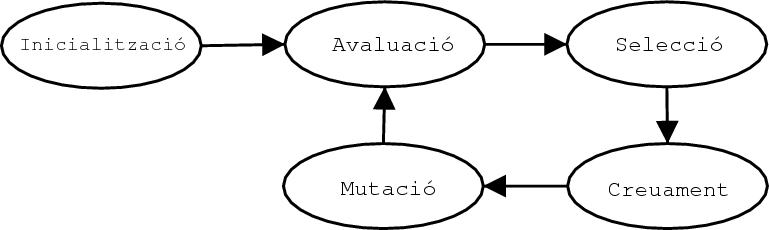
\includegraphics[width=4in]{intro/ga}
\caption{\label{fig:ga}Diagrama d'activitats d'un algorisme genètic}
\end{figure}

A grans trets, la fase d'inicialització, crea la població inicial que començarà
el procés evolutiu. Sempre cal un conjunt suficientment gran i divers per
assegurar l'èxit del procés evolutiu \cite{G02}.

Pel que fa a l'avaluació, cal dir que és un dels aspectes més importants d'un
GA, en l'apartat \ref{subsec:avaluacio} s'entrarà amb molt més detall amb aquest
afer, però cal comentar abans que la funció d'avaluació és en si mateix el
problema que es vol resoldre o optimitzar.

La selecció és el mecanisme que tria els individus que seran candidats a ser
escollits, més endavant s'entrarà en molt més detall en els mecanismes
involucrats en la selecció desenvolupada, i també es citaran altes tècniques de
selecció.

El creuament és el procés pel qual es combinen dos cromosomes que s'han
seleccionat per tenir descendència. Hi han moltes formes de fer-ho, però una de
les més habituals és un creuament discret amb un o dos punts de tall.  Aquesta
és la tècnica que hem usat en dos dels nostres projectes \texttt{Pholus} i
\texttt{Chiron}  %% refs

Finalment, vé la mutació, que és l'encarregada d'introduir o canvis aleatoris en
els individus amb una probabilitat més aviat baixa. Aquesta activitat és
realitza per estar segurs de que tot l'espai de cerca pugui ser explorat.
Modificant la probabilitat d'aparició de mutacions donem més o menys
variabilitat genètica al algorisme, afavorint o desfavorint la convergència de
la població.

En acabar la mutació el cicle es tanca, i va iterant fins que la condició
d'aturada s'assoleix. Normalment la condició d'aturada és generar un nombre
prefixat de generacions, però alguns cops també s'utilitzen criteris, com per
exemple la convergència de la població.

\subsubsection{La funció d'avaluació\label{subsec:avaluacio}} La funció
d'avaluació és vital per un algorisme genètic. Aquesta tracta de simular
l'entorn en el qual estan immerses les solucions, i ens retorna el
\emph{fitness} o el grau d'adaptació dels individus a l'entorn. Cal fer notar
que la funció d'avaluació codifica el problema que es vol que el GA resolgui.

En alguns problemes la funció d'avaluació és tan complexa que s'ha de
simplificar per aproximacions més ràpides. Fins i tot en alguns casos s'ha
observat que el fet de substituir la funció d'avaluació per una menys complexa
dóna la oportunitat d'avaluar més individus per unitat de temps, i amb aquest
increment dels individus avaluats, al final s'assoleix una solució real més
acurada que la que es va trobar utilitzant la funció d'avaluació inicial
\cite{G89}. 

\subsubsection{Reproducció} En la reproducció estan implicats dos dels tres
pilars fonamentals dels GA, la selecció i el creuament. La creació de nova
descendència és un factor crític, en la mesura que de generació en generació,
els nous individus creats van superant als seus ascendents.

A partir d'ara entra en joc el concepte de pressió selectiva. És a dir, la
pressió que d'alguna manera s'exerceix sobre la població per a que vagi
augmentant el seu grau d'adaptació a l'entorn. Sovint s'ha de vigilar amb la
pressió selectiva, per que si és massa elevada, l'algorisme no té altra
escapatòria més que arribar a solucions bones a curt termini però que no
assoleixen els màxims globals. Aquestes solucions queden estancades en màxims
locals. D'altra banda si la pressió selectiva és molt baixa, el temps de
convergència és molt llarg.  Com sempre, s'ha d'arribar a un nivell de
compromís, entre el temps de convergència i el risc de caure en màxims locals.

Cal fer notar que de vegades podria ser que alguns individus siguin seleccionats
repetits cops en una mateixa generació. Això no té per que ser dolent, ja que
normalment aquests tipus d'individus tindran un \emph{fitness} molt alt.

Quan els individus que van a ser creuats ja han estat seleccionats, sols queda
pendent emparellar en grups de dos els individus per tal de generar nova
descendència. 

Un concepte que també s'ha d'introduir és el concepte d'\texttt{elitisme}, que
implica guardar els $k$ millors individus de la població de generació en
generació, així s'assegura que els millors individus de la població no es perden
mai.  Aquest és un element que afegeix pressió evolutiva, mantenint un ``llistó''
del que no es baixa mai generació a generació, i accelerant la convergència.

\subsubsection{Convergència} 

Normalment els individus d'un GA van convergint cap als màxims de la solució de
generació en generació. Es diu que un GA ha convergit quan el 95\% de la
població té el mateix valor \cite{D75}, i una població ha convergit quan tots
els seus gens han convergit.

En alguns casos la condició d'aturada del cicle d'activitats d'un GA ve imposat
per condicions de convergència.  Quan els individus han assolit un cert nivell de
convergència (el 95\% dels individus d'una generació són iguals), en general
implica que el GA no evolucionarà més les solucions, per tant té sentit aturar
la cerca.

Quan apliquem operadors (veure secció \ref{subsec:operadors}) molt restrictius,
que donen molta pressió evolutiva, ens podem trobar en casos de
\emph{convergència prematura}, és a dir, en poques generacions, tots els
individus s'assemblen massa entre ells i els creuaments són poc efectius.  En
aquests casos, l'algorisme s'estanca en un màxim o mínim local, però rarament
global.

\subsection{Operadors\label{subsec:operadors}} 

S'entenen com els operadors d'un GA com les diferents tècniques de realitzar les
5 fases bàsiques d'un GA. En el treball final de carrera titulat com
\emph{Química combinatòria virtual: disseny de pèptids que travessen la barrera
hematoencefàlica} \cite{B01},  hi ha un ampli recull d'operadors, on s'analitzen
els punts forts i febles de cadascun.  A continuació es descriuen els operadors
emprats en el GA desenvolupat en aquest projecte en cadascuna de les fases.

\subsubsection{Inicialització} 
\label{ssub:IInicialitzacio}

Per fer les inicialitzacions es poden descriure molts mètodes, des de models
totalment aleatoris, fins a la incorporació de certes heurístiques o coneixement
sobre el problema. En aquest projecte s'ha optat per una inicialització
aleatòria, sempre i quan els cromosomes compleixin amb els requeriments del
problema.  Com s'explica en cadascun dels apartats, cada gen pot prendre un
nombre finit de valors, o com a màxim, un rang (en el cas de ser representat per
un real).

\subsubsection{Selecció}
\label{subs:Iseleccio}
La selecció és la manera en que s'escolliran els individus de la població més
ben adaptats, per a permetre que aquests siguin els ``pares'' dels individus de
la següent generació.

La selecció, en els algorismes evolutius és típicament probabilística, donant
més probabilitats de ser ``pares'' als cromosomes de més qualitat que als de
menys.  De totes maneres, els individus de poca qualitat també tenen alguna
possibilitat d'encreuar-se i així passar el seu ``codi genètic'' a generacions
futures.

Tècniques de selecció n'hi ha moltes, i aquí n'explicarem només algunes, les
que hem provat per als nostres projectes, o bé alguna d'especialment curiosa.

Els \emph{fitness proportional selection}, també anomenat selecció per ruleta
basen el seu funcionament en què per a cada selecció, la probabilitat que un
individu $f_i$ sigui seleccionat per a reproduir-se depèn únicament del seu
\emph{fitness} absolut comparat amb els fitness dels altres individus de la
població (Figura \ref{fig:rwsgraph}).

Aquest mecanisme de selecció va ser introduït a \cite{H75} i ha estat molt
estudiat en endavant.  Donada la seva simplicitat, s'han trobat diversos
problemes:

\begin{itemize}
	\item Els individus que són molt més bons que la resta, tendeixen a
	``conquerir'' la població sencera molt ràpidament. Provoca convergència
	prematura.
	\item Si els fitness dels individus són molt similars, la pressió selectiva
	es veu molt mermada, fent que a la hora d'escollir, es tingui gairebé les
	mateixes probabilitats d'escollir un individus que un altre, fent que la
	selecció segueixi una distribució uniforme aleatòria.
\end{itemize}


\begin{figure} \centering 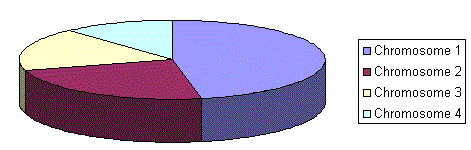
\includegraphics[width=4in]{intro/rwsgraph.png}
\caption{\label{fig:rwsgraph}Ruleta FPS}
\end{figure}

La selecció \emph{basada en ranking}, és un altre mètode que intenta
solucionar els problemes de FPS \cite{B87a}.  Aquest mètode manté la pressió
selectiva ordenant la població en funció del seu fitness, i assignant les
probabilitats de selecció en funció de la ordenació en comptes de fer-ho en
funció del propi fitness. D'aquesta manera, s'estableix una relació de qui és
millor que qui, però no hi ha els problemes que teníem en FPS.  El problema que
té aquest mètode és que no fa cap distinció entre les relacions de fitness
excepte per la relació de ser millor que un altre.  Per exemple, tres elements
amb fitness 1,2,3 s'ordenaran igual, i amb les mateixes probabilitats de ser
seleccionats que elements amb fitness 1,100 i 1000 .  La manera que es té de
mitigar (que no solucionar) aquest problema és assignar proporcions escalades en
relació entre la posició en el ranking i la probabilitat de ser seleccionat,
pot ser una relació lineal, exponencial o bé logarítmica. 

En la figura \ref{fig:rank1} es mostra  un cas on hi ha un cromosoma que tindria
el 90\% de probabilitats de ser escollit. El que es fa és ordenar de pitjor a
millor, i al pitjor donar-li un ``calaix'', al següent dos, al següent tres, i
finalment, al millor quatre. 

\begin{figure} \centering 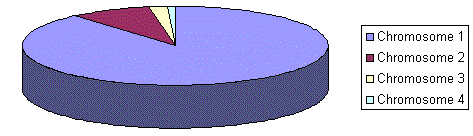
\includegraphics[width=4in]{intro/rank1.png}
\caption{\label{fig:rank1}selecció ranking}
\end{figure}

En casos reals, s'utilitzen sistemes una mica més sofisticats, com per exemple
la \emph{selecció per torneig}.  En una selecció per torneig s'ha de definir
un paràmetre $N$ que descriu la mida del torneig.

En la selecció per torneig, per decidir quin individu passarà a la següent
generació, es realitzen ``enfrontaments'' de $N$ individus, comparant el seu
fitness.  El que guanya de tots ells serà qui passarà a la fase de creuament.

Una de les avantatges que té aquest mètode és que no fa falta tenir
comptabilitzats tots els fitness de la població sencera, ja que només s'han
d'avaluar per grups de $N$.  Això el fa molt còmode d'usar en sistemes
paral·lelitzats, o bé en problemes on es molt costós fer una ordenació dels
fitness a nivell global, com per exemple, quan avaluem tirades en un joc
estratègic.

Hi ha variants de tornejos on, es defineix un altre paràmetre, que és la
probabilitat que el que té millor fitness surti realment guanyador.  En els
tornejos normals (deterministes), aquest paràmetre $p=1$, però si el disminuïm
tal que $p<1$, hi haurà un numero de casos $1-p$ on no guanyarà el millor.
Aquesta tècnica redueix la pressió evolutiva permetent que individus pitjors,
passin el seu codi genètic a següents generacions, augmentant la diversitat.

L'algorisme esquematitzat (tant per p=1 com per p<1) és el següent:

\begin{itemize}
	\item S'escullen $N$ individus de la població aleatòriament.
	\item S'agafa el millor individu amb probabilitat $p$.
	\item S'agafa el segon millor individu amb probabilitat $p \times (1-p)$
	\item S'agafa el tercer millor individu amb probabilitat $p \times (1-p)^2$
	\item \ldots
\end{itemize}


%En aquest projecte s'ha utilitzat una selecció \emph{stochastic
%universal samplig} \cite{B87a} amb \emph{rank selection} \cite{B87b} i una
%tècnica d'especiació coneguda com \emph{sharing} \cite{33}.

\subsubsection{Creuament}

Un cop s'han seleccionat els individus de la nova població, aquests podran tenir
descendència. Per a cadascun d'ells es genera un nombre aleatori entre 0 i 1, i
si no supera una determinada probabilitat de creuament, normalment bastant alta,
és copiat directament a la següent fase que és la mutació.

Els individus escollits per creuar-se són agrupats en parelles aleatòries, i
s'aplica un creuament clàssic discret unipunt.  Es genera un punt de tall del
cromosoma de forma aleatòria, i es construeixen dos descendents. El primer
descendent contindrà la primera part del material genètic del primer progenitor
fins el punt de tall, i la segona part del segon progenitor, que va des del punt
de tall fins el final del cromosoma. El segon descendent serà a l'inrevés, la
primera part serà directament la primera part del segon progenitor, i la segona
part la segona del primer progenitor.

En els dos problemes de GA hem utilitzat el creuament unipunt, però també hi
ha variants d'aquest creuament utilitzant dos o més punts.  Com es veurà en les
seccions de cadascun dels problemes, s'han fet proves amb aquests creuaments,
però no ens han donat resultats millors, i hem seguit amb els creuaments
unipunt.

Aquests creuaments, es poden aplicar amb seguretat quan considerem que la
relació d'un gen $i$ amb el gen $i+1$ no és forta (no hi ha epistàcia).  Si
trencant un cromosoma per la posició $i$, destruïm algun \emph{building block},
probablement, es perdrà un factor que feia que l'individu fós bo, i al
creuar-lo, no obtindrem gaire bons resultats.

\subsubsection{Mutació}

Finalment, abans de tancar el cicle, es realitza la mutació. Aquesta activitat
aplica mutacions de forma aleatòria, però amb una baixa probabilitat, als gens
dels individus de la nova generació que està a punt de crear-se. En el cas de
disposar d'elitisme, aquests individus no són exposats a les mutacions.

L'operador de mutació emprat és clàssic uniforme. Això implica que els gens
seleccionats per a ser mutats, se'ls canvia el seu valor de forma aleatòria
però, el nou valor pertany al domini de la variable de decisió que codifica
aquell gen.

\subsubsection{Reemplaçament}

El model de reemplaçament seleccionat és el conegut com elitisme, que com ja
s'ha explicat abans, crear tota una nova població d'individus de generació en
generació. Malgrat això els $k$ millors individus van guardant-se per tal
d'assegurar que no es perden al llarg del procés evolutiu.  En tots els
projectes que es presenten en aquest treball, s'ha mantingut la mida de la
població, però també es possible fer que aquesta mida de la població varii al
llarg de les generacions.

%\subsection{Teoremes} En general no n'hi ha cap teoria universalment acceptada
%del perquè funcionen bé els GA, ni del perquè de la seua robustesa. Però n'hi
%han dues hipòtesis que són interessants conèixer per que ens poden ajudar a
%implementar bones aplicacions dels GA, i cada cop més estan adoptant-se pels
%teòrics com els vertader mecanismes que fan evolucionar els GA. El primer
%d'ells és el teorema de la disposició, i el segon la hipòtesi dels blocs de
%construcció, o \emph{building blocks}.

%\subsubsection{Teorema de la disposició} Més conegut per \emph{schema theorem},
%va ser proposat per Holland \cite{H75}. Un \emph{schemata} és un patró de
%valors dels gens en binari. On aquest patró està format \{1, 0, \( \star  \)\}
%sent \( \star  \) el caràcter comodí. De tal forma que cromosomes com
%{}``0000'', {}``0010'', {}``0001'' i {}``0011'' corresponen al mateix patró
%{}``00\( \star \star  \)''.

%Aquest teorema diu que els individus bons, ho són per que tenen un bon patró.
%Llavors hem de donar-los a aquests individus més possibilitats de reproducció
%en funció del seu \emph{fitness}.  Per tant al passar aquests patrons a la
%descendència i al aplicar-los aquest mateixa filosofia, anem augmentant les
%possibilitats de generar millors patrons a mesura que passa el temps.

%Segons Holland si distribuïm aquestes probabilitats en funció de la proporció
%del \emph{fitness} d'un individu a seleccionar front al de la resta, un bon
%patrons estarà tenint un nombre de possibilitats que va creixent
%exponencialment. També va dir que el nombre de patrons que estant sent
%processats en una generació, és n\( ^{3} \), on n és el tamany de la població.
%Això és conegut com paral·lelisme implícit.

%\subsubsection{Hipòtesi sobre els blocs de construcció \label{subsec:bb}}
%Goldberg, en canvi, formula la \emph{Building Block Hypotesis} \cite{G89}.  Que
%diu que la potència dels GA's recau sobre l'habilitat de crear bons blocs de
%construcció. Aquests són curts patrons amb una longitud fixa, que funcionen
%molt bé per separat; independentment de la resta del cromosoma. I que si se li
%és incorporat un bon bloc de construcció a un cert individu, el seu
%\emph{fitness} augmenta. 

%Per afavorir la aparició de blocs de construcció, la codificació del cromosoma
%hauria de tenir propers els gens relacionats, i al mateix temps, que la
%interacció entre els gens siga mínima.

%La no interacció entre gens vol dir que l'aportació d'un gen al còmput del
%\emph{fitness} no es vegi afectat per els valors que poden prendre altres gens.
%Més tard Goldberg va publicar els estudis teòrics sobre gens que sí que
%interaccionen entre ells i com aprendre aquestes interaccions
%\cite{Goldberg:2002}, això és conegut com \emph{linkage learning}, i amb
%l'algorisme BOA que en la secció \ref{EDA} s'explicarà, es poden arribar a
%salvara aquest tipus d'inconveniències. Cal dir que en aquest projecte el
%còmput del \emph{fitness} si que s'espera que es veja afectat per la
%interrelació entre gens.

\section{Programació d'expressions genètiques} % (fold)
\label{sec:Programacio d'expressions genetiques}

La programació d'expressions genètiques (GEP), podríem dir que és una evolució de
la programació genètica (GP) en tant que intenta solucionar el mateix tipus de
problema.  A diferència dels GA clàssics, que tracten de solucionar (al menys de
forma natural) problemes d'optimització, tant GP com GEP podríen ser
classificats dins dels algorismes d'aprenentatge.  Per posar un exemple, en la
majoria de GA, el que es busca optimitzar és una entrada per a un procés
(Figura \ref{fig:ch1-4}).  En canvi, en GEP i GP el que es busca és un procés que
optimitzi una entrada donada (Figura \ref{fig:ch1-5}).

\begin{figure} \centering 
\includegraphics[width=4in]{intro/1-4.jpg}
\caption{\label{fig:ch1-4}Optimització d'entrada}
\end{figure}
\begin{figure} \centering 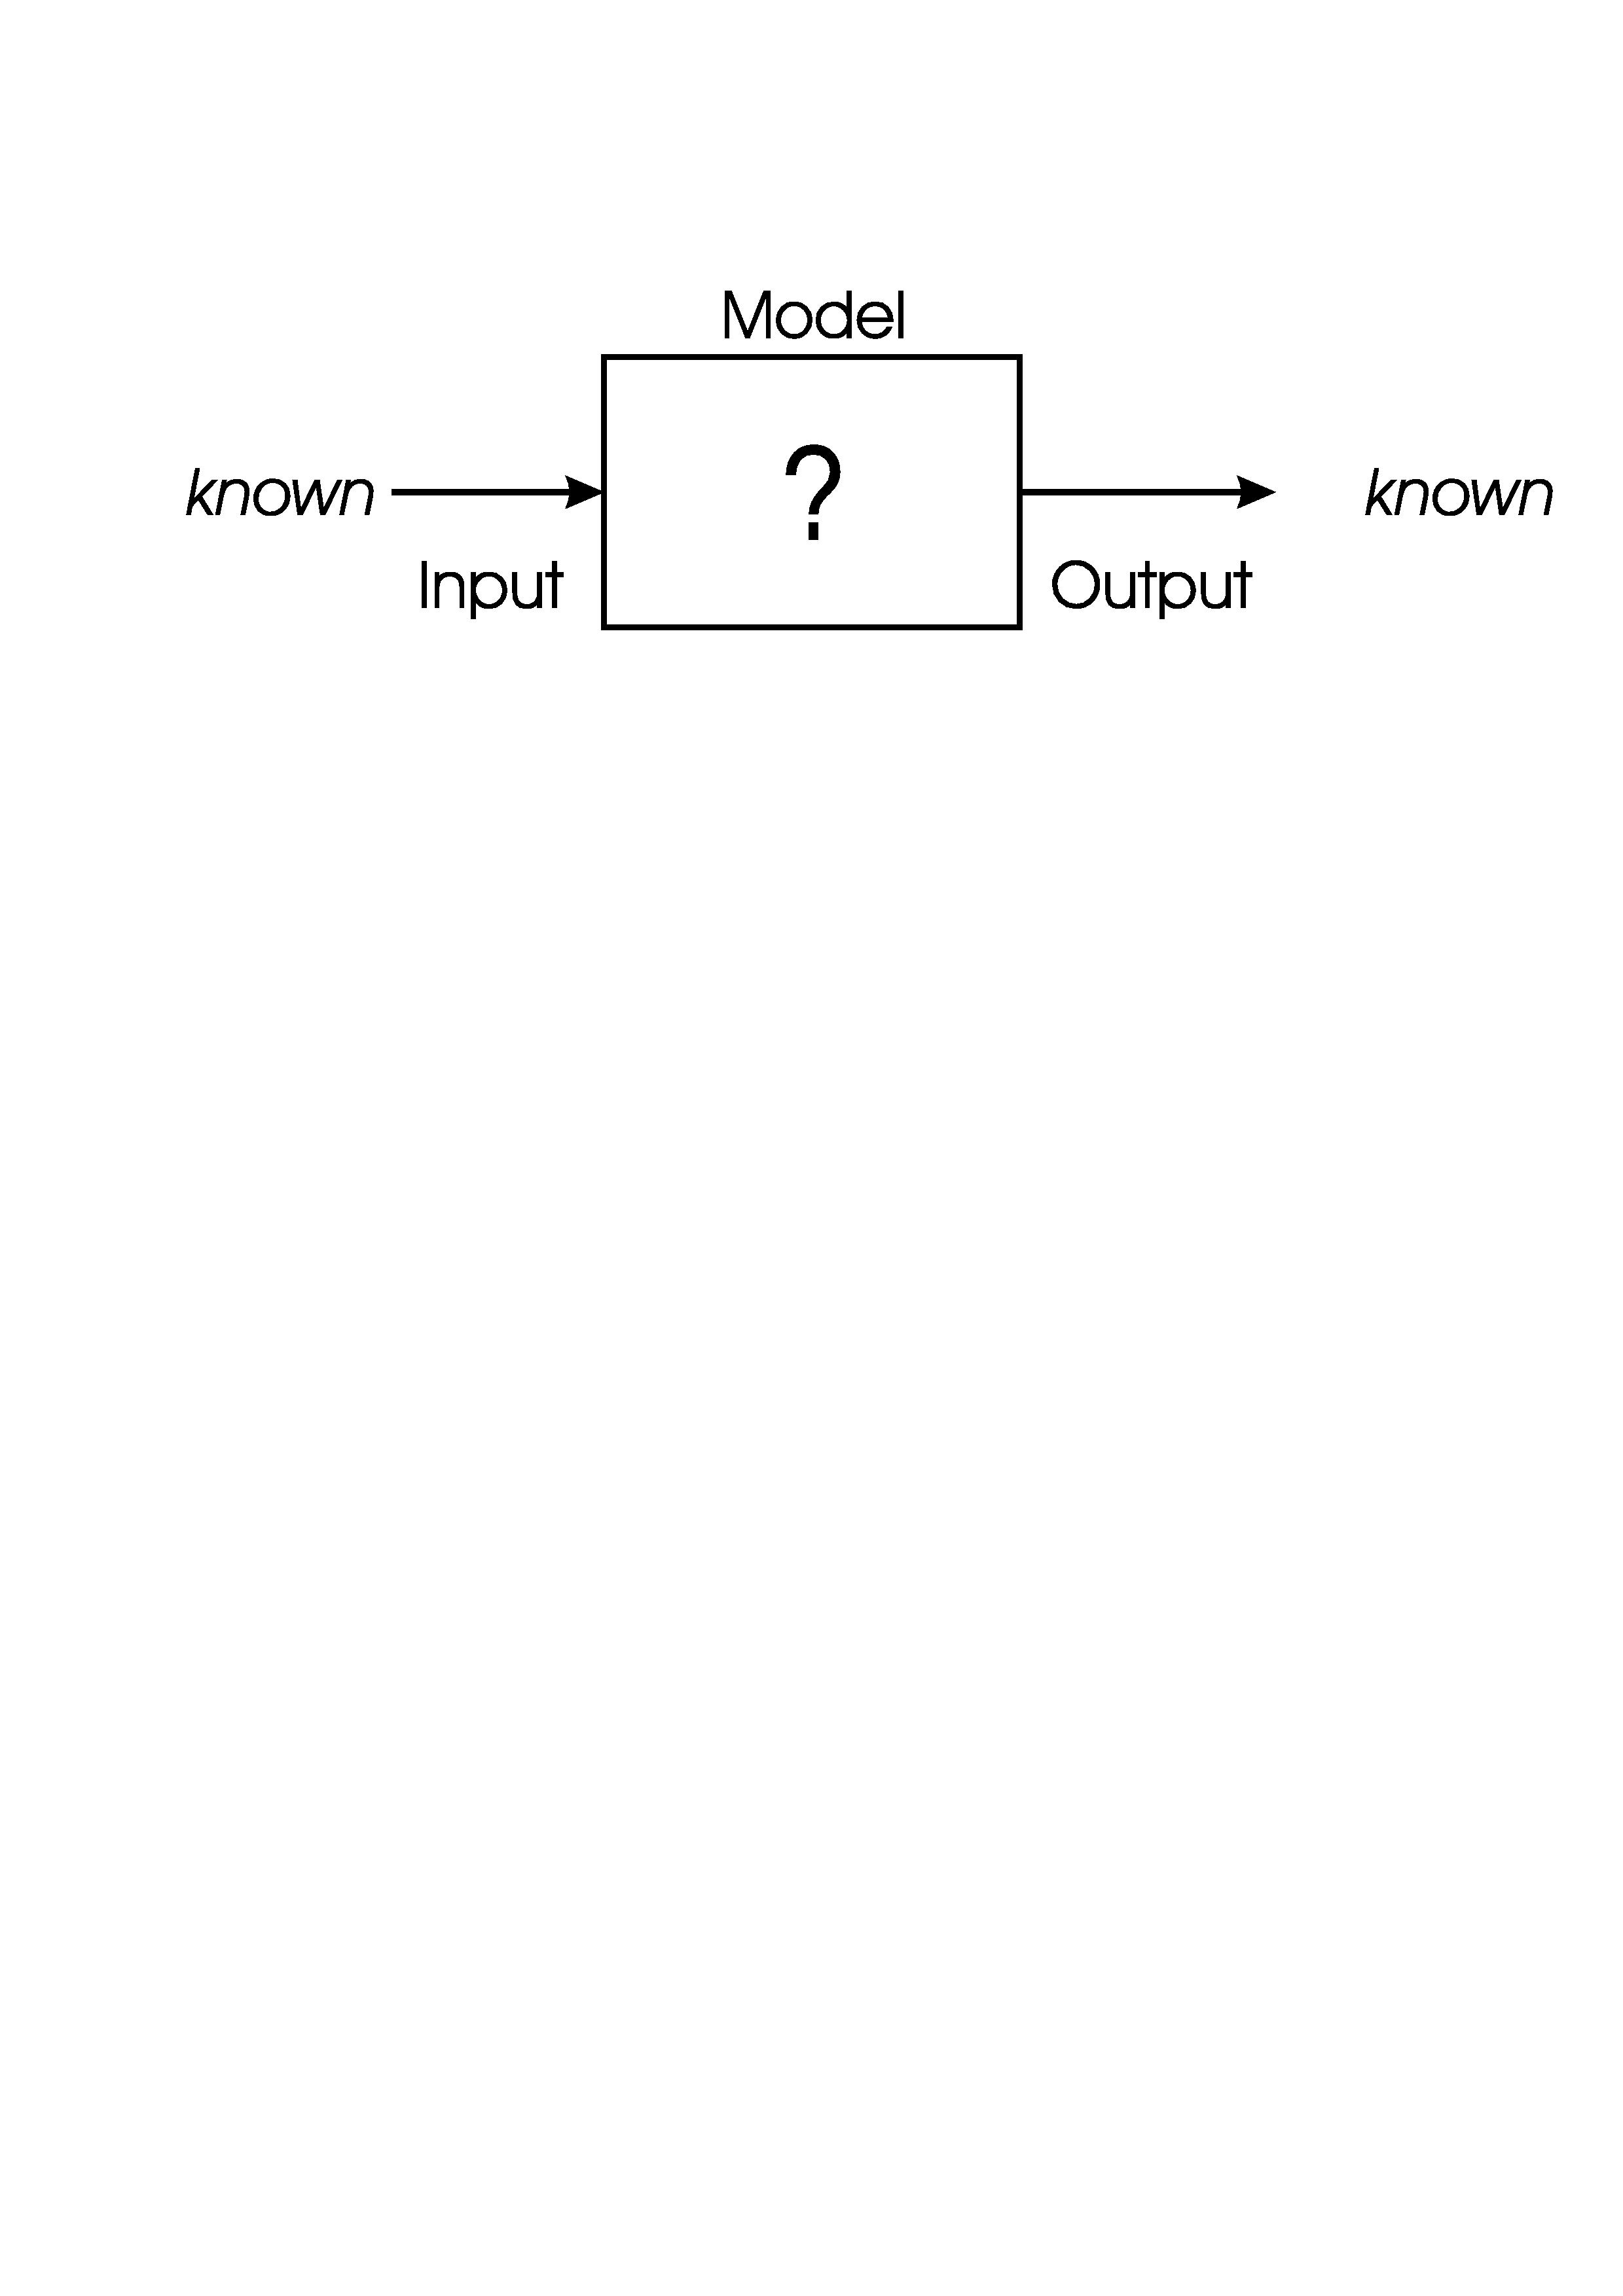
\includegraphics[width=4in]{intro/1-5.jpg}
\caption{\label{fig:ch1-5}Optimització procés}
\end{figure}

Els processos que s'intenten optimitzar, contenen, és clar, molta més informació
que en un dels algorismes genètics dels que s'han vist fins ara.  Això és
evident, ja que aquí, els individus són parts funcionals d'un sistema i no
només dades que un sistema agafarà i avaluarà.  Tot seguit es mostren tres
exemples de possibles problemes que es poden optimitzar:

\begin{itemize}
	\item Fórmules lògiques (per exemple $ (x\land true) \rightarrow ((x \lor y)
		\lor (z \leftrightarrow ( x \land y)))$ ). Figura \ref{fig:6-2-2}.
	\item Fórmules aritmètiques (per exemple $2\times\pi+((x+3)-\frac{y}{5+1})$
		).  Figura \ref{fig:6-2-1}
	\item Programes 
		\begin{verbatim}
				i = 1;
				while (i<20){
					i = i + 1;
					}
		\end{verbatim}. Figura \ref{fig:6-3}.
\end{itemize}

\begin{figure} \centering 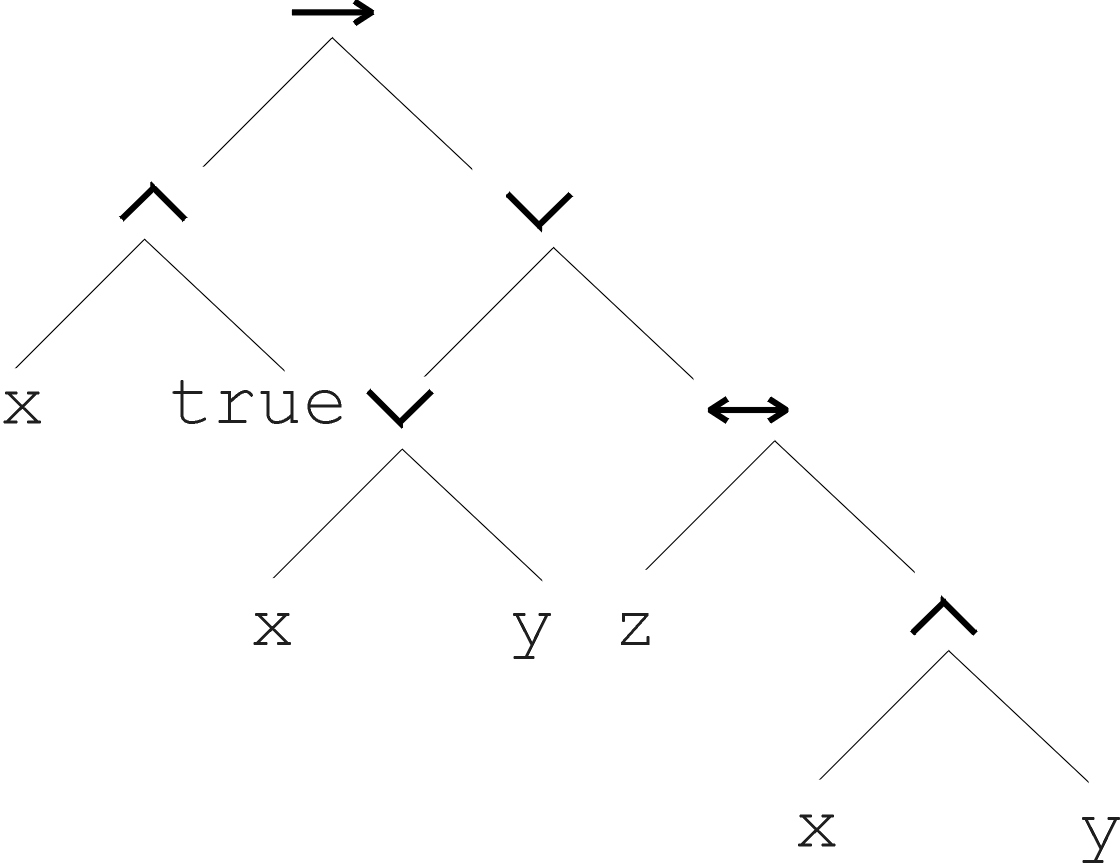
\includegraphics[width=4in]{intro/6-2-2.jpg}
\caption{\label{fig:6-2-2}Fórmula logica}
\end{figure}

\begin{figure} \centering 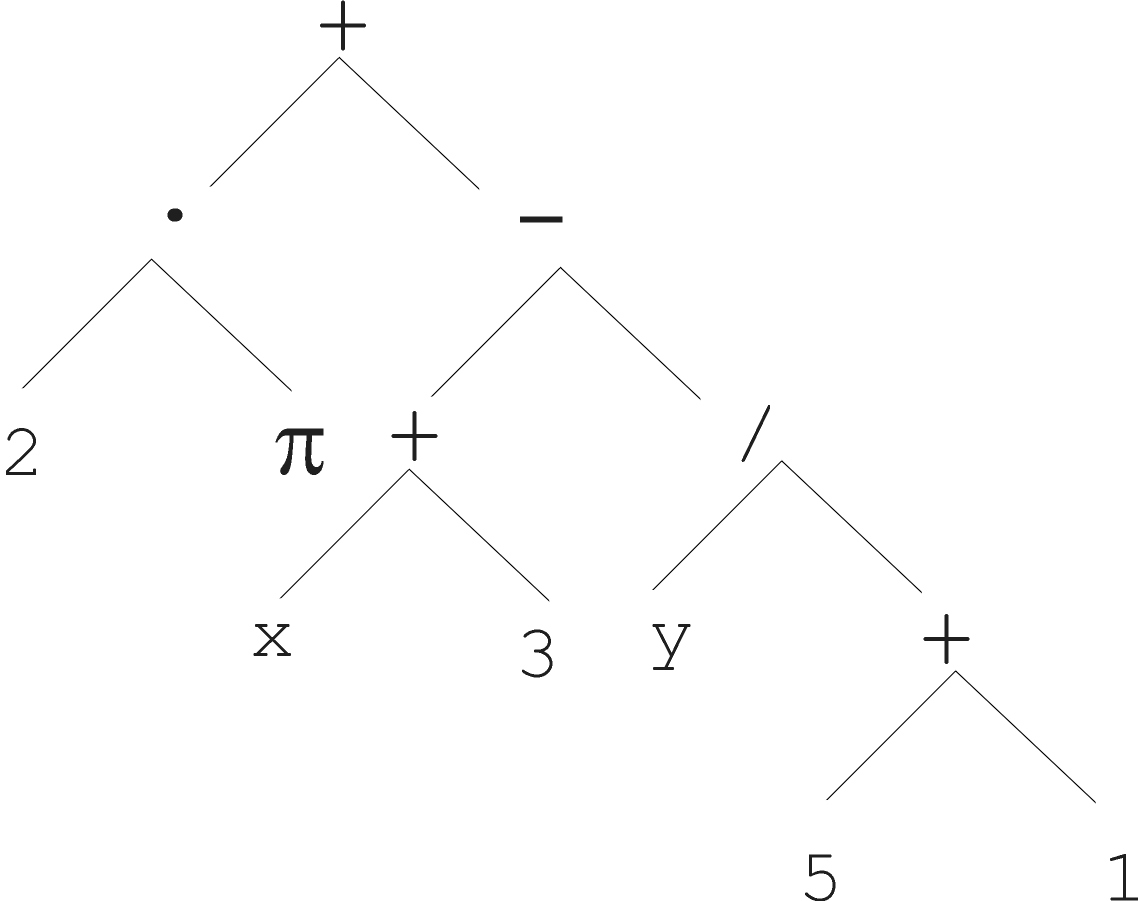
\includegraphics[width=4in]{intro/6-2-1.jpg}
\caption{\label{fig:6-2-1}Fórmula aritmètica}
\end{figure}

\begin{figure} \centering 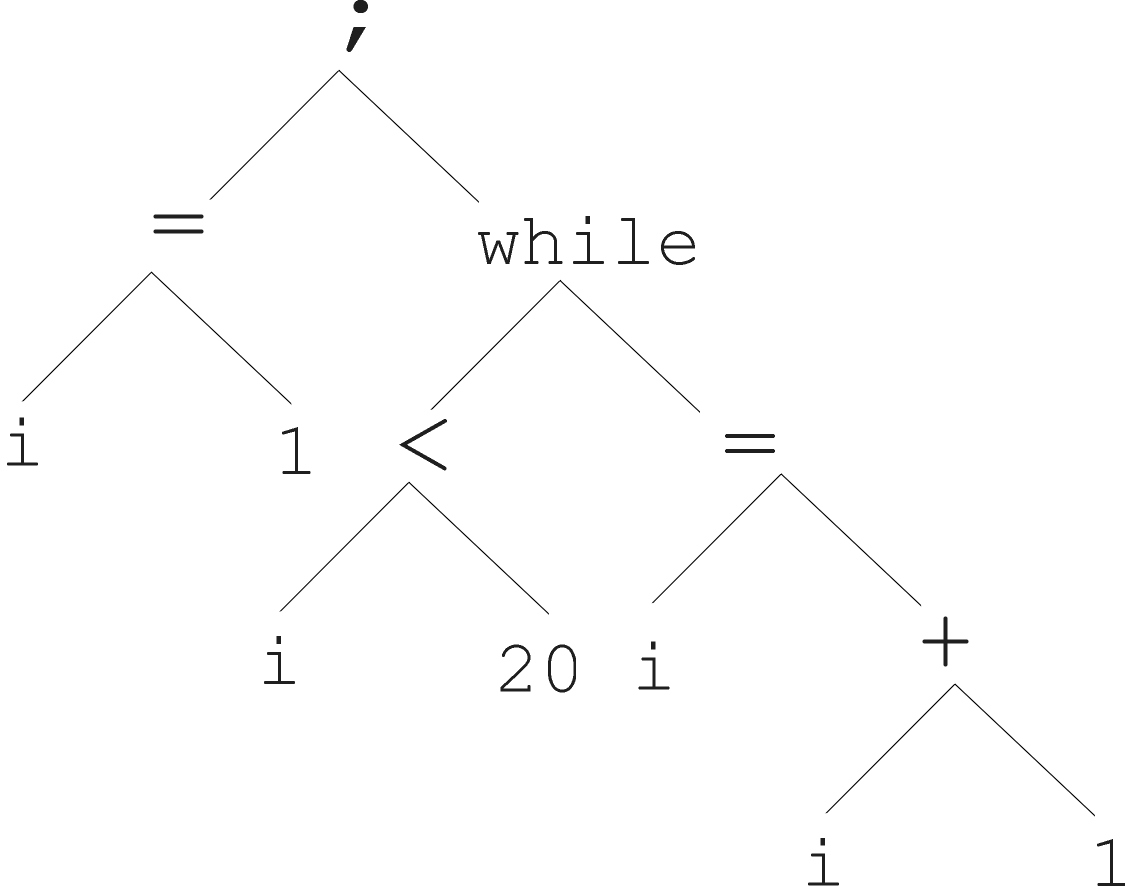
\includegraphics[width=4in]{intro/6-3.jpg}
\caption{\label{fig:6-3}programa}
\end{figure}

En aquest tipus d'algorismes, els individus no poden ser codificats com a un
sol vector de bits o reals, i aquests ser tractats independentment uns dels
altres, sinó que el que han de codificar els individus són arbres.  Per tant,
la seva codificació és més complexa, havent-hi una clara separació entre genotip
i fenotip.

Estrictament parlant, però, no hi ha cap altra diferència entre els GA clàssics
i GP o GEP.  Simplement, aquí interpretem els cromosomes com a arbres.

A continuació es farà una breu introducció a GP, per saber els orígens de
GEP, i seguirà una explicació una mica més detallada de GEP, que és la tècnica
que s'ha utilitzat en \texttt{GEP}.

\subsection{Antecessors: Programació Genètica} % (fold)
\label{sub:Ant. Programacio Genetica}
La programació genètica és una de les diferents disciplines dins dels algorismes
evolutius, inventat per Cramer en el 1985 (\cite{C85}) i després millorat per
Goldberg (\cite{Goldberg:89}) i
John Koza en 1992 (\cite{koza:92}) basat en la solució de problemes amb genotips de
llargada fixa, però interpretats de forma no lineal (arbres) de mida i formes.

Els individus en GP, normalment tenen un alfabet més ric que els algorismes
evolutius clàssics, però aquesta riquesa que ofereix tractar els cromosomes amb
una interpretació no lineal, fa que aquests individus no siguin autònoms, i no
poden funcionar com a genotip i fenotip alhora, ja que han de passar per una
fase de ``traducció''.

Per poder diferenciar la programació genètica de la programació d'expressions
genètiques, fem un repàs molt ràpid dels operadors més comuns en GP.

\subsubsection{Operadors} % (fold)
\label{ssub:operadors}

Els algorismes de programació genètica tenen els mateixos operadors que els
altres AE, però amb la diferència notable que s'ha de tenir en compte que al fer
una modificació sobre el genotip, el fenotip pot veure's modificat de manera
``no prevista'' si no anem molt en compte.  Per exemple, al fer un creuament
entre dos individus, el cromosoma resultant, pot no mantenir cap (o gairebé
cap) característica dels seus pares, donada la no-linealitat dels fenotips
respecte els genotips.  Això dona lloc a que molts dels individus generats a
partir de individus vàlids, són invàlids en el sentit que poden no complir les
condicions bàsiques per a ser traduïts a fenotips i posteriorment avaluats.

Una manera de assegurar que les propietats dels progenitors es mantenen a la
descendència i que continuen essent individus vàlids, és aplicar els operadors
a nivell de fenotip, i assegurant-se que els fills continuen tenint una mínima
entitat que els fa avaluables en el context del problema.  Això dificulta molt,
però, la programació dels operadors.

Per exemple, en el cas d'interpretar els genotips com a arbres amb formules
matemàtiques, al fer creuaments podem fer-los per subarbres, agafant l'arrel i
el fill esquerra del arbre d'un dels dos progenitors, i el fill dret de l'altre.
Tot seguit es comenten els dos operadors més interessants en programació
genètica.

\paragraph{Mutacions} % (fold)
\label{par:Mutacions}
Les mutacions en programació genètica són similars conceptualment a les que
trobem en els altres algorismes evolutius, canviant un subarbre aleatori del
cromosoma per un altre subarbre generat aleatòriament.  Veiem aquí la diferència
necessària en la implementació, ja que la mutació té lloc en l'espai del fenotip
(arbre) i no pas en el genotip (vector de símbols).  Hi ha hagut controvèrsia
sobre la aplicació de mutacions en programació genètica des de els seus inicis.
Koza en \cite{koza:92} aconsellava desactivar per complet la mutació.   Més
endavant, s'ha anat donant una mica més importància, però sense ser mai un
operador fonamental, donat que el creuament també actua en certa manera
d'operador de mutació però a més gran escala.  Aquestes mutacions canvien la
mida dels cromosomes.
% paragraph Mutacions (end)

\paragraph{Creuament} % (fold)
\label{par:Creuament}
El creuament de cromosomes en programació genètica és un operador binari que
consisteix en intercanviar dos subarbres entre dos cromosomes d'una població.
Una altra vegada, perquè el creuament no doni lloc a elements sintàcticament
incorrectes, el creuament s'ha de realitzar a nivell d'arbre, provocant també
canvis en la mida dels cromosomes.

% paragraph Creuament (end)

% subsubsection operadors (end)
% subsection Ant. Programació Genètica (end)

\subsection{Principis bàsics} % (fold)
\label{sub:Principis Basics}

La programació genètica, però, té alguns problemes fonamentals, que mermen la 
seva potència, com són el sobreentrenament (és molt fàcil obtenir 
solucions sobreentrenades per al conjunt de mostres amb el que entrenem
 l'algorisme), el \emph{bloat} (els arbres, tendeixen a créixer desmesuradament),
o bé la mateixa complexitat que té fer els creuaments o mutacions a nivell de 
fenotip. GEP, intenta solucionar alguns d'aquests problemes.


En GEP, els principals elements son els cromosomes i els arbres d'expressions,
on els segons són la expressió del la informació genètica codificada en els
cromosomes.  Com en la natura, el procés de descodificació s'anomena
\emph{traducció}.

La correspondència d'un a l'altre ha de ser unívoca i hi ha unes regles que ens
permeten passar d'un a l'altra.  En la natura, aquesta traducció no és pas tant
fàcil, ja que no se sap gairebé res del genotip, si tenim només un fenotip, però
per a tenir una traducció fàcil dins de GEP, es disposa d'una notació anomenada
\emph{Karva Notation} que ens permet fer les traduccions en les dues direccions
fàcilment \ref{ssub:Notacio Karva}.

% explicar constants


%http://www.gene-expression-programming.com/Tutorial002.asp
\subsubsection{Notació Karva} % (fold)
\label{ssub:Notacio Karva}

La notació Karva, és una manera de representar qualsevol expressió matemàtica o
lògica en una estructura lineal de manera que es pugui traslladar a un arbre
fàcilment \cite{ferreira:2001} i \cite{ferreira:2006}.

Les estructures lineals que conformen els individus en GEP són els cromosomes,
i cada cromosoma té un o més gens, que aquí prenen un altre significat més
ampli, no referint-se als ``àtoms'' indivisibles (com en els AE que hem vist
fins ara) sinó que cada gen està associat a una K-expression.
\cite{ferreira:2007}

Tot seguit es mostra un exemple d'un gen, i en \ref{fig:expression tree1} el seu
\texttt{Arbre d'expressió} equivalent

\begin{verbatim}
0123456    
+/*abcd
\end{verbatim}

\begin{figure}[h]
\begin{center}
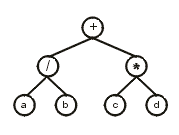
\includegraphics{intro/et1.png}
\end{center}
\caption{Arbre d'expressió}
\label{fig:expression tree1}
\end{figure}

La traducció d'un a l'altre és directe.  El primer element en el gen (posició
0) correspon a la arrel del arbre.  Llavors, sota d'aquest node, s'enganxen
tants nodes fills com arguments tingui la funció representada pel node arrel
(dos en aquest cas). Els nodes fills es van omplint recursivament, consumint
símbols del cromosoma, fins que un nivell del arbre queda només omplert per
nodes terminals, que no son més que nodes on el símbol que contenen té aritat
zero.

Més formalment, tant el gen com l'arbre \ref{fig:expression tree1} poden ser
representats per la expressió matemàtica:

	$\frac{a}{b}+c \times d$

Per assegurar que els arbres que es creïn siguin sintàcticament vàlids, es
divideix un gen en dues parts, amb mides que segueixen unes normes determinades
que s'expliquen en detall en l'apartat \ref{ssub:Inicialitzacio}.  Un gen es
composa de la primera part (\emph{head}) que conté funcions i terminals, i d'una
segona part (\emph{tail}) que només conté terminals (aritat zero). Si el tail és
suficientment llarg com per omplir la última capa del arbre que genera el propi
gen, sempre hi haurà prou operands per a donar a les funcions.

% subsubsection Notació Karva (end)

\subsubsection{Individus} % (fold)
\label{issub:individus}
% subsubsection individus (end)

Com s'ha explicat en \ref{ssub:Notacio Karva}, els individus son representats en
una tira de símbols (genotip), però al interpretar-los i avaluar-los, tenen una
representació en forma d'arbre d'expressió similar a un AST\footnote{Abstract
syntax tree}.

Un individu o cromosoma està format per un o més gens.  En la versió més
primària, un cromosoma conté només un gen, però es poden combinar diversos gens,
creant cromosomes multigen, com s'explicarà més endavant.

En aquest tipus de notació, existeixen el que denominem ``zones
no-codificadores'', que són parts del gen, que per diversos motius formen part
del genotip, però no tenen representació, ni es mostren en el fenotip.  Un
exemple d'això és


\begin{verbatim}
	01234567890123456 	 
	Q/a*+b-cbabaccbac
\end{verbatim}

On la $Q$ representa l'arrel quadrada.  En aquest gen, té el i \emph{head} (que ocupa
de la posició 0 a la 7) de llargada, i el tail (de la 8 a la 16) de llargada 9.
El head té tan funcions com terminals, i el tail, només té terminals.

La codificació d'aquest gen es mostra en \ref{fig:unfinished} mostra com en aquest cas,
no han fet falta tots els elements del gen per a construir l'arbre.  Això és
perquè la fórmula que en assegura tenir prou tail, preveu el pitjor dels casos,
essent tots els elements del head funcions amb la màxima aritat.  Com que en
aquest cas, tenim una arrel quadrada (i en l'arrel del arbre), deixem de
necessitar gairebé la meitat del gen per a fer la traducció.

\begin{figure}[h]
\begin{center}
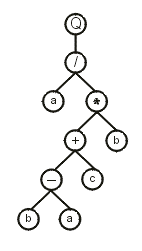
\includegraphics{geptut/pt02.png}
\end{center}
\caption{Arbre d'expressió}
\label{fig:unfinished}
\end{figure}

Aquests trossos de cromosoma que no s'utilitzen, participen igualment en els
creuaments (es fan a nivell de vector de símbols), i fan que una mutació en una
zona del \emph{head} ``activi'' una zona prèviament inactiva.  Això dona tant
als creuaments com a les mutacions molta més versatilitat que en els algorismes
clàssics.

Aquesta elegància de la programació d'expressions genètiques és la clau del
funcionament de GEP.  La codificació Karva és el nucli del bon funcionament de
GEP, però és només el principi.  És a dir, existeixen mètodes més avançats que
parteixen d'aquesta base, i aconsegueixen millorar els resultats del GEP
estàndard, com per exemple, codificar més d'un gen en un cromosoma. Són els
anomenats cromosomes multigen.  En aquests sistemes, els cromosomes estan
codificats a partir de diversos gens, i cadascun d'ells formen un subarbre o
subprograma.  Una vegada traduïts cadascun dels subarbres, aquests poden ser
connectats entre ells de diferents maneres.  Una de les més utilitzades és usant
funcions especials, anomenades d'enllaç. Aquestes funcions uneixen linealment
els diferents subarbres per ordre d'aparició en el gen.  Per exemple, observem
el següent cromosoma, composat per tres sub-gens.
	%XXX

	\begin{center}
	\begin{verbatim}
	012345678012345678012345678 	 
	*aQ+abbaa/Q*/aababa*+Qaabba
	\end{verbatim}
	\end{center}


Aquest cromosoma codifica tres arbres de la Figura \ref{fig:tres sub-et}

\begin{figure}[h!]
\begin{center}
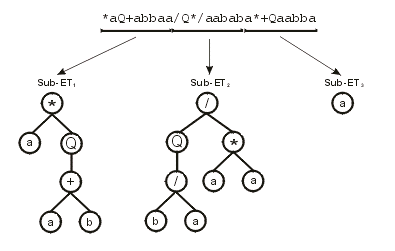
\includegraphics{geptut/pt03a.png}
\end{center}
\caption{Cromosoma representant tres sub-arbres}
\label{fig:tres sub-et}
\end{figure}

Si s'utilitzen funcions d'enllaç, per exemple, la suma, la avaluació del
cromosoma complet passaria a ser el mostrat en la figura 
\ref{fig:tres sub-et amb link}

\begin{figure}[h!]
\begin{center}
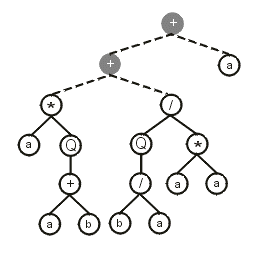
\includegraphics{geptut/pt03b.png}
\end{center}
\caption{Representació dels tres sub-arbres enllaçats amb la operació suma}
\label{fig:tres sub-et amb link}
\end{figure}

La implementació del individu que hem programat ha estat una versió una mica més
avançada que la de les funcions d'enllaç, que utilitza un dels subarbres, com a
metadada, on els terminals no es refereixen a terminals de la funció, sinó que
són referències als altres subarbres, que sí tenen com a fulles les entrades de
la funció objectiu.

%XXX
%\subsubsection{Esquema Bàsic} % (fold)
%\label{ssub:Esquema Basic}
%% subsubsection Esquema Bàsic (end)

%\subsubsection{Funció d'avaluació} % (fold)
%\label{ssub:funcio d'avaluacio}
%% subsubsection funció d'evaluació (end)
%% subsection Principis Bàsics (end)

\subsection{Operadors} % (fold)
\label{sub:Operadors}

Tot seguit es descriuran els operadors usats en GEP, sense concretar la seva
implementació, sinó explicant com varien els individus.  Per a veure els
detalls sobre la aplicació en aquest projecte, les explicacions i
implementacions més complertes consultar la secció \ref{cha:GEP}.

\subsubsection{Inicialització} % (fold)
\label{ssub:Inicialitzacio}
Donades les particularitats de la notació Karva, la inicialització d'arbres
aleatoris, consisteix en omplir head i tail amb símbols aleatoris permesos en
cadascuna de les zones.  Normalment, el head tindrà símbols operadors i
variables terminals i el tail, únicament contindrà variables terminals.  La
aritat zero dels terminals ens garantitza que l'arbre serà sintàcticament
correcte.

La població inicial es genera aplicant aquest algorisme a cadascun dels
individus.
% subsubsection Inicialització (end)

\subsubsection{Selecció} % (fold)
\label{ssub:Seleccio}
En GEP, també s'utilitza, per norma general la selecció per ruleta
(secció \ref{subs:Iseleccio}).  Un individu té una probabilitat de ser seleccionat per a
la reproducció proporcional al seu fitness en valor absolut, respecte als altres
individus de la població.

% subsubsection Selecció (end)

\subsubsection{Creuament} % (fold)
\label{ssub:Creuament}

El creuament, juntament amb la mutació és l'element que dóna la major part de la
riquesa als algorismes GEP.  Els creuaments en GEP són uns operadors que, a
diferència de la programació genètica, donen molta llibertat per a la
experimentació, ja que només s'han de mantenir unes certes regles molt bàsiques,
i es pot assegurar que es generaran arbres sintàcticament correctes.

Per exemple, en GEP es poden aplicar creuaments típics dels algorismes evolutius
clàssics, com el \texttt{creuament per un punt}, o els \texttt{creuaments per
diversos punts}, ja que si no variem la mida de la descendència, sempre es
mantindran certes les regles de què el tail no contingui mai operands (nodes
d'aritat $>0$).

A més a més, GEP té uns creuaments particulars, anomenats \texttt{recombinació
de gens}, que es basen en separar els dos individus a creuar en els seus
diferents gens, i fer el creuament ajustant els punts de tall als límits dels
gens.  Aquest creuament només és aplicable si implementem individus multigen.
% subsubsection Creuament (end)

\subsubsection{Mutació} % (fold)
\label{ssub:Mutacio}
Les mutacions, igual que els creuaments, també es poden dividir en dos
subconjunts, els que són totalment portables del món dels AE clàssics, i els
particulars de GEP.

Una mutació dels AE clàssics pot ser, per exemple, l'alteració d'un símbol
aleatori.  L'únic que s'ha de tenir en compte, és quina posició del gen s'està
mutant, per a no incloure en el tail símbols que estan restringits a usar-los
només en el head.

Per altra banda, GEP disposa de tres mutacions pròpies, anomenades IS, RIS i
``translació de gen'', que es basen en desplaçaments de conjunts de símbols al
llarg del gen.  Aquests operadors estan explicats més en detall a \ref{par:IS},
\ref{par:RIS} i \ref{par:Translacio de gen}
% subsubsection Mutació (end)

\subsubsection{Reemplaçament} % (fold)
\label{ssub:Reemplacament}

Pel reemplaçament tmabé s'utilitza elitisme, on mantenim el millor dels
individus per a la següent generació.  Les poblacions no cambien de 
mida.

% subsubsection Reemplaçament (end)
% subsection Operadors (end)
% section Programació d'expressions genètiques (end)

\section{Estat de l'art} % (fold)
\label{sec:Estat de l'art}

Actualment, els algorismes genètics estan essent més i més utilitzats no sols en
el món acadèmic, sinó també en el món de l'empresa. 


Les últimes publicacions referents a algorismes genètics tendeixen cap a
optimitzacions de la convergència.  Els algorismes genètics són processos
estocàstics (la durada o nombre d'iteracions fins a aturar-se no és un valor
conegut a priori).  Així doncs, el que s'intenta és aconseguir ``guiar''
l'algorisme perquè avanci de pressa cap a un estat convergent (s'aturi), sense
perjudicar això a la eficàcia.  Molts dels estudis de tècniques per millorar
l'eficiència dels algorismes genètics estan relacionats amb l'aprofitament de la
paralelització de processos, aprofitant sistemes distribuïts, o fins i tot en
cloud.  

Els treballs més recents relacionats amb algoritmes evolutius estan relacionats
amb la utilització de entorns de treball (frameworks) i paradigmes de
programació paralela, com poden ser hadoop o MapReduce \cite{VLCG09}.

\subsection{Tecnologia} % (fold)
\label{sub:Tecnologia}

Des dels inicis de la programació, el llenguatge per excelència
relacionat amb la intel·ligència artificial ha estat lisp \cite{JMC59}, creat per John
McCarthy el 1958 donat la gran flexibilitat que oferia (a més, en aquells temps
hi havia fortran com a alternativa, un llenguatge molt més rígid).  Així doncs,
els majors avenços relacionats amb la IA han tingut gairebé sempre les seves
primeres implementacions en Lisp o derivats (Scheme).  

El ``problema'' dels llenguatges tant dinàmics com Lisp, era que al treballar sobre
màquina virtual eren massa lents per a la implementació en producció.  Recordem que les
aplicacions que utilitzen algorismes de intel·ligència artificial requereixen un
gran volum de càlculs.

És per això que els sistemes amb grans necessitats de càlcul per a producció
normalment s'implementen amb llenguatges ``propers al ferro'' com poden ser
C/C++. 

Actualment i donada la gran potència de calcul dels ordenadors actuals, cada
vegada hi ha més empreses que comencen a utilitzar llenguatges interpretats per
a realitzar algorismes genètics. Llenguatges com Haskell i Erlang que han
demostrat ser molt ràpids i paralelitzables, no han fet el salt a la
intel·ligència artificial massivament, ja que la seva puresa (transparència
referencial i fortament tipats) els fa més ferragosos de treballar en problemes
eminentment dinàmics com els algoritmes evolutius.

% subsection Tecnologia (end)
% section Estat de l'art (end)

%\bibliographystyle{unsrt} 
%\bibliography{bibliografia}


%\end{document}


%\addcontentsline{toc}{chapter}{Introducció}
%\documentclass[titlepage,a4paper,12pt]{book}
%\usepackage[utf8]{inputenc}
%\usepackage[catalan]{babel}
%\usepackage{graphicx}
%\usepackage{marvosym}
%\usepackage{listings}
%\usepackage{textcomp}
%\usepackage[]{color}
%\begin{document}
%\tableofcontents

\chapter{Algoritmes genètics}
\label{cha:AG}

En aquest capítol es farà una repàs de que es coneix com algorismes evolutius
\cite{H75}. S'explicarà una de les dos filosofies existents,
algorismes genètics darwinistes (GA) i es farà una introducció a Genetic
Expression programming (GEP), on per explicar aquest segon tipus d'algorismes
s'introduiran els algorismes de programació genètica (GP), que és l'origen del
que va partir GEP.

\section{Introducció}
Els algorismes genètics són eines evolutives, que es poden
classificar dins del camps de la intel·ligència artificial i que es solen usar
en problemes d'optimització. La filosofia d'aquesta família d'algorismes és
basar-se en els mecanismes de selecció natural que Darwin ja va presentar en el
llibre \emph{The Origin of Species}, és a dir, els individus que millor
s'adapten a l'entorn són aquells que sobreviuen amb major facilitat.
Conseqüentment també produeixen més descendència, la qual cosa provoca que, de
mica en mica, els trets diferencials que caracteritzen als bons individus es van
propagant per la població i a través dels seus descendents.

En els algorismes evolutius, les solucions al problema són codificades com a
individus d'una població, tal i com es veurà més endavant.  Posteriorment,
simulant les diferents fases per la que passa la reproducció natural, i aplicant
tècniques que provoquen un cert grau de pressió selectiva (supervivència dels
més forts), aquestes van evolucionant cap a solucions al problema més bones.
Els primers fonaments dels algorismes genètics van ser proposats per Holland \cite{H75} al 1975.
Aquests algorismes aconsegueixen evolucionar els individus de tal manera que el
grau d'adaptació a l'entorn (avaluació o \emph{fitness}) va augmentant de
generació en generació.

\section{Algorismes genètics darwinistes}

Els algorismes genètics Darwinistes segueixen l'esquema de funcionament clàssic
dels algorismes genètics. En aquests, s'intenta imitar els processos de la
evolució natural sense cap altra modificació conceptual.  Normalment, quan es
parla del terme algorisme genètic es refereix a aquest model de
funcionament. En l'actualitat els algorismes genètics han estat molt utilitzats
en gairebé tots els àmbits de la ciència com a eina per optimitzar o buscar
bones solucions comparables a les actualment disponibles.  L'àmbit de la
bioinformàtica és una de les àrees d'aplicacions reals on s'han utilitzat algorismes genètics amb
més èxit \cite{PSBE01,D96,wgl:2000,WWBG95}.

\subsection{Principis bàsics}

Els algorismes genètics es recolzen en tres pilars bàsics: el primer d'ells és
la selecció d'individus de la població, el segon el creuament d'individus i el
tercer la funció d'avaluació. La selecció és important perquè és el mètode per
escollir els individus que generaran descendència, seria bo que normalment
aquests individus fossin els millors adaptats a l'entorn. És a dir, aquells amb
un \emph{fitness} més alt.  Això, junt amb el creuament de les solucions
seleccionades, progressivament fa evolucionar la població de solucions. La
funció d'avaluació és el mecanisme amb el qual es computa el grau d'adaptació de
cada individu a l'entorn.

Del paràgraf anterior es pot deduir que els algorismes genètics són algorismes no deterministes.
Això és el resultat dels mecanismes estocàstics emprats. I això pot comportar
que no sempre s'assegura l'obtenció del màxim global de la funció que es vol
optimitzar, la qual cosa és certa, però el que sí que s'ha demostrat
empíricament és que normalment sempre s'arriben a solucions bones amb un temps
molt menor que hagués trigat un algorisme de cerca sistemàtic \cite{BBM93}. 

\subsubsection{Representació dels individus}

Continuant amb les analogies biològiques, la representació de les solucions es
fa emprant cromosomes. Aquests estan formats per la concatenació de gens. Cada
gen representa el valor d'un paràmetre (o variable de decisió) d'una possible
solució.  Per exemple, si estem definint les proporcions òptimes per a una
caixa, un cromosoma podria venir definit per les següents variables:
(altura ,amplada, profunditat). Cada solució hauria d'estar perfectament definida
en el seu cromosoma.

Al cromosoma també se'l coneix com \emph{genotip}, ja que representa un conjunt de
qualitats o atributs de la solució que no s'expressen en la realitat (en aquest
cas la realitat s'entén com la simulació necessària per avaluar un cromosoma).

Podria ser que l'hora de simular el cromosoma, s'adoptaren una serie de
qualitats no definides al cromosoma de forma aleatòria, o indeterministes.
Aquestes qualitats que surten a la llum al ``avaluar'' un element, formen part
del \emph{fenotip}.  Per d'exemple, es pot imaginar un cromosoma o genotip on
els seus gens són els Cadenes d'àtoms que unim a un cert esquelet d'una
molècula\cite{GEB79}. El fenotip serà l'estructura tridimensional que aquesta
molècula adoptarà a l'espai, que no necessàriament ha d'estar codificada al
cromosoma.

\subsubsection{Esquema bàsic}

Com s'ha comentat anteriorment, un algorisme genètic imita el cicle de la
evolució natural proposat per Darwin. Aquest cicle bàsicament es pot resumir en
cinc fases: inicialització, avaluació, selecció, creuament i mutació. Cadascuna
de les quals es descomposa en altres subfases que seran explicades en la secció
\ref{subsec:operadors}. La figura \ref{fig:ga} es mostra el diagrama
d'activitats que segueix un GA.

\begin{figure} \centering 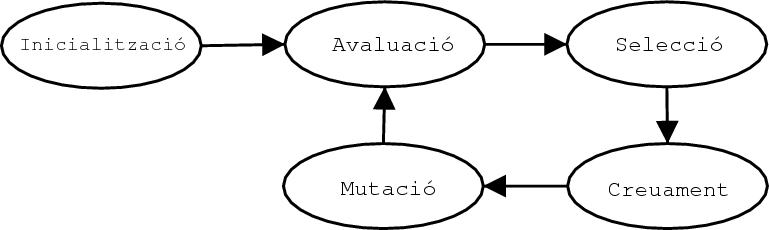
\includegraphics[width=4in]{intro/ga}
\caption{\label{fig:ga}Diagrama d'activitats d'un algorisme genètic}
\end{figure}

A grans trets, la fase d'inicialització, crea la població inicial que començarà
el procés evolutiu. Sempre cal un conjunt suficientment gran i divers per
assegurar l'èxit del procés evolutiu \cite{G02}.

Pel que fa a l'avaluació, cal dir que és un dels aspectes més importants d'un
GA, en l'apartat \ref{subsec:avaluacio} s'entrarà amb molt més detall amb aquest
afer, però cal comentar abans que la funció d'avaluació és en si mateix el
problema que es vol resoldre o optimitzar.

La selecció és el mecanisme que tria els individus que seran candidats a ser
escollits, més endavant s'entrarà en molt més detall en els mecanismes
involucrats en la selecció desenvolupada, i també es citaran altes tècniques de
selecció.

El creuament és el procés pel qual es combinen dos cromosomes que s'han
seleccionat per tenir descendència. Hi han moltes formes de fer-ho, però una de
les més habituals és un creuament discret amb un o dos punts de tall.  Aquesta
és la tècnica que hem usat en dos dels nostres projectes \texttt{Pholus} i
\texttt{Chiron}  %% refs

Finalment, vé la mutació, que és l'encarregada d'introduir o canvis aleatoris en
els individus amb una probabilitat més aviat baixa. Aquesta activitat és
realitza per estar segurs de que tot l'espai de cerca pugui ser explorat.
Modificant la probabilitat d'aparició de mutacions donem més o menys
variabilitat genètica al algorisme, afavorint o desfavorint la convergència de
la població.

En acabar la mutació el cicle es tanca, i va iterant fins que la condició
d'aturada s'assoleix. Normalment la condició d'aturada és generar un nombre
prefixat de generacions, però alguns cops també s'utilitzen criteris, com per
exemple la convergència de la població.

\subsubsection{La funció d'avaluació\label{subsec:avaluacio}} La funció
d'avaluació és vital per un algorisme genètic. Aquesta tracta de simular
l'entorn en el qual estan immerses les solucions, i ens retorna el
\emph{fitness} o el grau d'adaptació dels individus a l'entorn. Cal fer notar
que la funció d'avaluació codifica el problema que es vol que el GA resolgui.

En alguns problemes la funció d'avaluació és tan complexa que s'ha de
simplificar per aproximacions més ràpides. Fins i tot en alguns casos s'ha
observat que el fet de substituir la funció d'avaluació per una menys complexa
dóna la oportunitat d'avaluar més individus per unitat de temps, i amb aquest
increment dels individus avaluats, al final s'assoleix una solució real més
acurada que la que es va trobar utilitzant la funció d'avaluació inicial
\cite{G89}. 

\subsubsection{Reproducció} En la reproducció estan implicats dos dels tres
pilars fonamentals dels GA, la selecció i el creuament. La creació de nova
descendència és un factor crític, en la mesura que de generació en generació,
els nous individus creats van superant als seus ascendents.

A partir d'ara entra en joc el concepte de pressió selectiva. És a dir, la
pressió que d'alguna manera s'exerceix sobre la població per a que vagi
augmentant el seu grau d'adaptació a l'entorn. Sovint s'ha de vigilar amb la
pressió selectiva, per que si és massa elevada, l'algorisme no té altra
escapatòria més que arribar a solucions bones a curt termini però que no
assoleixen els màxims globals. Aquestes solucions queden estancades en màxims
locals. D'altra banda si la pressió selectiva és molt baixa, el temps de
convergència és molt llarg.  Com sempre, s'ha d'arribar a un nivell de
compromís, entre el temps de convergència i el risc de caure en màxims locals.

Cal fer notar que de vegades podria ser que alguns individus siguin seleccionats
repetits cops en una mateixa generació. Això no té per que ser dolent, ja que
normalment aquests tipus d'individus tindran un \emph{fitness} molt alt.

Quan els individus que van a ser creuats ja han estat seleccionats, sols queda
pendent emparellar en grups de dos els individus per tal de generar nova
descendència. 

Un concepte que també s'ha d'introduir és el concepte d'\texttt{elitisme}, que
implica guardar els $k$ millors individus de la població de generació en
generació, així s'assegura que els millors individus de la població no es perden
mai.  Aquest és un element que afegeix pressió evolutiva, mantenint un ``llistó''
del que no es baixa mai generació a generació, i accelerant la convergència.

\subsubsection{Convergència} 

Normalment els individus d'un GA van convergint cap als màxims de la solució de
generació en generació. Es diu que un GA ha convergit quan el 95\% de la
població té el mateix valor \cite{D75}, i una població ha convergit quan tots
els seus gens han convergit.

En alguns casos la condició d'aturada del cicle d'activitats d'un GA ve imposat
per condicions de convergència.  Quan els individus han assolit un cert nivell de
convergència (el 95\% dels individus d'una generació són iguals), en general
implica que el GA no evolucionarà més les solucions, per tant té sentit aturar
la cerca.

Quan apliquem operadors (veure secció \ref{subsec:operadors}) molt restrictius,
que donen molta pressió evolutiva, ens podem trobar en casos de
\emph{convergència prematura}, és a dir, en poques generacions, tots els
individus s'assemblen massa entre ells i els creuaments són poc efectius.  En
aquests casos, l'algorisme s'estanca en un màxim o mínim local, però rarament
global.

\subsection{Operadors\label{subsec:operadors}} 

S'entenen com els operadors d'un GA com les diferents tècniques de realitzar les
5 fases bàsiques d'un GA. En el treball final de carrera titulat com
\emph{Química combinatòria virtual: disseny de pèptids que travessen la barrera
hematoencefàlica} \cite{B01},  hi ha un ampli recull d'operadors, on s'analitzen
els punts forts i febles de cadascun.  A continuació es descriuen els operadors
emprats en el GA desenvolupat en aquest projecte en cadascuna de les fases.

\subsubsection{Inicialització} 
\label{ssub:IInicialitzacio}

Per fer les inicialitzacions es poden descriure molts mètodes, des de models
totalment aleatoris, fins a la incorporació de certes heurístiques o coneixement
sobre el problema. En aquest projecte s'ha optat per una inicialització
aleatòria, sempre i quan els cromosomes compleixin amb els requeriments del
problema.  Com s'explica en cadascun dels apartats, cada gen pot prendre un
nombre finit de valors, o com a màxim, un rang (en el cas de ser representat per
un real).

\subsubsection{Selecció}
\label{subs:Iseleccio}
La selecció és la manera en que s'escolliran els individus de la població més
ben adaptats, per a permetre que aquests siguin els ``pares'' dels individus de
la següent generació.

La selecció, en els algorismes evolutius és típicament probabilística, donant
més probabilitats de ser ``pares'' als cromosomes de més qualitat que als de
menys.  De totes maneres, els individus de poca qualitat també tenen alguna
possibilitat d'encreuar-se i així passar el seu ``codi genètic'' a generacions
futures.

Tècniques de selecció n'hi ha moltes, i aquí n'explicarem només algunes, les
que hem provat per als nostres projectes, o bé alguna d'especialment curiosa.

Els \emph{fitness proportional selection}, també anomenat selecció per ruleta
basen el seu funcionament en què per a cada selecció, la probabilitat que un
individu $f_i$ sigui seleccionat per a reproduir-se depèn únicament del seu
\emph{fitness} absolut comparat amb els fitness dels altres individus de la
població (Figura \ref{fig:rwsgraph}).

Aquest mecanisme de selecció va ser introduït a \cite{H75} i ha estat molt
estudiat en endavant.  Donada la seva simplicitat, s'han trobat diversos
problemes:

\begin{itemize}
	\item Els individus que són molt més bons que la resta, tendeixen a
	``conquerir'' la població sencera molt ràpidament. Provoca convergència
	prematura.
	\item Si els fitness dels individus són molt similars, la pressió selectiva
	es veu molt mermada, fent que a la hora d'escollir, es tingui gairebé les
	mateixes probabilitats d'escollir un individus que un altre, fent que la
	selecció segueixi una distribució uniforme aleatòria.
\end{itemize}


\begin{figure} \centering 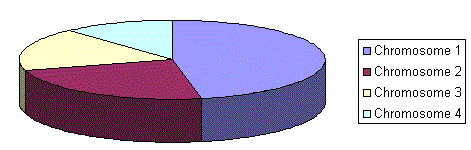
\includegraphics[width=4in]{intro/rwsgraph.png}
\caption{\label{fig:rwsgraph}Ruleta FPS}
\end{figure}

La selecció \emph{basada en ranking}, és un altre mètode que intenta
solucionar els problemes de FPS \cite{B87a}.  Aquest mètode manté la pressió
selectiva ordenant la població en funció del seu fitness, i assignant les
probabilitats de selecció en funció de la ordenació en comptes de fer-ho en
funció del propi fitness. D'aquesta manera, s'estableix una relació de qui és
millor que qui, però no hi ha els problemes que teníem en FPS.  El problema que
té aquest mètode és que no fa cap distinció entre les relacions de fitness
excepte per la relació de ser millor que un altre.  Per exemple, tres elements
amb fitness 1,2,3 s'ordenaran igual, i amb les mateixes probabilitats de ser
seleccionats que elements amb fitness 1,100 i 1000 .  La manera que es té de
mitigar (que no solucionar) aquest problema és assignar proporcions escalades en
relació entre la posició en el ranking i la probabilitat de ser seleccionat,
pot ser una relació lineal, exponencial o bé logarítmica. 

En la figura \ref{fig:rank1} es mostra  un cas on hi ha un cromosoma que tindria
el 90\% de probabilitats de ser escollit. El que es fa és ordenar de pitjor a
millor, i al pitjor donar-li un ``calaix'', al següent dos, al següent tres, i
finalment, al millor quatre. 

\begin{figure} \centering 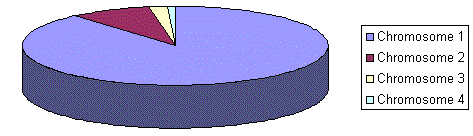
\includegraphics[width=4in]{intro/rank1.png}
\caption{\label{fig:rank1}selecció ranking}
\end{figure}

En casos reals, s'utilitzen sistemes una mica més sofisticats, com per exemple
la \emph{selecció per torneig}.  En una selecció per torneig s'ha de definir
un paràmetre $N$ que descriu la mida del torneig.

En la selecció per torneig, per decidir quin individu passarà a la següent
generació, es realitzen ``enfrontaments'' de $N$ individus, comparant el seu
fitness.  El que guanya de tots ells serà qui passarà a la fase de creuament.

Una de les avantatges que té aquest mètode és que no fa falta tenir
comptabilitzats tots els fitness de la població sencera, ja que només s'han
d'avaluar per grups de $N$.  Això el fa molt còmode d'usar en sistemes
paral·lelitzats, o bé en problemes on es molt costós fer una ordenació dels
fitness a nivell global, com per exemple, quan avaluem tirades en un joc
estratègic.

Hi ha variants de tornejos on, es defineix un altre paràmetre, que és la
probabilitat que el que té millor fitness surti realment guanyador.  En els
tornejos normals (deterministes), aquest paràmetre $p=1$, però si el disminuïm
tal que $p<1$, hi haurà un numero de casos $1-p$ on no guanyarà el millor.
Aquesta tècnica redueix la pressió evolutiva permetent que individus pitjors,
passin el seu codi genètic a següents generacions, augmentant la diversitat.

L'algorisme esquematitzat (tant per p=1 com per p<1) és el següent:

\begin{itemize}
	\item S'escullen $N$ individus de la població aleatòriament.
	\item S'agafa el millor individu amb probabilitat $p$.
	\item S'agafa el segon millor individu amb probabilitat $p \times (1-p)$
	\item S'agafa el tercer millor individu amb probabilitat $p \times (1-p)^2$
	\item \ldots
\end{itemize}


%En aquest projecte s'ha utilitzat una selecció \emph{stochastic
%universal samplig} \cite{B87a} amb \emph{rank selection} \cite{B87b} i una
%tècnica d'especiació coneguda com \emph{sharing} \cite{33}.

\subsubsection{Creuament}

Un cop s'han seleccionat els individus de la nova població, aquests podran tenir
descendència. Per a cadascun d'ells es genera un nombre aleatori entre 0 i 1, i
si no supera una determinada probabilitat de creuament, normalment bastant alta,
és copiat directament a la següent fase que és la mutació.

Els individus escollits per creuar-se són agrupats en parelles aleatòries, i
s'aplica un creuament clàssic discret unipunt.  Es genera un punt de tall del
cromosoma de forma aleatòria, i es construeixen dos descendents. El primer
descendent contindrà la primera part del material genètic del primer progenitor
fins el punt de tall, i la segona part del segon progenitor, que va des del punt
de tall fins el final del cromosoma. El segon descendent serà a l'inrevés, la
primera part serà directament la primera part del segon progenitor, i la segona
part la segona del primer progenitor.

En els dos problemes de GA hem utilitzat el creuament unipunt, però també hi
ha variants d'aquest creuament utilitzant dos o més punts.  Com es veurà en les
seccions de cadascun dels problemes, s'han fet proves amb aquests creuaments,
però no ens han donat resultats millors, i hem seguit amb els creuaments
unipunt.

Aquests creuaments, es poden aplicar amb seguretat quan considerem que la
relació d'un gen $i$ amb el gen $i+1$ no és forta (no hi ha epistàcia).  Si
trencant un cromosoma per la posició $i$, destruïm algun \emph{building block},
probablement, es perdrà un factor que feia que l'individu fós bo, i al
creuar-lo, no obtindrem gaire bons resultats.

\subsubsection{Mutació}

Finalment, abans de tancar el cicle, es realitza la mutació. Aquesta activitat
aplica mutacions de forma aleatòria, però amb una baixa probabilitat, als gens
dels individus de la nova generació que està a punt de crear-se. En el cas de
disposar d'elitisme, aquests individus no són exposats a les mutacions.

L'operador de mutació emprat és clàssic uniforme. Això implica que els gens
seleccionats per a ser mutats, se'ls canvia el seu valor de forma aleatòria
però, el nou valor pertany al domini de la variable de decisió que codifica
aquell gen.

\subsubsection{Reemplaçament}

El model de reemplaçament seleccionat és el conegut com elitisme, que com ja
s'ha explicat abans, crear tota una nova població d'individus de generació en
generació. Malgrat això els $k$ millors individus van guardant-se per tal
d'assegurar que no es perden al llarg del procés evolutiu.  En tots els
projectes que es presenten en aquest treball, s'ha mantingut la mida de la
població, però també es possible fer que aquesta mida de la població varii al
llarg de les generacions.

%\subsection{Teoremes} En general no n'hi ha cap teoria universalment acceptada
%del perquè funcionen bé els GA, ni del perquè de la seua robustesa. Però n'hi
%han dues hipòtesis que són interessants conèixer per que ens poden ajudar a
%implementar bones aplicacions dels GA, i cada cop més estan adoptant-se pels
%teòrics com els vertader mecanismes que fan evolucionar els GA. El primer
%d'ells és el teorema de la disposició, i el segon la hipòtesi dels blocs de
%construcció, o \emph{building blocks}.

%\subsubsection{Teorema de la disposició} Més conegut per \emph{schema theorem},
%va ser proposat per Holland \cite{H75}. Un \emph{schemata} és un patró de
%valors dels gens en binari. On aquest patró està format \{1, 0, \( \star  \)\}
%sent \( \star  \) el caràcter comodí. De tal forma que cromosomes com
%{}``0000'', {}``0010'', {}``0001'' i {}``0011'' corresponen al mateix patró
%{}``00\( \star \star  \)''.

%Aquest teorema diu que els individus bons, ho són per que tenen un bon patró.
%Llavors hem de donar-los a aquests individus més possibilitats de reproducció
%en funció del seu \emph{fitness}.  Per tant al passar aquests patrons a la
%descendència i al aplicar-los aquest mateixa filosofia, anem augmentant les
%possibilitats de generar millors patrons a mesura que passa el temps.

%Segons Holland si distribuïm aquestes probabilitats en funció de la proporció
%del \emph{fitness} d'un individu a seleccionar front al de la resta, un bon
%patrons estarà tenint un nombre de possibilitats que va creixent
%exponencialment. També va dir que el nombre de patrons que estant sent
%processats en una generació, és n\( ^{3} \), on n és el tamany de la població.
%Això és conegut com paral·lelisme implícit.

%\subsubsection{Hipòtesi sobre els blocs de construcció \label{subsec:bb}}
%Goldberg, en canvi, formula la \emph{Building Block Hypotesis} \cite{G89}.  Que
%diu que la potència dels GA's recau sobre l'habilitat de crear bons blocs de
%construcció. Aquests són curts patrons amb una longitud fixa, que funcionen
%molt bé per separat; independentment de la resta del cromosoma. I que si se li
%és incorporat un bon bloc de construcció a un cert individu, el seu
%\emph{fitness} augmenta. 

%Per afavorir la aparició de blocs de construcció, la codificació del cromosoma
%hauria de tenir propers els gens relacionats, i al mateix temps, que la
%interacció entre els gens siga mínima.

%La no interacció entre gens vol dir que l'aportació d'un gen al còmput del
%\emph{fitness} no es vegi afectat per els valors que poden prendre altres gens.
%Més tard Goldberg va publicar els estudis teòrics sobre gens que sí que
%interaccionen entre ells i com aprendre aquestes interaccions
%\cite{Goldberg:2002}, això és conegut com \emph{linkage learning}, i amb
%l'algorisme BOA que en la secció \ref{EDA} s'explicarà, es poden arribar a
%salvara aquest tipus d'inconveniències. Cal dir que en aquest projecte el
%còmput del \emph{fitness} si que s'espera que es veja afectat per la
%interrelació entre gens.

\section{Programació d'expressions genètiques} % (fold)
\label{sec:Programacio d'expressions genetiques}

La programació d'expressions genètiques (GEP), podríem dir que és una evolució de
la programació genètica (GP) en tant que intenta solucionar el mateix tipus de
problema.  A diferència dels GA clàssics, que tracten de solucionar (al menys de
forma natural) problemes d'optimització, tant GP com GEP podríen ser
classificats dins dels algorismes d'aprenentatge.  Per posar un exemple, en la
majoria de GA, el que es busca optimitzar és una entrada per a un procés
(Figura \ref{fig:ch1-4}).  En canvi, en GEP i GP el que es busca és un procés que
optimitzi una entrada donada (Figura \ref{fig:ch1-5}).

\begin{figure} \centering 
\includegraphics[width=4in]{intro/1-4.jpg}
\caption{\label{fig:ch1-4}Optimització d'entrada}
\end{figure}
\begin{figure} \centering 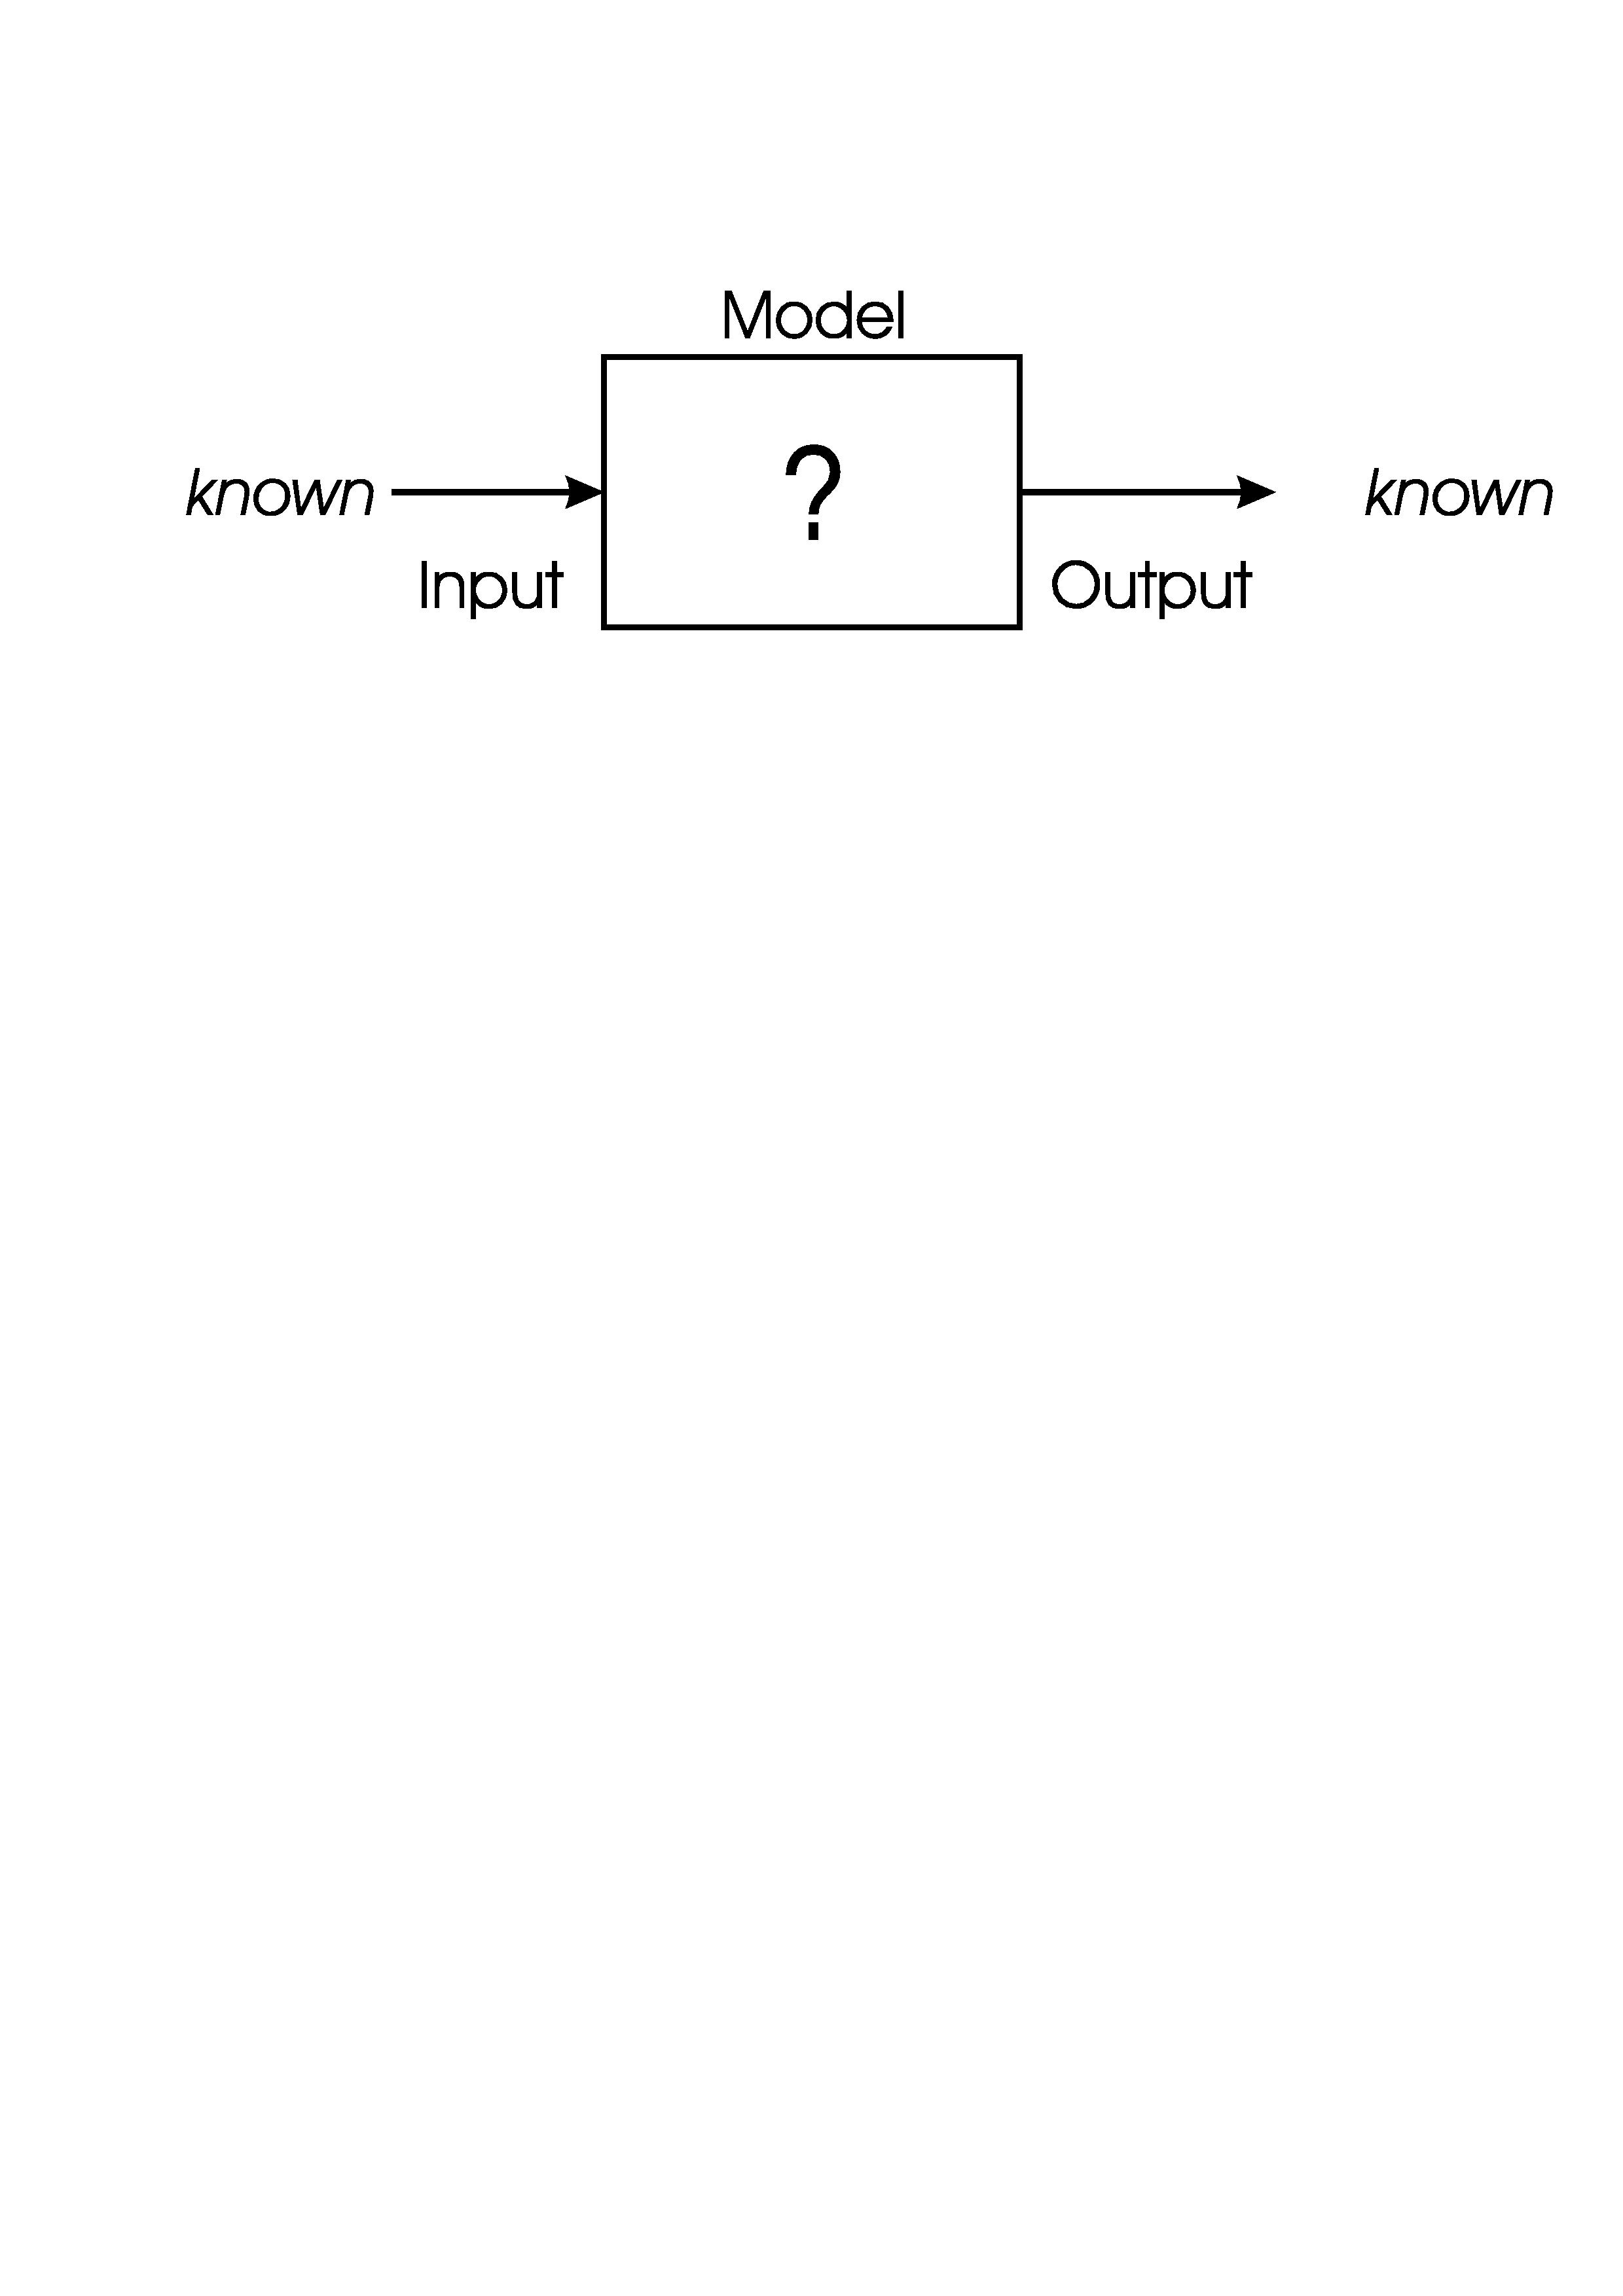
\includegraphics[width=4in]{intro/1-5.jpg}
\caption{\label{fig:ch1-5}Optimització procés}
\end{figure}

Els processos que s'intenten optimitzar, contenen, és clar, molta més informació
que en un dels algorismes genètics dels que s'han vist fins ara.  Això és
evident, ja que aquí, els individus són parts funcionals d'un sistema i no
només dades que un sistema agafarà i avaluarà.  Tot seguit es mostren tres
exemples de possibles problemes que es poden optimitzar:

\begin{itemize}
	\item Fórmules lògiques (per exemple $ (x\land true) \rightarrow ((x \lor y)
		\lor (z \leftrightarrow ( x \land y)))$ ). Figura \ref{fig:6-2-2}.
	\item Fórmules aritmètiques (per exemple $2\times\pi+((x+3)-\frac{y}{5+1})$
		).  Figura \ref{fig:6-2-1}
	\item Programes 
		\begin{verbatim}
				i = 1;
				while (i<20){
					i = i + 1;
					}
		\end{verbatim}. Figura \ref{fig:6-3}.
\end{itemize}

\begin{figure} \centering 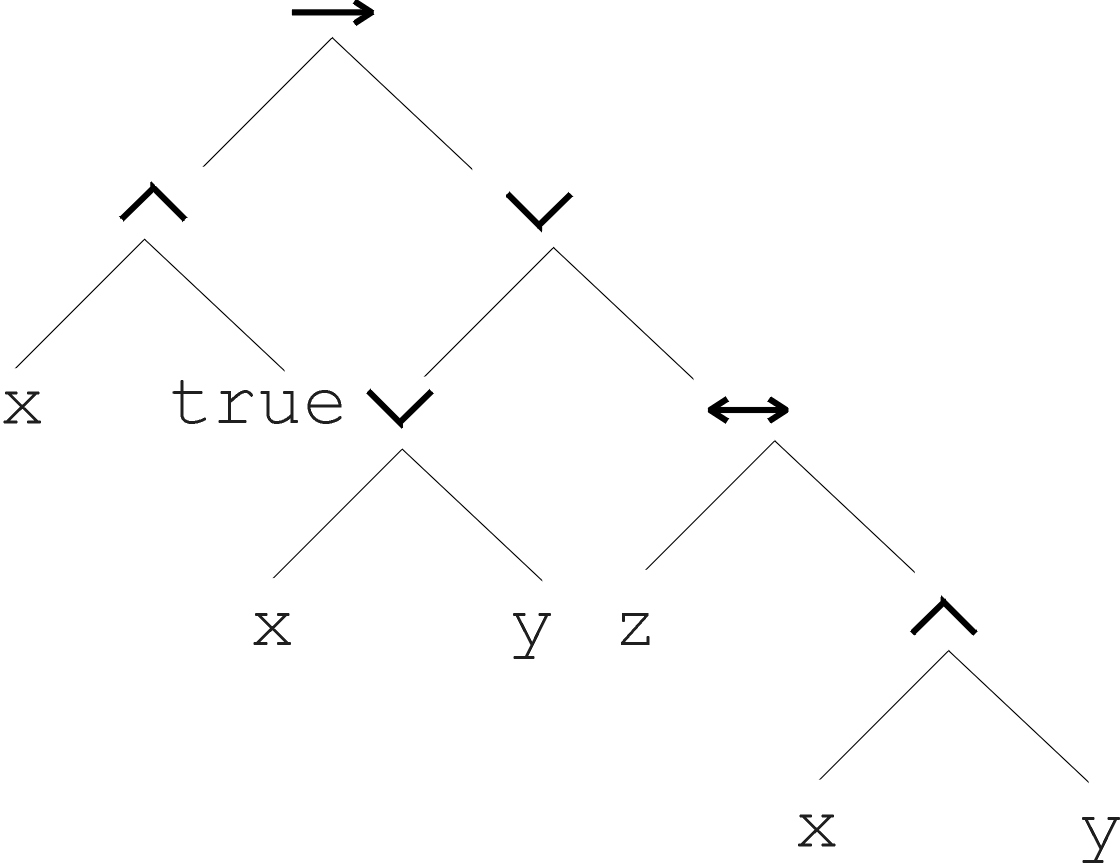
\includegraphics[width=4in]{intro/6-2-2.jpg}
\caption{\label{fig:6-2-2}Fórmula logica}
\end{figure}

\begin{figure} \centering 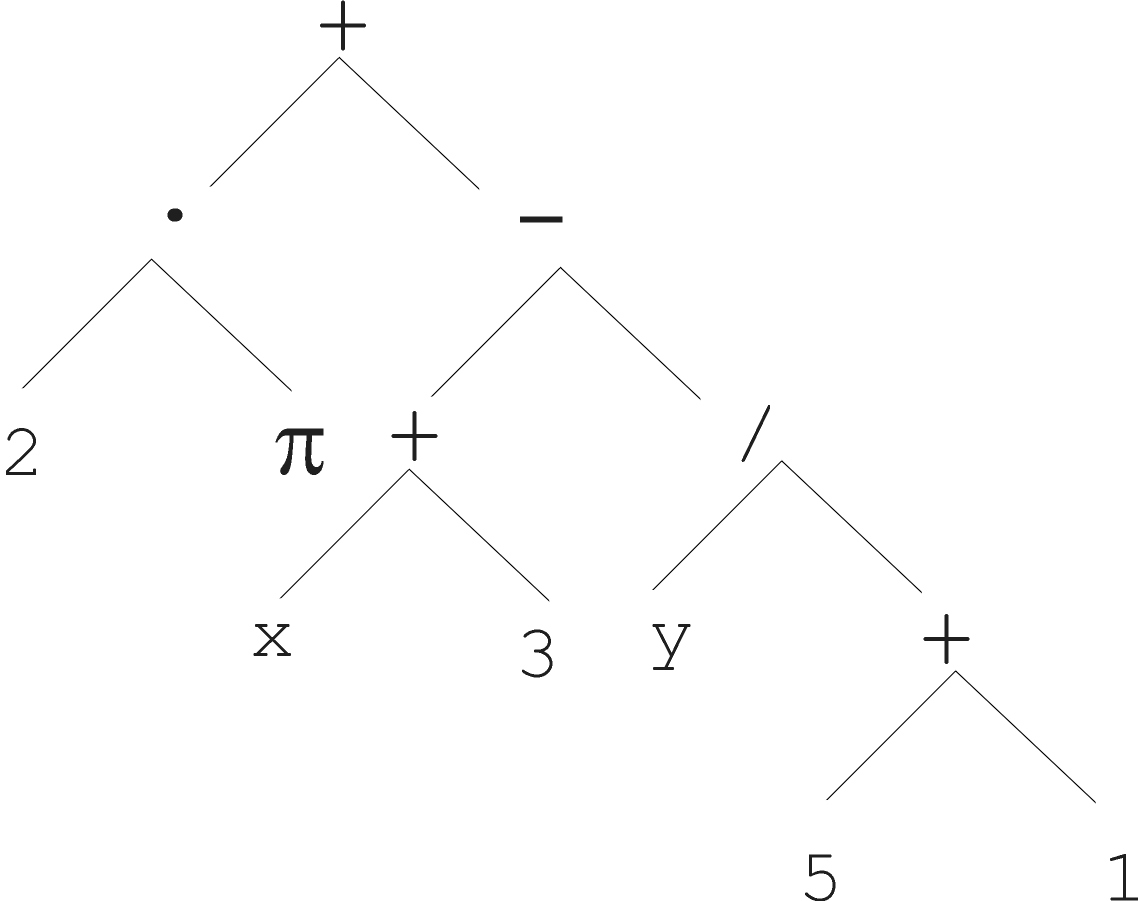
\includegraphics[width=4in]{intro/6-2-1.jpg}
\caption{\label{fig:6-2-1}Fórmula aritmètica}
\end{figure}

\begin{figure} \centering 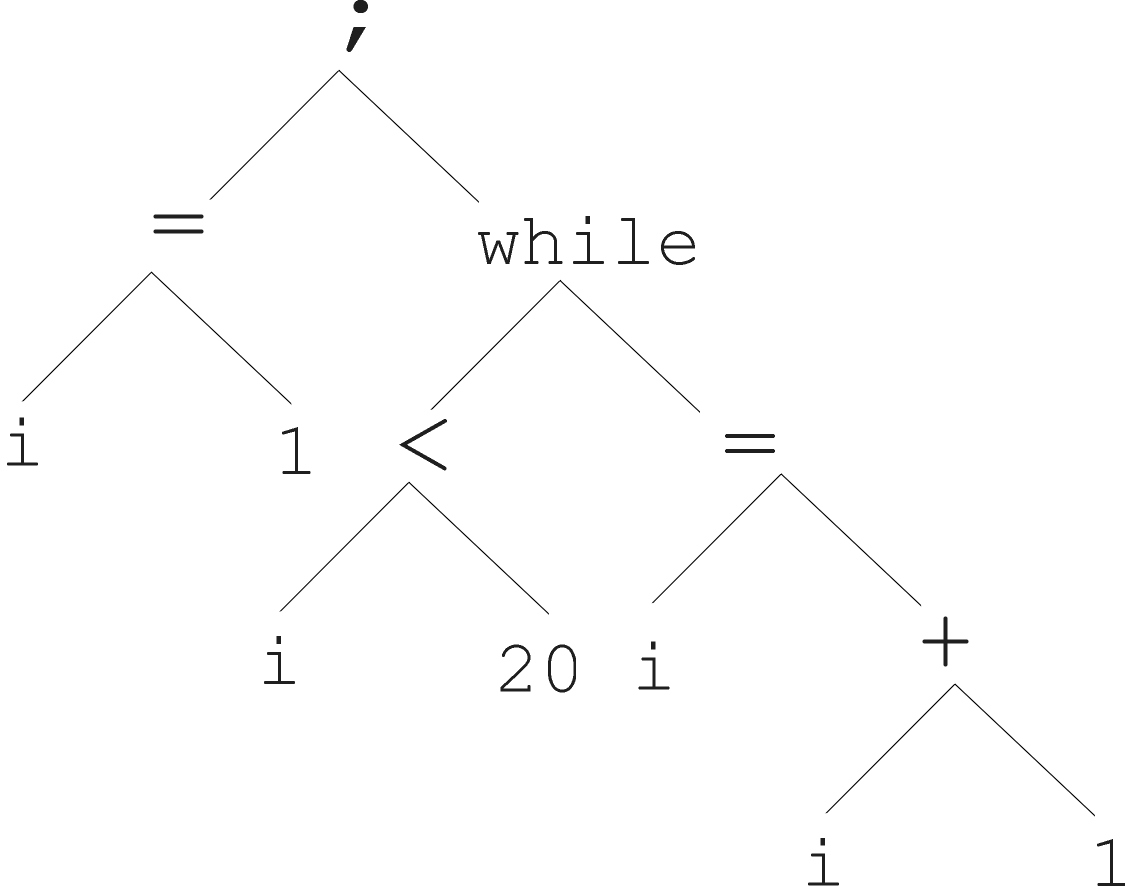
\includegraphics[width=4in]{intro/6-3.jpg}
\caption{\label{fig:6-3}programa}
\end{figure}

En aquest tipus d'algorismes, els individus no poden ser codificats com a un
sol vector de bits o reals, i aquests ser tractats independentment uns dels
altres, sinó que el que han de codificar els individus són arbres.  Per tant,
la seva codificació és més complexa, havent-hi una clara separació entre genotip
i fenotip.

Estrictament parlant, però, no hi ha cap altra diferència entre els GA clàssics
i GP o GEP.  Simplement, aquí interpretem els cromosomes com a arbres.

A continuació es farà una breu introducció a GP, per saber els orígens de
GEP, i seguirà una explicació una mica més detallada de GEP, que és la tècnica
que s'ha utilitzat en \texttt{GEP}.

\subsection{Antecessors: Programació Genètica} % (fold)
\label{sub:Ant. Programacio Genetica}
La programació genètica és una de les diferents disciplines dins dels algorismes
evolutius, inventat per Cramer en el 1985 (\cite{C85}) i després millorat per
Goldberg (\cite{Goldberg:89}) i
John Koza en 1992 (\cite{koza:92}) basat en la solució de problemes amb genotips de
llargada fixa, però interpretats de forma no lineal (arbres) de mida i formes.

Els individus en GP, normalment tenen un alfabet més ric que els algorismes
evolutius clàssics, però aquesta riquesa que ofereix tractar els cromosomes amb
una interpretació no lineal, fa que aquests individus no siguin autònoms, i no
poden funcionar com a genotip i fenotip alhora, ja que han de passar per una
fase de ``traducció''.

Per poder diferenciar la programació genètica de la programació d'expressions
genètiques, fem un repàs molt ràpid dels operadors més comuns en GP.

\subsubsection{Operadors} % (fold)
\label{ssub:operadors}

Els algorismes de programació genètica tenen els mateixos operadors que els
altres AE, però amb la diferència notable que s'ha de tenir en compte que al fer
una modificació sobre el genotip, el fenotip pot veure's modificat de manera
``no prevista'' si no anem molt en compte.  Per exemple, al fer un creuament
entre dos individus, el cromosoma resultant, pot no mantenir cap (o gairebé
cap) característica dels seus pares, donada la no-linealitat dels fenotips
respecte els genotips.  Això dona lloc a que molts dels individus generats a
partir de individus vàlids, són invàlids en el sentit que poden no complir les
condicions bàsiques per a ser traduïts a fenotips i posteriorment avaluats.

Una manera de assegurar que les propietats dels progenitors es mantenen a la
descendència i que continuen essent individus vàlids, és aplicar els operadors
a nivell de fenotip, i assegurant-se que els fills continuen tenint una mínima
entitat que els fa avaluables en el context del problema.  Això dificulta molt,
però, la programació dels operadors.

Per exemple, en el cas d'interpretar els genotips com a arbres amb formules
matemàtiques, al fer creuaments podem fer-los per subarbres, agafant l'arrel i
el fill esquerra del arbre d'un dels dos progenitors, i el fill dret de l'altre.
Tot seguit es comenten els dos operadors més interessants en programació
genètica.

\paragraph{Mutacions} % (fold)
\label{par:Mutacions}
Les mutacions en programació genètica són similars conceptualment a les que
trobem en els altres algorismes evolutius, canviant un subarbre aleatori del
cromosoma per un altre subarbre generat aleatòriament.  Veiem aquí la diferència
necessària en la implementació, ja que la mutació té lloc en l'espai del fenotip
(arbre) i no pas en el genotip (vector de símbols).  Hi ha hagut controvèrsia
sobre la aplicació de mutacions en programació genètica des de els seus inicis.
Koza en \cite{koza:92} aconsellava desactivar per complet la mutació.   Més
endavant, s'ha anat donant una mica més importància, però sense ser mai un
operador fonamental, donat que el creuament també actua en certa manera
d'operador de mutació però a més gran escala.  Aquestes mutacions canvien la
mida dels cromosomes.
% paragraph Mutacions (end)

\paragraph{Creuament} % (fold)
\label{par:Creuament}
El creuament de cromosomes en programació genètica és un operador binari que
consisteix en intercanviar dos subarbres entre dos cromosomes d'una població.
Una altra vegada, perquè el creuament no doni lloc a elements sintàcticament
incorrectes, el creuament s'ha de realitzar a nivell d'arbre, provocant també
canvis en la mida dels cromosomes.

% paragraph Creuament (end)

% subsubsection operadors (end)
% subsection Ant. Programació Genètica (end)

\subsection{Principis bàsics} % (fold)
\label{sub:Principis Basics}

La programació genètica, però, té alguns problemes fonamentals, que mermen la 
seva potència, com són el sobreentrenament (és molt fàcil obtenir 
solucions sobreentrenades per al conjunt de mostres amb el que entrenem
 l'algorisme), el \emph{bloat} (els arbres, tendeixen a créixer desmesuradament),
o bé la mateixa complexitat que té fer els creuaments o mutacions a nivell de 
fenotip. GEP, intenta solucionar alguns d'aquests problemes.


En GEP, els principals elements son els cromosomes i els arbres d'expressions,
on els segons són la expressió del la informació genètica codificada en els
cromosomes.  Com en la natura, el procés de descodificació s'anomena
\emph{traducció}.

La correspondència d'un a l'altre ha de ser unívoca i hi ha unes regles que ens
permeten passar d'un a l'altra.  En la natura, aquesta traducció no és pas tant
fàcil, ja que no se sap gairebé res del genotip, si tenim només un fenotip, però
per a tenir una traducció fàcil dins de GEP, es disposa d'una notació anomenada
\emph{Karva Notation} que ens permet fer les traduccions en les dues direccions
fàcilment \ref{ssub:Notacio Karva}.

% explicar constants


%http://www.gene-expression-programming.com/Tutorial002.asp
\subsubsection{Notació Karva} % (fold)
\label{ssub:Notacio Karva}

La notació Karva, és una manera de representar qualsevol expressió matemàtica o
lògica en una estructura lineal de manera que es pugui traslladar a un arbre
fàcilment \cite{ferreira:2001} i \cite{ferreira:2006}.

Les estructures lineals que conformen els individus en GEP són els cromosomes,
i cada cromosoma té un o més gens, que aquí prenen un altre significat més
ampli, no referint-se als ``àtoms'' indivisibles (com en els AE que hem vist
fins ara) sinó que cada gen està associat a una K-expression.
\cite{ferreira:2007}

Tot seguit es mostra un exemple d'un gen, i en \ref{fig:expression tree1} el seu
\texttt{Arbre d'expressió} equivalent

\begin{verbatim}
0123456    
+/*abcd
\end{verbatim}

\begin{figure}[h]
\begin{center}
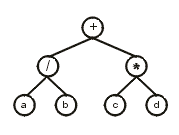
\includegraphics{intro/et1.png}
\end{center}
\caption{Arbre d'expressió}
\label{fig:expression tree1}
\end{figure}

La traducció d'un a l'altre és directe.  El primer element en el gen (posició
0) correspon a la arrel del arbre.  Llavors, sota d'aquest node, s'enganxen
tants nodes fills com arguments tingui la funció representada pel node arrel
(dos en aquest cas). Els nodes fills es van omplint recursivament, consumint
símbols del cromosoma, fins que un nivell del arbre queda només omplert per
nodes terminals, que no son més que nodes on el símbol que contenen té aritat
zero.

Més formalment, tant el gen com l'arbre \ref{fig:expression tree1} poden ser
representats per la expressió matemàtica:

	$\frac{a}{b}+c \times d$

Per assegurar que els arbres que es creïn siguin sintàcticament vàlids, es
divideix un gen en dues parts, amb mides que segueixen unes normes determinades
que s'expliquen en detall en l'apartat \ref{ssub:Inicialitzacio}.  Un gen es
composa de la primera part (\emph{head}) que conté funcions i terminals, i d'una
segona part (\emph{tail}) que només conté terminals (aritat zero). Si el tail és
suficientment llarg com per omplir la última capa del arbre que genera el propi
gen, sempre hi haurà prou operands per a donar a les funcions.

% subsubsection Notació Karva (end)

\subsubsection{Individus} % (fold)
\label{issub:individus}
% subsubsection individus (end)

Com s'ha explicat en \ref{ssub:Notacio Karva}, els individus son representats en
una tira de símbols (genotip), però al interpretar-los i avaluar-los, tenen una
representació en forma d'arbre d'expressió similar a un AST\footnote{Abstract
syntax tree}.

Un individu o cromosoma està format per un o més gens.  En la versió més
primària, un cromosoma conté només un gen, però es poden combinar diversos gens,
creant cromosomes multigen, com s'explicarà més endavant.

En aquest tipus de notació, existeixen el que denominem ``zones
no-codificadores'', que són parts del gen, que per diversos motius formen part
del genotip, però no tenen representació, ni es mostren en el fenotip.  Un
exemple d'això és


\begin{verbatim}
	01234567890123456 	 
	Q/a*+b-cbabaccbac
\end{verbatim}

On la $Q$ representa l'arrel quadrada.  En aquest gen, té el i \emph{head} (que ocupa
de la posició 0 a la 7) de llargada, i el tail (de la 8 a la 16) de llargada 9.
El head té tan funcions com terminals, i el tail, només té terminals.

La codificació d'aquest gen es mostra en \ref{fig:unfinished} mostra com en aquest cas,
no han fet falta tots els elements del gen per a construir l'arbre.  Això és
perquè la fórmula que en assegura tenir prou tail, preveu el pitjor dels casos,
essent tots els elements del head funcions amb la màxima aritat.  Com que en
aquest cas, tenim una arrel quadrada (i en l'arrel del arbre), deixem de
necessitar gairebé la meitat del gen per a fer la traducció.

\begin{figure}[h]
\begin{center}
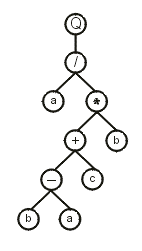
\includegraphics{geptut/pt02.png}
\end{center}
\caption{Arbre d'expressió}
\label{fig:unfinished}
\end{figure}

Aquests trossos de cromosoma que no s'utilitzen, participen igualment en els
creuaments (es fan a nivell de vector de símbols), i fan que una mutació en una
zona del \emph{head} ``activi'' una zona prèviament inactiva.  Això dona tant
als creuaments com a les mutacions molta més versatilitat que en els algorismes
clàssics.

Aquesta elegància de la programació d'expressions genètiques és la clau del
funcionament de GEP.  La codificació Karva és el nucli del bon funcionament de
GEP, però és només el principi.  És a dir, existeixen mètodes més avançats que
parteixen d'aquesta base, i aconsegueixen millorar els resultats del GEP
estàndard, com per exemple, codificar més d'un gen en un cromosoma. Són els
anomenats cromosomes multigen.  En aquests sistemes, els cromosomes estan
codificats a partir de diversos gens, i cadascun d'ells formen un subarbre o
subprograma.  Una vegada traduïts cadascun dels subarbres, aquests poden ser
connectats entre ells de diferents maneres.  Una de les més utilitzades és usant
funcions especials, anomenades d'enllaç. Aquestes funcions uneixen linealment
els diferents subarbres per ordre d'aparició en el gen.  Per exemple, observem
el següent cromosoma, composat per tres sub-gens.
	%XXX

	\begin{center}
	\begin{verbatim}
	012345678012345678012345678 	 
	*aQ+abbaa/Q*/aababa*+Qaabba
	\end{verbatim}
	\end{center}


Aquest cromosoma codifica tres arbres de la Figura \ref{fig:tres sub-et}

\begin{figure}[h!]
\begin{center}
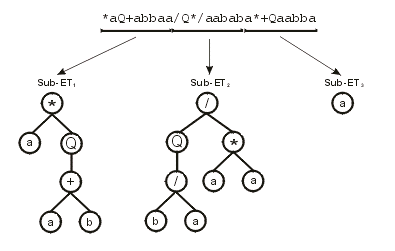
\includegraphics{geptut/pt03a.png}
\end{center}
\caption{Cromosoma representant tres sub-arbres}
\label{fig:tres sub-et}
\end{figure}

Si s'utilitzen funcions d'enllaç, per exemple, la suma, la avaluació del
cromosoma complet passaria a ser el mostrat en la figura 
\ref{fig:tres sub-et amb link}

\begin{figure}[h!]
\begin{center}
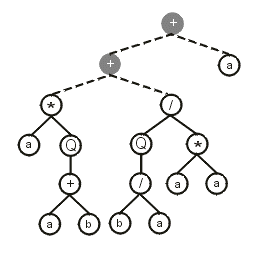
\includegraphics{geptut/pt03b.png}
\end{center}
\caption{Representació dels tres sub-arbres enllaçats amb la operació suma}
\label{fig:tres sub-et amb link}
\end{figure}

La implementació del individu que hem programat ha estat una versió una mica més
avançada que la de les funcions d'enllaç, que utilitza un dels subarbres, com a
metadada, on els terminals no es refereixen a terminals de la funció, sinó que
són referències als altres subarbres, que sí tenen com a fulles les entrades de
la funció objectiu.

%XXX
%\subsubsection{Esquema Bàsic} % (fold)
%\label{ssub:Esquema Basic}
%% subsubsection Esquema Bàsic (end)

%\subsubsection{Funció d'avaluació} % (fold)
%\label{ssub:funcio d'avaluacio}
%% subsubsection funció d'evaluació (end)
%% subsection Principis Bàsics (end)

\subsection{Operadors} % (fold)
\label{sub:Operadors}

Tot seguit es descriuran els operadors usats en GEP, sense concretar la seva
implementació, sinó explicant com varien els individus.  Per a veure els
detalls sobre la aplicació en aquest projecte, les explicacions i
implementacions més complertes consultar la secció \ref{cha:GEP}.

\subsubsection{Inicialització} % (fold)
\label{ssub:Inicialitzacio}
Donades les particularitats de la notació Karva, la inicialització d'arbres
aleatoris, consisteix en omplir head i tail amb símbols aleatoris permesos en
cadascuna de les zones.  Normalment, el head tindrà símbols operadors i
variables terminals i el tail, únicament contindrà variables terminals.  La
aritat zero dels terminals ens garantitza que l'arbre serà sintàcticament
correcte.

La població inicial es genera aplicant aquest algorisme a cadascun dels
individus.
% subsubsection Inicialització (end)

\subsubsection{Selecció} % (fold)
\label{ssub:Seleccio}
En GEP, també s'utilitza, per norma general la selecció per ruleta
(secció \ref{subs:Iseleccio}).  Un individu té una probabilitat de ser seleccionat per a
la reproducció proporcional al seu fitness en valor absolut, respecte als altres
individus de la població.

% subsubsection Selecció (end)

\subsubsection{Creuament} % (fold)
\label{ssub:Creuament}

El creuament, juntament amb la mutació és l'element que dóna la major part de la
riquesa als algorismes GEP.  Els creuaments en GEP són uns operadors que, a
diferència de la programació genètica, donen molta llibertat per a la
experimentació, ja que només s'han de mantenir unes certes regles molt bàsiques,
i es pot assegurar que es generaran arbres sintàcticament correctes.

Per exemple, en GEP es poden aplicar creuaments típics dels algorismes evolutius
clàssics, com el \texttt{creuament per un punt}, o els \texttt{creuaments per
diversos punts}, ja que si no variem la mida de la descendència, sempre es
mantindran certes les regles de què el tail no contingui mai operands (nodes
d'aritat $>0$).

A més a més, GEP té uns creuaments particulars, anomenats \texttt{recombinació
de gens}, que es basen en separar els dos individus a creuar en els seus
diferents gens, i fer el creuament ajustant els punts de tall als límits dels
gens.  Aquest creuament només és aplicable si implementem individus multigen.
% subsubsection Creuament (end)

\subsubsection{Mutació} % (fold)
\label{ssub:Mutacio}
Les mutacions, igual que els creuaments, també es poden dividir en dos
subconjunts, els que són totalment portables del món dels AE clàssics, i els
particulars de GEP.

Una mutació dels AE clàssics pot ser, per exemple, l'alteració d'un símbol
aleatori.  L'únic que s'ha de tenir en compte, és quina posició del gen s'està
mutant, per a no incloure en el tail símbols que estan restringits a usar-los
només en el head.

Per altra banda, GEP disposa de tres mutacions pròpies, anomenades IS, RIS i
``translació de gen'', que es basen en desplaçaments de conjunts de símbols al
llarg del gen.  Aquests operadors estan explicats més en detall a \ref{par:IS},
\ref{par:RIS} i \ref{par:Translacio de gen}
% subsubsection Mutació (end)

\subsubsection{Reemplaçament} % (fold)
\label{ssub:Reemplacament}

Pel reemplaçament tmabé s'utilitza elitisme, on mantenim el millor dels
individus per a la següent generació.  Les poblacions no cambien de 
mida.

% subsubsection Reemplaçament (end)
% subsection Operadors (end)
% section Programació d'expressions genètiques (end)

\section{Estat de l'art} % (fold)
\label{sec:Estat de l'art}

Actualment, els algorismes genètics estan essent més i més utilitzats no sols en
el món acadèmic, sinó també en el món de l'empresa. 


Les últimes publicacions referents a algorismes genètics tendeixen cap a
optimitzacions de la convergència.  Els algorismes genètics són processos
estocàstics (la durada o nombre d'iteracions fins a aturar-se no és un valor
conegut a priori).  Així doncs, el que s'intenta és aconseguir ``guiar''
l'algorisme perquè avanci de pressa cap a un estat convergent (s'aturi), sense
perjudicar això a la eficàcia.  Molts dels estudis de tècniques per millorar
l'eficiència dels algorismes genètics estan relacionats amb l'aprofitament de la
paralelització de processos, aprofitant sistemes distribuïts, o fins i tot en
cloud.  

Els treballs més recents relacionats amb algoritmes evolutius estan relacionats
amb la utilització de entorns de treball (frameworks) i paradigmes de
programació paralela, com poden ser hadoop o MapReduce \cite{VLCG09}.

\subsection{Tecnologia} % (fold)
\label{sub:Tecnologia}

Des dels inicis de la programació, el llenguatge per excelència
relacionat amb la intel·ligència artificial ha estat lisp \cite{JMC59}, creat per John
McCarthy el 1958 donat la gran flexibilitat que oferia (a més, en aquells temps
hi havia fortran com a alternativa, un llenguatge molt més rígid).  Així doncs,
els majors avenços relacionats amb la IA han tingut gairebé sempre les seves
primeres implementacions en Lisp o derivats (Scheme).  

El ``problema'' dels llenguatges tant dinàmics com Lisp, era que al treballar sobre
màquina virtual eren massa lents per a la implementació en producció.  Recordem que les
aplicacions que utilitzen algorismes de intel·ligència artificial requereixen un
gran volum de càlculs.

És per això que els sistemes amb grans necessitats de càlcul per a producció
normalment s'implementen amb llenguatges ``propers al ferro'' com poden ser
C/C++. 

Actualment i donada la gran potència de calcul dels ordenadors actuals, cada
vegada hi ha més empreses que comencen a utilitzar llenguatges interpretats per
a realitzar algorismes genètics. Llenguatges com Haskell i Erlang que han
demostrat ser molt ràpids i paralelitzables, no han fet el salt a la
intel·ligència artificial massivament, ja que la seva puresa (transparència
referencial i fortament tipats) els fa més ferragosos de treballar en problemes
eminentment dinàmics com els algoritmes evolutius.

% subsection Tecnologia (end)
% section Estat de l'art (end)

%\bibliographystyle{unsrt} 
%\bibliography{bibliografia}


%\end{document}


%\documentclass[a4paper]{article}
\usepackage[catalan]{babel}
\usepackage[utf8]{inputenc}
\begin{document}
La computació evolutiva és un camp recerca dins de la informàtica.  Com el nom
indica, es un camp especial dins la computació, una manera determinada d'atacar
problemes que agafa idees en la evolució natural de les espècies.  No es extrany
que s'hagin intentat portar idees de la naturalesa a camps de la computació, i
menys a camps relacionats amb la inteligència artificial, ja que és ben clar
que, la evolució en aquets cas, ha tingut un fort impacte positiu en les
espècies, a nivell individual, i als ecosistemes, amb multitud d'espècies
convivint i co-evolucionant al llarg del temps.

Un altre cas on s'intenta adaptar els procediments naturals en la computació és,
per exemple, en les ``Xarxes neuronals'', on s'intenta simular les interaccions
de les neurones en un cervell, per a solucionar problemes on hi intervé
l'aprenentatge.

fault-tolerance

En general, els problemes que la evolució intenta solucionar (la evolució no
s'atura, amb el qual mai arriba a un estadi totalment estàtic), els soluciona
mitjançant prova i error.

% TODO : Petita intro a la evolució? 

\section{Breu Història} % (fold)
\label{sec:Breu Historia}

Els principis de la aplicació de les idees de Darwin a la resolució de problemes
daten dels anys quaranta, cuan Alan Turing va proposar ``búsquedes genètiques o
evolutives''.  Al any 1962, Bremermann va executar amb èxit alguns experiments
de ``optimització mitjançant evolució i recombinació''.  Durant els anys
seixanta, es van desenvolupar diferents estudis i implementacions d'aquests
principis en 3 llocs diferents, amb 3 noms lleugerament diferents:


 % theme=Berlin;caption_top=1;caption=Els inicis
 % Nom & Qui & On
 % Fogel, Owens, Walsh & programació evolutiva & EEUU
 % & Algoritme genètic & Holanda
 % Rechenberg, Schwefel & estratègies evolutives & Alemanya

\begin{table}
\centering
\caption{Els inicis}
\begin{tabular}{|l|l|l|}
\hline
\multicolumn{1}{|c|}{\textbf{Nom }} & \multicolumn{1}{c|}{\textbf{ Qui }} & \multicolumn{1}{c|}{\textbf{ On}} \\
\hline
\hline
Fogel, Owens, Walsh  & programació evolutiva  & EEUU     \\
                     & Algoritme genètic      & Holanda  \\
Rechenberg, Schwefel & estratègies evolutives & Alemanya \\
\hline
\end{tabular}
\end{table}

Més endavant, als anys noranta, John Koza va encunyar el terme programació
genètica.  Actualment, totes aquestes variants es conceben dins del que
s'anomenen algorismes evolutius.

% TODO : Ferreira i GEP

Avui dia, i donat que les cerques en problemes NP-Complets son més i més
rellevants, les tècniques englobades dins dels algorismes evolutius estan tenint
cada any més rellevància.  Prova d'això és que ja hi ha vàries conferències
i publicacions dedicades.

\subsection{Inspiració de la Naturalesa} % (fold)
\label{sub:Inspiracio de la Naturalesa}

\subsubsection{Evolució darwiniana} % (fold)
\label{ssub:Evolucio darwiniana}

La teoria de la Evolució de Darwin \cite{Darwin} dóna una explicació de la
diversitat biològica i dels mecanismes de sel·lecció natural.  Aquesta
sel·lecció natural és qui juga el paper principal en la direcció que agafa la
evolució.  Donat un entorn que pot assumir un número limitat de individus, i
l'instint bàsic dels individus a reproduir-se, la sel·lecció esdevé inevitable.
Altrament, la població s'aniria incrementat indefinidament, i l'entorn no podria
suportar-ho.  La sel·lecció natural fa que els individus competeixin pels
recursos existents, i permet només reproduir-se als que estiguin més adaptats al
medi en qüestió.

\subsubsection{Genètica} % (fold)
\label{ssub:Genetica}

% subsubsection Genetica} (end)

% subsubsection Evolucio darwiniana (end)

% subsection Inspiració de la Naturalesa (end)

\section{Introduccio als Algorismes evolutius} % (fold)
\label{sec:Introduccio als AE}

% section Introduccio als AE (end)
% section Breu Història (end)

\section{Estat de l'art} % (fold)
\label{sec:Estat de l'art}

Actualment, els algorismes genètics estan essent més i més utilitzats no sols en
el món acadèmic, sinó també en el món de l'empresa.  Per exemplificar això, es
presenten les dades d'un article publicat a 
%XXX 

Les últimes publicacions referents a algorismes genètics tendeixen cap a
optimitzacions de la convergència, i moltes de les tècniques aprofiten sistemes
distribuits



\subsection{Tecnologia} % (fold)
\label{sub:Tecnologia}

Des dels inicis de la programació 'moderna', el llenguatge per excelència
relacionat amb la Intelligència artificial ha estat \cite{LISP}, creat per John
Macarthy el 1958 donat la gran flexibilitat que oferia (a més, en auqells temps
hi havia fortran com a alternativa, un llenguatge molt més rígid).  Així doncs,
els majors avenços relacionats amb la IA han tingut gairebé sempre les seves
primeres implementacions en lisps o derivats (scheme).  

El problema de llenguatges tant dinàmics com lisp, és que al treballar sobre
màquina virtual (lisp es va poder compilar a partir del %XXX
) i eren massa lents per a la implementació en producció.  Recordem que les
aplicacions que utilitzen algorismes de intelligència artificial requereixen un
gran volum de càlculs.

És per això que els sistemes amb grans necessitats de càlcul per a producció
normalment s'implementen amb llenguatges ``propers al ferro'' com poden ser
C/C++. 

Actualment i donada la gran potència de calcul dels ordenadors actuals, hi ha
empreses que comencen a utilitzar llenguatges interpretats per a realitzar
algorismes genètics  com per exemple \footnote{oblong}.
% subsection Tecnologia (end)

% section Estat de l'art (end)
\end{document}

%
%        File: pholus.tex
%     Created: Wed Jul 08 02:00 PM 2009 C
% Last Change: Wed Jul 08 02:00 PM 2009 C
%
\documentclass[a4paper]{article}
\usepackage[spanish]{babel}
\usepackage[utf8]{inputenc}
\begin{document}

\section{Algoritmes Evolutius}\label{sec:ae}

L'aplicació de regles evolutives en problemes de computació va començar en els
anys %XXX 
amb Goldberg

\begin{itemize}
\item Goldberg
\item Koza
\item Ferreira
\item 
\item 
\item 

\end{itemize}

\subsection{Problemes a atacar}\label{sub:problemes a atacar}

El tipus de problemes més adequats per a solucionar amb Algorismes evolutius,
són desde problemes d'optimització, problemes que no sabem a què responen, i
problemes on evolucionen els propis programes.  Aquest últim tipus de problemes,
també són coneguts més específicament com algorismes genètics.  En aquest
projecte, un dels casos a tractar s'ha solucionat utilitzant una modificació
d'algoritme genètic

\end{document}

%\include{genetics}

\documentclass[titlepage,a4paper,12pt]{book}

\usepackage[utf8]{inputenc}
\usepackage[catalan]{babel}
\usepackage{graphicx}
\usepackage{marvosym}
\usepackage{amssymb, amsmath} 

\begin{document}
\section{Objectius} % (fold)
\label{sec:Objectius}
Aquest projecte anomenat \texttt{Pholus}, ha estat desenvolupat per a equilibrar (ponderar) pesos dels
diferents maps, per a veure quins són més rellevants a l'hora de 'enganxar' amb el receptor.  %XXX enganxar

Es tracta d'un algoritme evolutiu relativament senzill pel que fa al propi algoritme, però més
complex pel referent a les condicions externes que s'imposen per la natura, i que ens obliguen a
posar condicions i limitacions al Algoritme Evolutiu (als Algoritmes Evolutius no els agraden les 
limitacions )

Com es mostrarà en les següents seccions, hi ha una part important de feina
realitzada en la preparació de les dades, i en la corresponent validació.
% section Objectius (end)

\section{Context Químic} % (fold)
\label{sec:Context Quimic}
Tanimotos, conformacions, y tal 
% section Context Químic (end)

\section{Procediment informàtic} % (fold)
\label{sec:Procediment informatic}


% section inf (end)
\section{preparació de dades} % (fold)
\label{sec:preparacio de dades}
Una molècula es pot trobar en la natura en diverses formes.  Les clasificacions es divideixen en
isomers i conformacions.  Una molècula pot tenir diversos isomers, i cada isomer es pot trobar en  
diverses conformacions.

És a dir, que per un nom (o id), en la natura deriven diverses estructures, que comparteixen nom, i
elements, però poden estar organitzats de forma diferent en l'espai. Aquestes organitzacions son
simètriques en l'espai 3D, donant lloc a molècules similars, però que en l'espai 3D, no es superposen de la
mateixa forma. (exemple, les mans, que no es poden superposar en 3D).

Les conformacions, en canvi, són variacions de la posició dels àtoms en l'espai, però mantenint els
enllaços entre àtoms.

Per passar d'un estereoisomer a un altre, s'han de trencar enllaços, i tornar-se a formar.  En les
conformacions no passa això, i es pot passar d'una a una altra, només canviant els angles dels
enllaços i la seva flexibilitat. 

Donat un conjunt de molècules que volem utilitzar, hem de saber quina de les conformacions triarem
per a cada molècula.  Per a fer la \texttt{explosió} de combinacions, s'utilitza un sofware
especific, que fa la combinatoria i genera les possibles variacions sobre una molècula donada. 

\subsection{Procés de preparació} % (fold)
\label{sub:Proces de preparacio}

Amb un conjunt de molècules, l'hi hem de trobar tots els isomers i les conformacions diferents en
les que es poden trobar a la natura, és per això que primer, donada una base de dades de molècules
diferents, hem de generar totes les conformacions possibles de cada molècula.  Una vegada les tenim
generades, hem de quedar-nos amb la conformació que millors resultats dóna en aquest problema.  Per
fer això, tenim un seguit de programes de tractament de dades, que ens permeten prepararles d'acord
amb les nostres necessitats.
% subsection Procés de preparació (end)

\subsection{Massatgeant les dades} % (fold)
\label{sub:Massatgeant les dades}

% subsection Massatgeant les dades (end)

% section preparació de dades (end)

\section{Algoritme genètic} % (fold)
\label{sec:Algoritme genetic}

\subsection{Fitness} % (fold)
\label{sub:Fitness}
En aquest problema, la funció que ens indica com de bò és un individu (funció \texttt{fitness}) és
el resultat de evaluar la ordenació que dóna la ponderació indicada per l'individu, respecte els
nostres coneixements de activitat. Aquesta evaluació la fem mitjançant un dels diferents algoritmes
de evaluació d'ordenacions.

\begin{itemize}
	\item Roc
	\item BedRoc
	\item Enrichment Factor
	\item \dots
\end{itemize}


En qualsevol d'aquests procediments, es tracta d'evaluar com està de ben ordenada una llista, en
funció d'unes regles.

% subsection Fitness (end)
\subsection{Operadors} % (fold)
\label{sub:Operadors}
% subsection Operadors (end)

Els operadors usats en aquest algoritme genètic són els més clàssics ja que donat el problema, tan
sols hi ha necessitat d'aplicar operadors ``bàsics'' als individus.  

\subsubsection{Crossover} % (fold)
\label{ssub:Crossover}
Pel creuament s'ha provat un creuament per un punt, i el creuament per dos punts, donant millors
resultats el creuament en tant sols un punt.  Amb una provabilitat d'un 0.8 es fa creuament i el
``fill'' és tan sols una partició formada a partir dels 2 pares, amb un punt de tall aleatori.
% subsubsection crossover (end)

\subsubsection{Mutacions} % (fold)
\label{ssub:Mutacions}

S'apliquen mutacions en un 0.1\% dels individus una vegada fet el creuament.  Les mutacions en
aquesta aplicació consisteixen en modificar una ponderació per una altra (al·lel).  La única
restricció és que es mantingui dins dels marges [-1,+1] .
% subsubsection Mutacions (end)

\subsection{sobreentrenament} % (fold)
\label{sub:sobreentrenament}

- Pq no es sobreentreni, conjunt de test i conj de validació.
% subsection sobreentrenament (end)

% section Al (end)

\end{document}

% chapter pholus (end)
%\documentclass[titlepage,a4paper,12pt]{book}
%\usepackage[utf8]{inputenc}
%\usepackage[catalan]{babel}
%\usepackage{graphicx}
%\usepackage{marvosym}
%\usepackage{listings}
%\usepackage{textcomp}
%\usepackage[]{url}
%\usepackage[]{color}
%\begin{document}
%\tableofcontents

\chapter{Chiron} % (fold)
\label{cha:Chiron}

\section{Objectius} % (fold) Objectius?
	\label{sec:Introduccio}
	Un altre problema on hem aplicat algoritmes evolutius és en l'optimització
	molecular.  És a dir, situacions on es disposa d'un esquelet o
	\textit{scaffold} d'una molècula que se sap que té certa activitat biològica
	i, donat aquell esquelet, es volen identificar quins son els substituents
	(R) que maximitzen l'activitat biològica d'aquell esquelet.	
	%, però no es disposa amb seguretat de algunes
	%\textit{ramificacions} (R), que són les parts de la molècula que, sense
	%canviar la seva estructura general, ni la seva activitat (si el ``core''
	%s'assembla, probablement tindran una activitat similar), faran que es pugui
	%``enganxar'' millor en el target.  Les ramificacions que poden anar en cada
	%posició són conegudes (en la majoria de casos).

	Per exemple, si volem optimitzar un esquelet per a que s'uneixi a una diana
	terapèutica, en certa manera, podríem dir que és com ``decorar'' l'esquelet
	de la molècula per a fer-lo més apte per a la unió amb la seva diana (o
	target).

	Un dels problemes que tenen els mètodes actuals són els grans costos
	que es deriven d'aquest procés, ja que el que es fa és sintetitzar TOTES les
	possibles variants i combinacions de substituents, i mesurant
	experimentalment l'activitat de cadascun d'ells, buscant la que dona major
	activitat.
	%la energia XXX (dissipada?) s'intenta buscar la que minimitza aquesta.

	si tenim un esquelet com el següent, amb 3 punts on unir substituents,
	i 4 possibles ``blocs de construcció'' (building blocs) per a cada R, la
	combinatòria ens dóna que necessitarem sintetitzar aproximadament $4^3 =
	64 $, però si el número creix una mica, el creixement és exponencial, fent
	molt costós el procediment.

	Si pensem que la qualitat del resultat final depèn de les
	ramificacions escollides per a cada $R1..RN$, podem anar una mica més enllà i
	intentar fer una aplicació que ens ajudi i ens guii a trobar un lligand amb
	bona activitat explorant només una petita part de l'espai de cerca.
	
	\texttt{La idea en aquest programa és doncs, construir un algoritme genètic
	interactiu que ens permeti arribar a la millor tria de ramificacions (o
	alguna de molt bona) sintetitzant només una petita part del espai de búsqueda.}

	Per a avaluar la qualitat de una combinació, no hi ha més remei que
	sintetitzar la molècula en qüestió en el laboratori i retornar el resultat
	al programa.  Així doncs, es tracta d'un algorisme genètic interactiu que
	ens guiarà les proves que hem de fer a través dels creuaments i les
	mutacions, trobant ``relacions'' (epistàcia) entre els diferents
	ramificacions, i aconseguint resultats bons explorant només una petita part
	del espai de cerca.

	Una altre objectiu d'aquest programa, ha estat convertir-lo en un
	``framework'' d'algorismes genètics.  Veient que la funció de fitness és una
	funció que executa l'usuari, i ell és qui puntúa cadascuna de les
	combinacions, s'ha intentat anar més enllà i aconseguir una aplicació que
	pugui ser utilitzada no només en aquest context, sinó en qualsevol que ens
	podem trobar en un futur, sempre i quan requereixi uns operadors similars.

	Una altra manera d'imaginar-se aquest enfoc \emph{meta} és pensar-ho com si
	separéssim la funció fitness de la resta del procés d'algoritme genètic.
	L'únic que necessita el algoritme genètic és un receptor de dades (en el
	nostre cas inicial és l'usuari), que donada una entrada, doni una
	sortida (fitness).  Si es mira d'aquesta manera, no estem fent més que
	desacoblar l'avaluació del procés de creuaments, mutacions i reproducció.

	Fins a aquest punt, podríem utilitzar algun sistema amb ``callbacks'', on
	l'usuari simplement entri els fitness als diferents individus (combinacions
	de ramificacions), però com que l'avaluació no és instantània, el programa no
	només ha de ser interactiu en el sentit clàssic del terme (inici-interacció-fi),
	sinó que ha de permetre aturar-se i més endavant, tornar a reprendre el curs
	del algoritme evolutiu. 

	Una vegada estem en aquest punt, la següent evolució lògica és la
	deslocalització també espacial de les 2 parts.  Donat que el procés
	d'avaluació d'una combinació de substituents donada pot trigar dies, el coll
	d'ampolla és clarament aquest, permetent-nos així separar algorisme
	genètic i fitness a través d'una xarxa, i permetent convertir el sistema en
	un servei web, accessible des d'arreu del món.

	Tot i que la gestió d'això només ens implica implementar el sistema com a
	servei web (SOAP) i tenir una bona gestió d'usuaris i projectes, es veu
	clarament que el que comença essent una aplicació per a solucionar un
	problema concret, s'ha anat abstraient i generalitzant fins al punt de
	convertir-se en un programa molt més potent, ja que ara abarca un espectre
	molt més gran de problemes pels quals està capacitat resoldre.

	Tot seguit s'explica més a fons algun concepte bàsic de la química
	combinatòria, seguit dels detalls d'implementació de la aplicació.

% section Introducció (end)

\section{Context Químic} % (fold)
	\label{sec:Context Quimic}

	\subsection{Química combinatòria}
	Típicament es pot dividir el desenvolupament d'un fàrmac en tres grans
	fases. Una primera \emph{in vitro}, en la qual es treballa exclusivament en
	laboratoris de síntesi i disseny de biomolècules. Una altra posterior
	\emph{in vivo}, en la que es treballa amb models biològics o en animals.
	Finalment, l'última fase que ja és en humans. Cada cop que es passa de fase,
	la precisió dels models és més acurada i més fidel al pacient final.
	Malauradament el cost també pateix un gran augment cada cop que s'avança en
	aquesta escala. Amb la qual cosa això ha propiciat el naixement de
	filosofies de disseny \emph{in vitro} tals com la química combinatòria.

	La química combinatòria és una tècnica molt emprada en el disseny de nous
	fàrmacs. La filosofia original consta de dues parts, primer una on es proven
	milers i fins i tot milions de compostos per veure si algun d'ells
	aconsegueix mínimament l'objectiu que s'està buscant. Un cop trobat un
	\emph{hit}, s'entra en una segona fase d'optimitzacions d'aquest compost.

	Aquesta filosofia s'ha ajudat molt de la biotecnologia moderna. S'han
	automatitzat tots els processos que abans es feien manualment, de manera que
	el rendiment (\emph{throughput}) s'ha multiplicat en variïs ordres de
	magnitud. Però això no ha evitat que els costos de desenvolupament d'un nou
	fàrmac també hagen augmentat en varis ordres de magnitud.

	\subsection{Química combinatòria virtual}

	L'augment de costos i de temps de les fases \emph{in vitro}, ha donat lloc
	al naixement a una fase prèvia, coneguda com \emph{in silico}. En aquesta
	nova fase, els models emprats fins i tot són de menor qualitat que els models
	emprats en la fase \emph{in vitro}.  L'avantatge d'aquesta fase rau en que
	els costos i temps es redueixen, ja que un supercomputador pot provar de
	forma molt ràpida un gran nombre de compostos.

	Aquest fet ha donat lloc a la química combinatòria virtual, on ara els
	milions de compostos són provats per via computacional, i sols uns quants
	centenars o desenes de \emph{leaders} passaran a la fase \emph{in vitro}.

	Aquestes tècniques han començat a establir-se en el disseny de fàrmacs des
	de fa uns 10 anys. Recentment està sorgint altra tendència més innovadora i
	prometedora que és introduir elements d'intel·ligència artificial en aquesta
	fase. La vessant de la intel·ligència artificial que està sent més
	utilitzada en aquests tipus de problema són els algorismes de cerca, i
	concretament, algorismes evolutius. Encara que, no es descarten altres àrees
	de la intel·ligència artificial com l'aprenentatge artificial, etc.  Per
	exemple, per desenvolupar models biològics virtuals, aprendre les
	estructures que actuen com a bons fàrmacs, o resolucions d'estructures
	tridimensionals. 

\subsubsection{El nostre problema} % (fold)

	En el nostre cas, posicionem el nostre programa en la fase d'optimització,
	una vegada es disposa d'un esquelet que presenta certa activitat i tenint
	uns punts d'on poden penjar seqüències d'àtoms, anomenades ramificacions (o
	substituents), anar provant d'enganxar els diferents substituents en
	cadascun dels punts definits com a inicis dels substituents.

	En el procés de descobriment de fàrmacs, no només és
	necessari trobar un compost que reaccioni favorablement a una molècula
	objectiu, sinó que també ha de reunir certes propietats per tal que
	un principi actiu es pugui convertir en un fàrmac aplicable.  	

	Aquestes propietats , moltes vegades vénen determinades per aquestes
	branques o ramificacions, que fan que un mateix esquelet, sigui més o menys
	absorbible pel cos, o pot donar-li propietats negatives per als nostres
	objectius.

	Quan en un laboratori, se sap sintetitzar un esquelet (scaffold), la
	producció de les diferents variants d'aquest esquelet és molt senzilla.  És
	per això que té sentit explorar les possibles combinacions de substituents 
        una vegada s'ha fet la inversió de desenvolupar el procediment per a
        sintetitzar aquest esquelet.

	El que hem fet aquí és crear un programa que mitjançant un algorisme
	genètic ens ajuda a trobar un conjunt de ramificacions que optimitzen el
	fàrmac.

	El problema que hem analitzat en un principi és el de XXX
	on tenim un espai de cerca de 15360 possibles combinacions.

	Com es veurà a durant el capítol, hem volgut anar més enllà i no limitar-nos
	només a solucionar aquest problema, però per aquest treball, els resultats
	presentats sí que seran respecte a aquest cas.
% section Context Químic (end)

\section{Procediment informàtic} % (fold)
\label{sec:Procediment informatic}

En aquesta aplicació, no ha estat tant complex d'implementar l'algorisme genètic
com tot l'entorn (framework) que permet fer del \texttt{nucli} una part molt
flexible i accessible des de tot arreu (web, consola).

El disseny de \texttt{Chiron}, ha hagut de estar molt pensat, i de fet, s'ha vist
modificat a mesura que avançava la seva implementació per problemes que s'han
trobat en tecnologies que pensàvem que serien suficientment flexibles per a les
nostres necessitats, i després s'ha vist que no eren del tot adequades per a
complir els requeriments.

Començarem amb el workflow que facilita l'us de Chiron i n'extraurem els
diferents casos d'ús, i després s'anirà descrivint el procés que s'ha realitzat
per a implementar-ho.

\subsection{Funcionament} % (fold)
\label{sub:Funcionament}

Un usuari, en començar un projecte, ha de poder crear un experiment nou.  Aquest
experiment ha d'estar lligat, òbviament a aquest usuari, amb el que ens obliga
també a poder fer altes, baixes i modificacions dels usuaris que tenen accés a
la aplicació.

Les altes, baixes i modificacions de usuaris no les gestiona el propi
\texttt{Chiron}, ja que la aplicació que dona accés a Chiron és qui s'encarrega
de controlar els accessos a aquests.  Chiron únicament utilitza la base dades
aquesta, per saber quin usuari és el que està utilitzant el programa, i fa totes
les accions en el seu nom.

La creació de experiments nous sí que és una labor de Chiron, i és a partir
d'aquest moment on Chiron s'encarrega de registrar els events.

Per a la creació d'un nou experiment, Chiron necessita únicament el número de
ramificacions que conté l'esquelet (R1 \dots RN), el número d'al·lels diferents que
poden estar en cadascuna de les ramificacions, la mida de la població, i un booleà
indicant si volem que Chiron recordi (cachegi) els resultats o no.  Amb aquestes
dades, Chiron en té prou per començar l'experiment.  És clar que també demanarà
un nom per al que l'usuari s'hi pugui referir.

En aquest punt, hi ha dues coses que poden sorprendre, i seguidament s'expliquen
els perquès:

\begin{itemize}
	\item \textbf{No necessitem l'scaffold}. Per a Chiron, l'esquelet (scaffold)
	que usem no té la més mínima importància, ja que sempre serà una part fixa,
	i no ens aportarà res per a la nostra aproximació al problema.  És per això
	que el programa, tot i guardar-se'l per a futura referència, no l'usa en tot
	el procés per a fer càlculs.

	\item \textbf{Perquè decidir si guardem els resultats previs?}
	Aparentment, sempre que calculem un individuu nou, hauríem de guardar-nos
	els resultats obtinguts per si més endavant surt el mateix element.  El fet
	que ens fa donar-li la opció al usuari és que l'avaluació de la activitat
	d'una molècula, es fa en un laboratori, i segons el tipus d'experiments que
	es fan, els resultats només tenen valor uns en relació amb els altres.  Si
	és així, al usuari no li interessa que es guardin els valors ja calculats,
	ja que si en properes generacions del algorisme genètic torna a aparèixer la
	mateixa combinació de substituents, s'haurà de calcular de nou.
\end{itemize}

Una vegada l'usuari ha creat el nou experiment, se li proposen unes quantes
molècules a avaluar (tantes com hagi decidit l'usuari com a mida de la
població).

Al cap d'un temps, quan l'usuari ha avaluat les molècules proposades per Chiron,
aquest retornarà a la interfície de Chiron, identificarà l'experiment, i posarà
valors a cadascuna de les molècules avaluades.  Una vegada les tingui TOTES
avaluades (sinó estan totes, Chiron no deixarà passar d'aquest punt), s'activarà
la opció de \texttt{fer una altra iteració}.  

En aquest punt, a partir de les dades que tenim, Chiron fa una iteració i
presentarà al usuari una nova generació de molècules, fent creuaments i
mutacions sobre les molècules que tinguem avaluades.

Com que el workflow d'aquest programa no és ``continu'' en el sentit que el
programa es manté viu durant tot el procés, les dades que volem guardar (encara
que siguin només temporals o internes per a un experiment determinat), s'han
d'emmagatzemar en una base de dades, ja que les tècniques de memoizing (\ref{ssub:PFitness})
perden la informació d'execució en execució, i no funcionarien en aquest cas.

Per a aquesta tasca s'ha utilitzat un servidor remot MySql.
%estructura de taules

La inicialització de la primera generació és aleatòria. En el cas que en la
primera generació no hi hagi cap molècula que presenti la més mínima activitat
(no superen un llindar donat), Chiron no segueix el curs normal de mutacions i
creuaments, ja que això ens dóna lloc a un intent de convergència que no ens
interessa.  Per exemple, si tenim una població de 30 individus i tots tenen
fitness 0, Chiron intentarà fer creuaments entre ells aleatoris (ja que cap
d'ells guanya sobre els altres).  No només això sinó que al fer això, molts dels
individus de la següent generació seran iguals als ja avaluats, ja que hem
reduït molt l'espai de búsqueda sobre el que explorem.

Si avaluéssim funcions matemàtiques contínues i amb un gradient clar fins al
millor resultat (o els millors resultats), com en la Figura \ref{fig:normal}, no
tindríem aquest problema, però els nostres casos són, en la gran majoría, casos
hiperdimensionals, on tenim un espai de cerca molt gran però els pous amb
activitat són molt pocs (i estrets), i hem d'intentar arribar a aquests pous
primer, i després optimitzar per les vies del algoritme genètic (Figura
\ref{fig:dificil}).

\begin{figure}[h]
	\begin{center}
		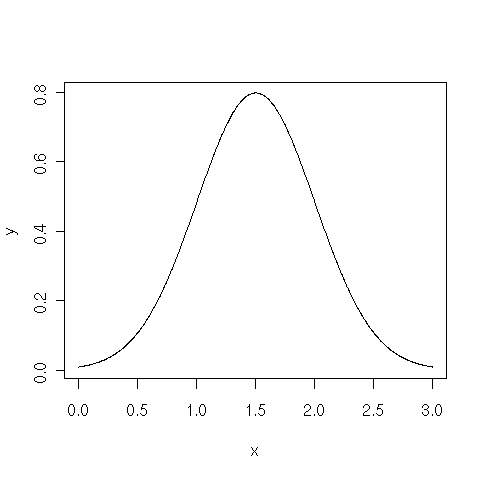
\includegraphics[scale=0.5]{chiron/normal.png}
	\end{center}
	\caption{normal}
	\label{fig:normal}
\end{figure}

\begin{figure}[h]
	\begin{center}
		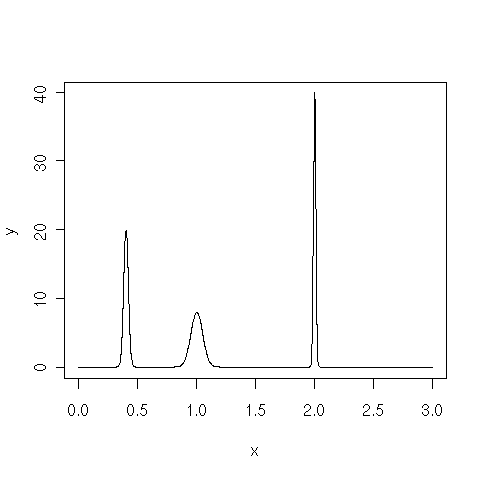
\includegraphics[scale=0.5]{chiron/pics.png}
	\end{center}
	\caption{Suma de Gaussianes difícil de trobar per Chiron} 
	\label{fig:dificil}
\end{figure} 

La solució que s'ha adoptat ha estat la de generar una població d'individus
nova, sense tenir en compte ĺa generació anterior, com si es comencés un
experiment nou.  Fent això evitem que l'algoritme genètic estigui ``viciat'' de
bon principi, i maximitzem les probabilitats de trobar algun pou d'energia
(\ref{ssub:CInicialitzacio}).

Les proves de correctesa del programa, s'han fet amb funcions matemàtiques
contínues, per tal de saber del cert que l'algorisme funciona bé i més endavant
s'ha provat amb el cas real de química combinatòria.

%Els resultats obtinguts d'aquestes funcions també seran exposats més endevant
%en l'apartat de resultats. 

\subsubsection{Testeig} % (fold)
\label{ssub:Testeig}

Hi ha un conjunt de funcions matemàtiques que es consideren ``típiques'' per a
usar-les com a ``problemes joguina'' (toy problems), per exemple, s'ha provat
l'algoritme evolutiu representant una funció on cada al·lel només té dos
possibles valors , 0 i 1, i la funció únicament suma els bits dels cromosomes.
El que es busca en aquesta funció, és maximitzar o bé minimitzar el resultat de
la suma de bits.  Aquest, tot i ser un exemple trivial, ens serveix per
saber si l'algorisme evolutiu funciona correctament.  Aquest exemple també ens
serveix perquè les mutacions i creuaments utilitzats són els mateixos que
utilitzem en la versió final de la aplicació.

Els resultats obtinguts són bons, arribant al millor resultat (tot uns) o a un
dels millors explorant només un percentatge de aproximadament el  10\% de
l'espai de cerca.

La funció de la suma de bits és una funció trivial per a qualsevol algorisme
evolutiu, donada la seva simplicitat.  És per això que després de provar amb
aquesta funció, hem provat funcions més complicades d'optimitzar, fins a arribar a
les conegudes com a ``funcions trampa''(\ref{EU2009}).  Les funcions trampa són funcions que
tenen característiques que fan molt difícil als AE trobar el màxim/mínim global,
tenint el millor resultat global envoltat de resultats molt dolents, i tenint un
màxim/mínim local ``fàcil'' d'arribar-hi en un extrem, apartant les solucions de
l'òptim global.  Una de les funcions trampa que hem provat, és la de mapejar en
un vector de bits una valoració determinada per a cada suma de bits.  Per
exemple, donat un vector de 5 posicions:

 % theme=Berlin;caption_top=1;caption=Exemple tanimotos
 % bits a 1 & valor
 % 0 & 1
 % 1 & 2
 % 2 & 3
 % 3 & 4
 % 4 & 5
 % 5 & 0

\begin{table}
\centering
\caption{Funció trampa}
\begin{tabular}{|r|r|}
\hline
\multicolumn{1}{|c|}{\textbf{bits a 1 }} & \multicolumn{1}{c|}{\textbf{ valor}} \\
\hline
\hline
0 & 1 \\
1 & 2 \\
2 & 3 \\
3 & 4 \\
4 & 5 \\
5 & 0 \\
\hline
\end{tabular}
\end{table}


L'ideal en aquest cas és trobar el vector que té 5 bits a 1, és a dir, busquem
minimitzar la funció.  Això, clarament és una trampa per a l'algorisme genètic,
ja que al fer els creuaments entre dos cromosomes que tenen una bona puntuació,
fa que els resultants, siguin molt dolents. És una manera d'enganyar al
algoritme evolutiu que ens serveix per a saber si aquest és prou robust per a
trobar un resultat bo.  En aquests casos, l'elitisme, és molt determinant per a
obtenir bons resultats.
% subsubsection Testeig (end)

%SOAP
\subsubsection{Funció fitness configurable} % (fold)
\label{ssub:Funcio fitness configurable}

Un altre aspecte important de Chiron és la versatilitat que té per a executar-se
amb diferents funcions de fitness.  Com s'ha explicat en la introducció del
capítol, Chiron permet avaluar manualment cadascun dels elements.  Donat que una
avaluació d'una molècula pot portar dies o setmanes, l'algorisme genètic ha de ser
capaç de mantenir l'estat i congelar-se a cada iteració.

Les llibreries usades (eodev), estan preparades per a mantenir l'estat en arxius
de text pla, però ho fan en el moment que s'ha acabat de executar la funció
avaluació de tots els individus d'una generació.  Per a poder aturar la
execució abans (a nivell lògic), el que hem dissenyat és un sistema per a
recollir i posar dades automàticament en els arxius de estat.  eodev està
programat en c++, i per tant, la funció de fitness ha de ser sempre la mateixa
ja que només volem tenir una instància de \texttt{Chiron} per executar, i no pas
una per a cada projecte que es faci.  El que hem fet per a solucionar aquesta
qüestió és ``anul·lar'' la funció de fitness fent que sigui una stub, que dona
fitness zero a tots els individus que avalua.  Configurant Chiron per a què
faci una sola generació, aconseguim guardar l'estat en un arxiu, amb els
paràmetres del algorisme genètic, les llavors (seed), i els individus de la
generació actual.  Llavors, el programa que executa el nucli de Chiron pot
parsejar l'arxiu, i insertar els elements en una base de dades (ens interessa
tenir un històric de tots els elements avaluats en generacions prèvies).
Aquests resultats són els que es presenten al usuari, que pot recuperar quan
vulgui ja que la recuperació de les dades es fa des de la base de dades MySql.

Quan l'usuari disposa de dades sobre les molècules, les pot introduir a través
d'una interfície, i tornar a executar una generació.

Si l'usuari ha configurat el projecte perquè mantingui els valors d'avaluacions
passades, en el moment que Chiron detecta una molècula que ja ha estat avaluada,
no li presenta al usuari, i és Chiron qui s'encarregarà de afegir el resultat en
el moment de la següent generació.

%subsub?  PRoblemes d'inicialització.

En  molts casos reals, ens trobem que tenim una immensa majoria de valors iguals
com a resultat de les avaluacions.  Aquests resultats són per les molècules que
o bé no poden ser sintetitzades, o bé no superen un llindar mínim d'activitat.
La manera com hem solucionat aquest problema s'explica detalladament en
l'apartat \ref{ssub:CInicialitzacio}.

% subsubsection Funció fitness configurable (end)

%BBDD
\subsubsection{Emmagatzematge de les dades} % (fold)
\label{ssub:Emmagatzematge de les dades}

Per a guardar l'estat del procés, hem creat una base de dades que ens permet
accedir i modificar la informació de un projecte.  La implementació d'aquesta
base de dades la hem fet amb MySql (més endavant es discutirà el perquè de la
elecció d'aquesta tecnologia en front a altres bases de dades, o altres
tècniques per a emmagatzemar dades (com poden ser Tokyo Cabinet/Tyrant, MongoDB
o altres SGBDs orientats a Documents,o diccionaris clau-valor).

\lstset{language=sql, tabsize=2}
\lstset{commentstyle=\textit}
\lstinputlisting[frame=trbl]{chirondb.sql}

Aquesta estructura ens permet tenir un historial de tots els elements que han
anat construint-se en els diferents experiments per a futurs anàlisis i
visualitzacions.
% subsubsection Emmagatematge de les dades (end)

\subsubsection{Webservice d'algorismes genètics} % (fold)
\label{ssub:Webservice d'algorismes genetics}

%SaaS WEB i SOAP
Una vegada tenim desacoblats el nucli (algoritme evolutiu), de la base de dades,
i del wrapper que va executant el nucli sobre els diferents projectes, i gestiona
la base de dades, ja tenim un programa funcional, que ens permet fer el que
volem.  Però encara tenim l'impediment de la interfície.  Un programa amb
múltiples usuaris, pensat per a solucionar problemes molt diferents entre si
(sempre pensant amb la química combinatòria com a funcionalitat principal,
 però intentant generalitzar i aconseguir la màxima abstracció possible), hauria
de tenir una interfície que permeti la execució del programa des de punts
diferents de un procés i des de diferents interfícies (front-ends).

Pensant amb la química combinatòria, la aplicació s'ha pensat des
d'un principi amb una interfície web en ment.  Per això, com a objectiu
principal, la interfície que fem a Chiron ha de permetre l'accés web.  Una
interfície web permet al usuari connectar-se des de on vulgui, sempre i quan
tingui accés a la xarxa, i un usuari habilitat.  Un avantatge clar de les
interfícies web és que l'usuari no haurà d'instal·lar cap programari per a executar
Chiron.  Per als interessos comercials d'Intelligent Pharma, també ha estat un
punt important, ja que l'usuari  final (client), pot rebre actualitzacions i
millores sense haver de fer res en absolut, sinó que tot el control recau sobre
el distribuïdor del programa.

Altres avantatges d'utilitzar un model de negoci ``Software as a Service''
(SaaS) és que el control del software recau sobre el distribuïdor, no només en
termes de actualitzacions i seguretat, sinó que obre noves possibilitats en
termes de models de pagament.   Per exemple, al no distribuir un software,
s'elimina la possibilitat de violacions de contracte o còpies il·legals, ja que
l'usuari no disposa mai del software, fent impossible la còpia, o l'ús
fraudulent d'aquest.  Les estadístiques que pot treure el distribuïdor (complint
els contractes de privacitat, és clar), son molt més potents que els clàssics
``bug reports'', podent acurar molt més el producte a les necessitats dels
usuaris, ja que sabent quines funcionalitats utilitzen més, o bé quins workflows
segueixen, podem tenir indicis de què i com s'ha de millorar.

Aquesta tendència del SaaS, està essent molt utilitzada en els darrers anys en
front al clàssic software instal·lat al client ja que, amb l'augment d'importància
del Cloud computing, i les tecnologies distribuïdes (Grid, globus, web 2.0), la
idea és que l'usuari d'un producte, sigui únicament això, un usuari d'un servei,
però no hagi de tenir cap coneixement ni infrastructura prèvia per a
utilitzar-lo.

SaaS també ha despertat dubtes i queixes, bàsicament en dues vessants:

Una d'elles és la dependència en el proveïdor de software.  No tenir cap tipus
d'infrastructura, suposa estar en mans del proveïdor, i per tant, si els
servidors del proveïdor no funcionen bé, o hi ha problemes d'accés, l'usuari
no controla les dades, ni pot fer res més que posar-se en contacte amb el
proveïdor del servei.  Aquesta falta d'autosuficiència fa que encara generi
desconfiança en certs sectors.

La privacitat també és un altre punt on s'ha generat certa desconfiança.  Les
dades, tot i que són accessibles per l'usuari, estan emmagatzemades en els
servidors del proveïdor.  Tot i que la legislació és molt clara al respecte,
hi ha clients que desconfien.

%WEB
Per altra banda, el testeig i la automatització de procediments a través de la
web és difícil per definició (no té estat, i les maneres més ``sofisticades''
per interactuar amb elles són macros no gaire intel·ligents).

Si només proporcionéssim interfície web, Chiron estaria sempre supeditat a la
utilització interactiva amb un usuari a l'altra banda.  Tot i que per Chiron, ja
serviria, hem de pensar en línies de futures aplicacions.  És per això que la
web no es comunica amb Chiron directament, sinó que hem programat una interfície
per a execució remota, i la web es comunica amb la interfície intermitja.

Aquesta interfície intermitja ens dóna la funcionalitat de poder accedir al
nucli de Chiron a través de programes, convertint Chiron en un servidor 
d'algoritmes genètics.

%Client-servidor. explicar una mica de que va el paradigma
Per a implementar el servidor de aplicacions remotes, s'han estudiat diverses
opcions, i ens hem decantat per a implementar una interfície SOAP.  Tot seguit
es discutiran les diferents opcions, i el perquè de la elecció, i en l'apartat
de implementació, es detallarà més la implementació de SOAP, i el funcionament
intern d'aquest.

%Execució remota
%RMI
%CORBA
%REST
%XML-RPC
%SOAP

Per a convertir Chiron en un servidor de algorismes genètics, que sigui usable
tant per persones (a traves de la web) com per aplicacions que connectin una
funció de fitness definida per elles al algorisme genètic, hem estudiat diverses
opcions, que analitzarem per sobre (donant algunes referències bàsiques).

L'objectiu és trobar una tecnologia que permeti fer crides remotes a un servidor
de funcions.  Com que el control del estat del programa el tractem manualment
(base de dades, etc) no necessitem que el sistema ens guardi la persistència.
Si utilitzéssim un sistema així també tindríem problemes a la hora de aturar el
servidor, i hauríem de crear un sistema de backups, amb lo que no ens
estalviaria la feina.

Necessitem doncs, exposar al exterior un conjunt de funcions aïllades, seguint el
paradigma client-servidor, que siguin extensibles i interpolables entre
diferents llenguatges de programació. Es pot veure la estructura de la
comunicació entre els processos en la figura \ref{fig:401px-Orb.png}.

\begin{figure}[h]
\centering
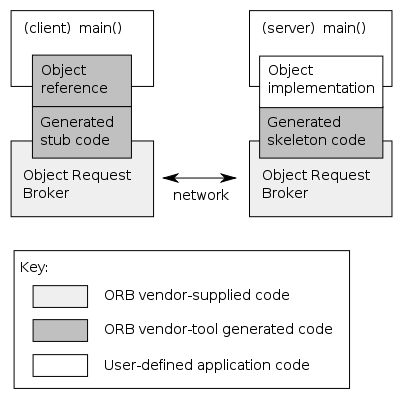
\includegraphics[scale=0.5]{401px-Orb.png}
\caption{Model de Client-servidor que necesitem}
\label{fig:401px-Orb.png}
\end{figure} 

Tecnologíes per a executar RPCs (Remote procedure call) n'hi ha moltes
diferents. Les tecnologies que ens obliguen a utilitzar el mateix llenguatge de
programació han quedat descartades de bon principi, ja que un dels objectius
principals és precisament obrir el programa a futures aplicacions que puguem
crear.  És per això que RMI, que ens lliga a java no pot ser utilitzada.  

Una altra alternativa que hem estudiat és CORBA, que és un sistema molt extès
per a tipus d'aplicacions client-servidor en xarxa, i proporciona una capa
intermitja molt còmoda i extensible.  CORBA és un sistema dissenyat per a
comunicar diferents llenguatges entre si.  Per aquesta part, ens serveix per als
nostres requeriments, però el protocol de CORBA funciona utilitzant ports TCP
no estàndards, i fa que no puguem garantir la connectivitat si el client o bé el
servidor estan darrere d'un tallafocs (firewall).

La aplicació Chiron ha de funcionar a través d'una interfície web que estarà
allotjada en un servidor local, i nosaltres controlem la xarxa, però com que
part de la essència de Chiron és el sistema de algorismes genètics genèric, no
volem limitar-nos a la utilització únicament per web.  Per això, s'han seguit
buscant alternatives.

Per assegurar que no tenim bloquejos en la xarxa, hi ha sistemes dissenyats per a
treballar només a través de ports coneguts, i normalment oberts en qualsevol
xarxa amb connexió a internet.  Exemples d'aquestes tecnologies son XML-RPC, REST
i SOAP.
% subsubsection Webservice d'Algorismes genètics (end)

\subsubsection{Disseny global} % (fold)
\label{ssub:Diseny global}

Després de diverses iteracions sobre el disseny, la estructura global que ha
quedat del projecte \texttt{Chiron} és la mostrada en la Figura \ref{fig:disenyChiron}.

Chiron es pot integrar en altres programes ja existents de l'empresa, donant
suport amb els algoritmes evolutius.  
%(XXX: El diagrama s'ha de fer més específic per a Chiron).

\begin{figure}[h]
	\begin{center}
		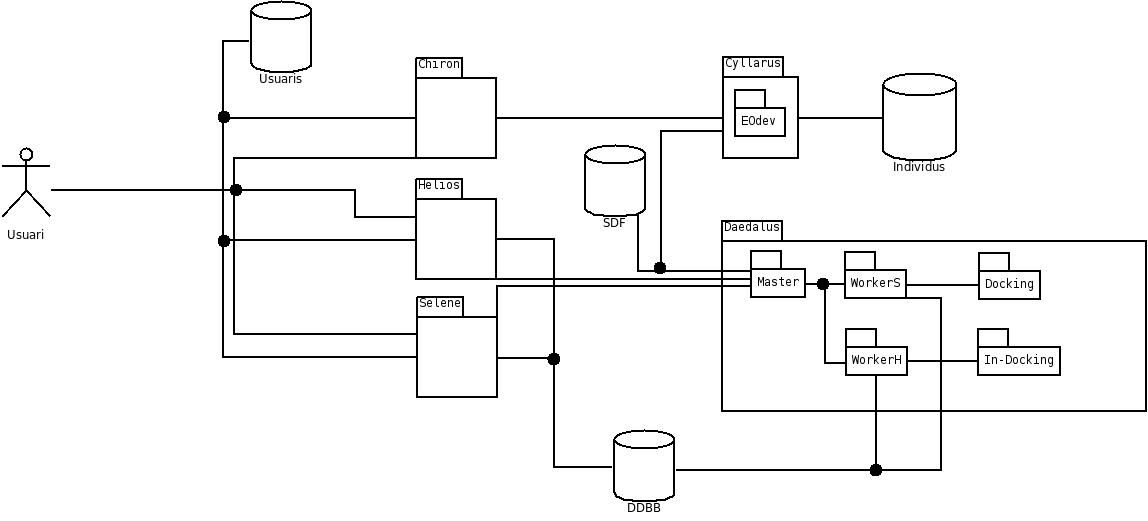
\includegraphics[scale=0.4]{chiron/arquitectura_global_chiron.jpg}
	\end{center}
	\caption{Es}
	\label{fig:disenyChiron}
\end{figure}
% subsubsection Diseny global (end)

% subsection Funcionament General (end)

\subsection{Algoritme Genètic} % (fold)
	\label{sub:Algoritme Genetic}
% subsection Algoritme Genetic (end)

L'algorisme genètic de Chiron, és un algorisme a ``mig implementar'', en el
sentit que  al ser parametritzable en quant a la funció de fitness, li falta una
de les parts principals dels algorismes genètics.  Això no vol dir que no haguem
implementat la funció de fitness, sinó queda externalitzada respecte el nucli de
\texttt{Chiron}.  Tot seguit s'explica la implementació de cadascun dels
paràmetres i estructures de dades necessàries per a la implementació de Chiron.

\subsubsection{Inicialització} % (fold)
\label{ssub:CInicialitzacio}

En  molts casos reals, ens trobem que tenim una immensa majoria de valors iguals
com a resultat de les avaluacions.  Aquests resultats són per les molècules que
o bé no poden ser sintetitzades, o bé no superen un llindar mínim d'activitat.

Això ens ha suposat un gran problema perquè si avaluem la primera generació i
tots els elements tenen el mateix fitness (0), la següent població que Chiron
suggerirà serà una població tal que haurà sortit de creuar i mutar la primera
població aleatòriament entre ella.  Aquest procediment ens provoca una
convergència prematura que no desitgem, ja que el que passa en realitat és que
encara no hem mostrejat cap molècula que ens doni un mínim d'activitat amb el
que poder ``jugar''.

Problemes d'aquestes característiques només es donen en casos on l'espai de
cerca és molt gran comparat amb el número de elements que tenen resultats
diferents de 0.

Per exemple, si volguéssim trobar, en el problema de la suma de bits una
configuració concreta (10101), o bé trobar elements amb unes certes
característiques (que sumin 3), i tots els elements que ho compleixen tenen
fitness 1 i els que no, tenen fitness 0, ens trobaríem amb problemes similars.

Aquest problema, l'hem solucionat provocant que Chiron resetegi l'experiment
(recordant les molècules avaluades en la base de dades), i torni a donar una
població d'individus aleatòria.  Així maximitzem les probabilitats de trobar un
o més pous energètics, que son les àrees del espai de búsqueda (normalment
contínues) on es troben els elements amb fitness superiors al llindar.  En el
moment que trobem molècules amb activitat, l'algorisme segueix el procediment
normal.

% subsubsection Inicialització (end)

\subsubsection{Individu (Cromosoma)}
\label{ssub:individu (cromosoma)}

En aquest algorisme genètic, els indicis són les diferents combinacions de
ramificacions, en cadascuna de les posicions. Com que els canvis entre un al·lel i un
altre són qualitatius, cada posició del cromosoma és un enter, que representa
una terminació diferent en funció de la posició on es troba dins el cromosoma.

Així doncs, tenim un vector de N posicions on N és el número de ramificacions que té
l'esquelet, i cada posició conté un enter, amb límits d'acord amb les
especificacions del usuari al iniciar el projecte. 

Utilitzem enters per a representar cada al·lel perquè és la forma més còmoda que
tenim per representar valors qualitatius o categòrics.  A més, els valors límit
de cada posició s'acoten en cada projecte.  Això és un altre tret que el
diferència de programes més estàtics on els límits són coneguts a priori, com
per exemple Pholus (\ref{cha:Pholus}).

Si els possibles valors adoptats en cada punt fossin coneguts en temps de
desenvolupament del projecte, es podria usar tipus enumerats, per a deixar ben
clar que els valors són qualitatius i que hi ha la mateixa diferència en un
al·lel entre el valor 1 i el 2 que entre el 1 i el 5, ja que simplement són
ramificacions diferents, i no tenen res a veure un amb l'altre.  Això també ens
condiciona els creuaments, com s'explica en la següent secció.

%PUNT

\subsubsection{Selecció} % (fold)
\label{ssub:CSeleccio}
En aquest problema, hem utilitzat un algorisme de sel·lecció per Torneig
determinista ($p=1$), on competeixen dos individus.  Donat que les poblacions
són relativament petites en la majoria de casos (tenim un espai total de cerca
de gairebé 16000), hem utilitzat un torneig petit, ja que la pressió evolutiva
que implica pujar el torneig en un és molt gran, i de seguida ens estanca en
problemes de convergència prematura.

% subsubsection Selecció (end)

\subsubsection{Creuament} % (fold)
\label{ssub:Crossover}

Com a operador de creuament entre 2 individus d'una generació, s'utilitza el
tall per 1 punt.  La raó d'això és que cadascun dels al·lels té un valor
qualitatiu, i no té cap sentit fer altres creuaments on el mateix gen (mateixa
posició del vector) es creua físicament amb el gen de l'altre cromosoma.

Un creuament que involucrés aritmètica no es pot fer servir en aquest cas ja que
no es poden sumar ``peres i pomes''.

Creuaments que involucrin el canvi de posició en els gens tampoc eren naturals
per aquest problema, ja que s'hauria de comprovar que cap gen es col·loca en una
posició on no pot ser-hi ja que supera els límits estipulats per la
posició final.  A part d'aquest fet totalment subjecte a implementació, i per
tant, solucionable amb una mica més de comprovacions, aquests creuaments no
tenen sentit químic, ja que l'alternativa $i$ de la posició $n$, no té perquè
tenir res a veure, ni cap correlació amb l'alternativa $i$ de la posició $m$ on
$n <> m$.

Pel creuament s'ha provat un creuament per un punt, i el creuament per dos
punts, donant resultats similars en els dos casos.  Donat que els experiments
químics en què s'ha provat (\ref{sec:Resultats}), tenen només tres llocs per a
substituents, un creuament per diversos punts no tenia gaire sentit.

Donats dos individus (els que han estat sel·leccionats en el procés de
sel·lecció per a reproduir-se , amb una probabilitat d'un 0.8 es fa creuament i
els fills són tan sols una partició formada a partir dels 2 pares, amb un punt
de tall aleatori.  Donat que no hi ha cap relació entre els diferents indexos
(estan ordenats arbitràriament) no ens hem de preocupar de partir el cromosoma
per lloc ``delicat''. 

Així doncs, el que es busca és interpolar les qualitats de dos individus ben
adaptats, per a crear uns descendents amb propietats similars.  És d'esperar que
si un individu té bon fitness, les ponderacions donades als seus indicadors
siguin bastant encertades.  Llavors, en interpolar una parella de individus,
suposem que el descendent també tindrà un fitness bo, i això farà que a mesura
que passen les generacions, la població tendeixi a millorar (en mitja).

En els experiments en formules matemàtiques, ha donat millors resultats el tall
en 2 punts, que no pas en 1.

% subsubsection crossover (end)

\subsubsection{Mutacions} % (fold)
\label{ssub:Mutacions}

La única mutació que té sentit en aquest problema és canviar un dels elements
del cromosoma per un altre, sempre dins del rang que tingui en aquesta posició.

Intercanvis de al·lels de diferents posicions no són possibles ja que les
diferents posicions del cromosoma tenen rangs diferents, i fa que molts dels
intercanvis que faríem siguin invàlids.
% subsubsection Mutacions (end)


\subsection{Implementació} % (fold)
	\label{sub:Implementacio}

Tot seguit es detallen algunes particularitats de la implementació de
\texttt{Chiron}, amb les seves tecnologies, i algun codi exemplificador del que
s'està explicant.

\subsubsection{Algorisme genètic} % (fold)
\label{ssub:algorisme genetic}

En aquest projecte s'han utilitzat les llibreries eodev, igual que en el
projecte \texttt{Pholus}, ja que ens proporcionen les qualitats suficients per a
poder treballar per sobre d'elles sense haver de fer gaires modificacions sobre
el seu codi base.

Eodev proporciona una estructura genèrica per a algorismes genètics, on, si no
volem massa complicacions, amb un cromosoma de coma flotants, modificant només
la funció de fitness, podem corre ja el nostre algorisme genètic.  Això no ens
serveix per a \texttt{Chiron}, ja que necessitem modificar el cromosoma, les
mutacions i creuaments per al que volem fer nosaltres.

Hem de crear doncs, una classe per a cada element del algorisme genètic.

%PUNT posar totes les classes

% subsubsection algorisme genètic (end)

\subsubsection{Arxius de configuració} % (fold)
\label{ssub:Arxius de configuracio}

Eodev disposa d'una manera per llançar execucions amb un arxiu de configuració
determinat.  El format no respon a cap estàndard (ni .ini, ni .conf\ldots).
Aquest format és el que fem servir per a llançar procéssos \texttt{Chiron}, amb
els parametres adequats, i per altra banda, entre generació i generació, omplim
els fitness en l'arxiu aquest.  És una manera de colar-se en el procediment de
Chiron, i permetent-nos modificar el fitness d'un element en una generació
determinada.

Per a generar aquest arxiu de configuració hem agafat un dels de demostració que
vénen amb les fonts de Eodev, i hem creat un template o plantilla, utilitzant
Template Toolkit (TT\footnote{\url{http://template-toolkit.org/}}).
\cite{CCW03}.

Template Toolkit és una llibreria molt estesa per a la generació de textos
parametritzats.  En un principi es va crear per a reproduir textos massivament,
on només canvia una petita part del text (per exemple, circulars), o bé arxius
que han de complir una certa estructura (webs corporatives).

Nostres hem usat la implementació en Perl, que a part de ser la primera que va
sortir (i potser la més sòlida), és el llenguatge en el que hem desenvolupat
tota la part que no forma part del nucli de la aplicació.  Segueix un exemple de
la utilització de Template Toolkit en un cas senzill, i la manera en que ens
facilita la separació de la presentació de la lògica.  És per això que Template
Toolkit també s'utilitza en molts frameworks web perl\footnote{Catalyst.
http://www.catalystframework.org/}.

%codi Template Toolkit
\lstset{language=perl, tabsize=2}
\lstset{commentstyle=\textit}
\lstinputlisting[frame=trbl]{tt.pl}

Encara que en aquest exemple, no sembla més que una versió ``més elegant'' de
sprintf, Template Toolkit pot afegir lògica en les seves plantilles, processant
o no processant arxius en subdirectoris, en funció de valors de variables en el
programa perl que crida les funcions TT.

% subsubsection Arxius de configuració (end)

\subsubsection{DBIx::Class} % (fold)
\label{ssub:DBIx Class}

Tant l'arxiu de configuració de cada projecte, com la informació dels individus
que han aparegut en generacions passades del projecte, i com el propietari de
cada projecte es mantenen en una base de dades MySql.

La decisió de MySql o bé PosgreSql, no ha estat una decisió on hi hagi hagut un
clar guanyador.  Pel volum de dades que hem de tenir, tampoc creiem que això
sigui una decisió critica per al èxit del projecte, però per si de cas, hem
decidit utilitzar un sistema de ORM \footnote{Object Relational Mapper} .

Els ORMs són llibreries que mapegen taules SQL a objectes del llenguatge, podent
així fer més directe el tractament amb bases de dades des de llenguatges de
programació, fent que no s'hagi de fer un canvi de paradigma tant gran al
canviar de OOP pura a \texttt{SELECT * FROM \ldots}.

Sabem doncs, que per al projecte, en l'estat actual no és necessari plantejar-se
quina és la millor base de dades a escollir, si hem fet una bona elecció pel
que fa a les eines i llibreries, ja que utilitzant DBIx::Class, canviar de SGBD no
suposa cap modificació en el codi, fent-ho del tot transparent.

% subsubsection DBIx\dots Class (end)

\subsubsection{Webservices i Soap} % (fold)
\label{ssub:WS i Soap}

Com ja s'ha explicat anteriorment (\ref{sec:Procediment informatic} ), per a la
comunicació segons el paradigma client-servidor, s'ha utilitzat la tecnologia
SOAP\footnote{Simple Object Access Protocol}.

Els seus rivals més igualats, per als nostres requeriments, han estat XML-RPC i
REST, però hem decidit utilitzar SOAP, entre d'altres coses, perquè és l'únic
que té suport a nivell corporatiu, i no com REST, que son estàndards
desenvolupats majoritàriament en entorns de comunitats Opensource.  Al
utilitzar-lo nosaltres en un entorn corporatiu, hem pensat que SOAP seria més
adequat pel possible suport que tindria i la interpolabilitat amb altres
aplicacions que es poden utilitzar en el futur.
%PUNT . POSAR L'ESTANDARD SOAP, I WSDLs i XMLs d'exemple?

% subsubsection Webservices i Soap(end)
% subsection Implementació (end)
% section Procediment informàtic (end)

\section{Resultats} % (fold)
	\label{sec:Resultats}

	En les proves que hem realitzat, \texttt{Chiron} ha donat bons resultats,
	però necessitem fer algunes validacions per a assegurar que ha valgut la
	pena aquest esforç, i també tenir dades objectives sobre la seva utilitat.
	A nivell comercial, també es vol tenir alguna validació estadística que ens
	doni seguretat per a ``vendre'' Chiron.

	Per a realitzar les proves inicials, s'han utilitzat funcions típiques de
	testeig d'algorismes genètics, com la suma de bits (es tracta de maximitzar
	el número de bits a 1 en un vector), o alguna funció trampa, on el màxim de
	la funció no està en cap extrem del espai de búsqueda.

	Les proves sobre un escenari real en el que operarà Chiron, s'han fet sobre
	tres projectes dels quals s'ha realitzat la prova experimental de totes les
	combinacions de substituents possibles (s'han trobat en (XXX Ppaper) )

	En aquests tres problemes, els autors dels experiments van sintetitzar totes
	les possibles molècules, obtenint un resultat de activitat en cadascuna
	d'elles.  És possible que algunes d'elles fossin impossibles de sintetitzar,
	i que els hi haguessin posat un fitness molt baix.  Això ja ens va bé per
	als nostres propòsits, ja que és el mateix resultat que els hi donaríem
	nosaltres.

	Per a testejar Chiron, hem usat un programa de test, que analitza totes les
	dades experimentals, tenint així una resposta per a cada possible individuu
	que pugui proposar Chiron.

	Aquest programa de prova, ha estat desenvolupat en Perl, atacant directament
	la llibreria també programada en perl, no pas usant la interfície SOAP, ja
	que podent fer les proves en local, és molt més ràpid en executar-se.

	S'han fet 25 execucions de Chiron per a cada projecte, i hem
	esperat a què convergeixin cadascun dels 3 projectes.  Com que tenim a la
	nostra disposició totes les dades del espai de cerca, hem fet càlculs
	respecte quantes avaluacions s'han fet fins a trobar el millor element que
	hem arribat a trobar.  També ens fa falta saber quin és el fitness d'aquest
	element, i quin és el fitness de la millor combinació de substituents que
	hi ha en tot l'espai de cerca. 

	%TAULA de resultats.

% theme=Berlin;caption_top=1;caption=Exemple tanimotos
% BBDD & Fitness & Elements avaluats & relació

%png('file.png')
%hist(x)
%dev.off()

	En les figures \ref{fig:resChir1},\ref{fig:resChir2} i \ref{fig:resChir2} es
	mostren les validacions que s'han fet a Chiron.  

	\begin{figure}[tbp]
		\begin{center}
			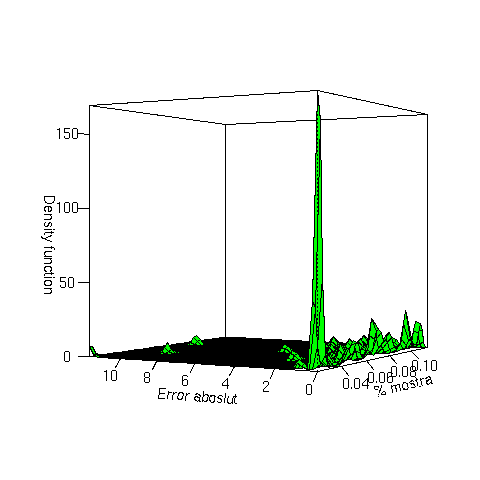
\includegraphics[scale=0.75]{chiron/rgrau1.png}
		\end{center}
		\caption{Resultat Chiron 1}
		\label{fig:resChir1}
	\end{figure}

	\begin{figure}[tbp]
		\begin{center}
			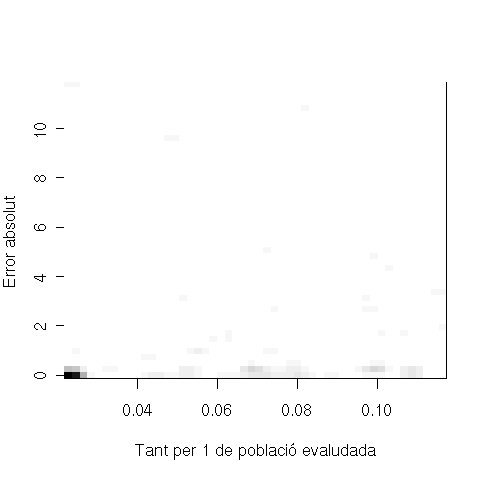
\includegraphics[scale=0.75]{chiron/GraficaChironGuai.png}
		\end{center}
		\caption{Resultat Chiron 2}
		\label{fig:resChir2}
	\end{figure}

	\begin{figure}[tbp]
		\begin{center}
			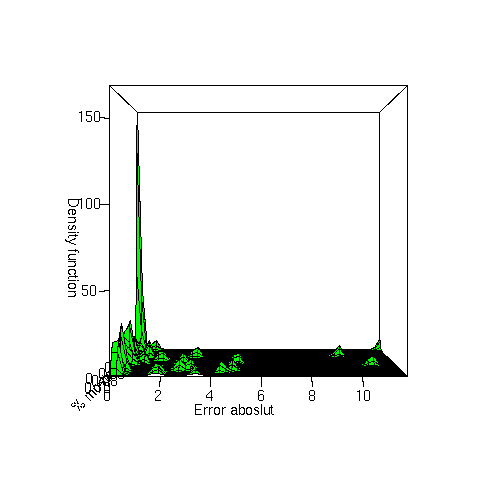
\includegraphics[scale=0.75]{chiron/rgrau3.png}
		\end{center}
		\caption{Resultat Chiron 3}
		\label{fig:resChir3}
	\end{figure}
	\begin{figure}[tbp]
		\begin{center}
			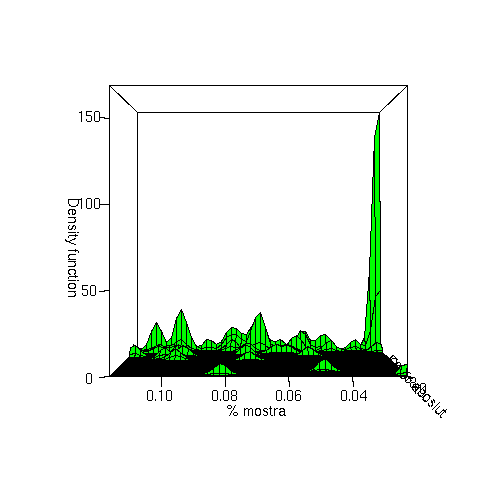
\includegraphics[scale=0.75]{chiron/rgrau4.png}
		\end{center}
		\caption{Resultat Chiron 3}
		\label{fig:resChir4}
	\end{figure}

	Aquestes gràfiques mostren, de diferents maneres, el nombre de elements
	avaluats, i l'error absolut que s'ha obtingut en cadascun dels experiments.

	La intenció inicial era utilitzar l'error relatiu, però en aquests
	experiments, els pitjors fitness tenen un valor de infinit.  Com que els
	tres experiments sobre els que hem fet les proves són molt similars en quant
	al millor fitness possible (0, 0.1 i 0.09), hem pogut dissenyar un
	sistema de tests unificant els resultats dels tres experiments, i així tenir
	una idea més general del rendiment de \texttt{Chiron}.

	Com ja s'ha dit prèviament, s'han  realitzat 25 execucions de cadascun dels
	tres experiments, guardant per a cadascun el número d'individus que s'han
	avaluat, el número total d'individus del espai de cerca, el millor fitness
	de tot l'espai de cerca, i el millor fitness al que hem arribat.

	D'aquesta manera, hem pogut fer un estudi estadístic sobre el funcionament i
	rendiment de Chiron.

	L'estudi, estadístic, l'hem realitzat utilitzant el software estadístic
	R(\url{http://www.r-project.org/}), i ens permet dir coses com per exemple, que \textbf{avaluant un XXX
	\% de l'espai de búsqueda, ens quedem a XXX del millor en un XXX dels casos}


\section{Conclusions i treball futur} % (fold)
\label{sec:CConclusions i treball futur}

	Amb tot el desenvolupament i proves realitzades, hem assolit l'objectiu
	d'aquesta part del PFC.  Tot i això com a projecte futur
	d'ampliació, està implementar tècniques de algorismes genètics interactius.

	Donat que la avaluació és supervisada per l'usuari, podríem implementar
	tècniques per a classificar els individus de cadascuna de les generacions,
	per a només donar al usuari una part de la població a avaluar, en funció de
	la semblança entre els individus.  Es podria utilitzar alguna tècnica de
	clustering, o eines més particulars d'algorismes genètics interactius.
	% subsection treball futur (end)
% section Resultats (end)

%\end{document}
%# vim: set tabstop=4 shiftwidth=4 tw=80 foldmethod=marker ignorecase : ##

% chapter Chiron (end)
\documentclass[titlepage,a4paper,12pt]{book}

\usepackage[utf8]{inputenc}
\usepackage[catalan]{babel}
\usepackage{graphicx}
\usepackage{verbatim}
\usepackage{marvosym}
\usepackage{amssymb, amsmath} 
\usepackage{listings}
\usepackage{textcomp}
\usepackage[]{color}

%\lstset{
	%language=C++,
	%keywordstyle=\bfseries\ttfamily\color[rgb]{0,0,1},
	%identifierstyle=\ttfamily,
	%commentstyle=\color[rgb]{0.133,0.545,0.133},
	%stringstyle=\ttfamily\color[rgb]{0.627,0.126,0.941},
	%showstringspaces=false,
	%basicstyle=\small,
	%numberstyle=\footnotesize,
	%numbers=left,
	%stepnumber=1,
	%numbersep=10pt,
	%tabsize=2,
	%breaklines=true,
	%prebreak = \raisebox{0ex}[0ex][0ex]{\ensuremath{\hookleftarrow}},
	%breakatwhitespace=false,
	%aboveskip={1.5\baselineskip},
  %columns=fixed,
  %upquote=true,
  %extendedchars=true,
%% frame=single,
%% backgroundcolor=\color{lbcolor},
%}

\begin{document}
\tableofcontents  %%Index

\section{Introducció} % (fold) Objectius?
	\label{sec:Introduccio}
	Tot seguit es presentará un projecte en el que s'ha utilitzat una tècnica
	molt pionera derivada de la programació genètica anomenada ``Genetic
	Expression Programming'' (GEP).


% section Introducció (end)

\section{Context Químic} % (fold)
	\label{sec:Context Quimic}

\section{Procediment informàtic} % (fold)
\label{sec:Procediment informatic}

El diseny i implementació  d'aquest projecte és la que s'ha emportat més temps
proporcionalment, ja que s'ha hagut de fer molta investigació per a ajustar els
paràmetres del algorisme genètic, i per a implementar els diferents operadors.

Ens enfrontem a un problema on el cromosoma, a diferència Pholus i Chiron, no
pot ser tractat com un vector d'elements independents, ja que s'ha de mapejar un
arbre (que representa una fórmula analítica) en un vector, i un gen
\textit{i} té molta repercusió en els seus gens posteriors.

La manera clàssica d'atacar els problemes de programació genètica, és
confeccionant una representació d'un arbre en el cromosoma, en preordre,
inordre, o postordre.  Cadascuna d'aquestes implementacions suposa uns pros i
uns contres, ja sigui en la construcció, la interpretació (per a executar la
funció de fitness s'ha d'evaluar el resultat, i per tant, s'ha de reconstruir
l'arbre), o en els diferents operadors, tant el creuament com la mutació.

Com a primera aproximació, s'ha implementat un arbre en preodre, ja que facilita
molt la evaluació, una de les parts més costoses i que s'ha de fer més cops al
llarg del algoritme.

Imaginem que tenim un arbre de la següent manera:

\begin{verbatim}
+ 2 - 3 2
\end{verbatim}

Aquest arbre, que traduit a inordre és $ 2 + (3 -2) $ , pot ser calculat
construint un evaluador com una màquna de pila, on apilem els elements a mesura
que els anem trobant, i evaluem les operacions una vegada tenim els operands
suficients per a la última operació que hem apilat.

La construcció en preordre deixa les fulles al final dels subarbres, i això és
convenient en la mesura del possible, ja que per als creuaments, augmenta la
possibilitat de crear un arbre vàlid. % XXX REF a creuaments

Un dels problemes que es donen en els algorismes de programació genètica, és la
construcció d'arbres invàlids. Per exemple, suposem que fem un creuament per un
punt de tall entre dos arbres, com si fós un algorisme evolutiu clàssic.

\begin{verbatim}
+ 3 * 3 | - 4 3
- Q + * | 5 3 5
\end{verbatim}

al intercanviar els arbres, un dels 2 arbres que queden (- Q + * - 3 5) no
disposa de prous operands per a realitzar la evaluació.  Això és un cas senzill
de tots els problemes que es poden generar al fer creuaments, i és el cas en el
que utilitzem el creuament més trivial (creuament per un punt). Si utilitzéssim
creuaments més sofisticats, els casos que hem de tractar particularment per
creixen molt de pressa.  Només fent un creuament per 2 punts, es generen
moltíssims més arbres sintacticament incorrectes.

És per això que s'ha adoptat finalment per una aproximació utilitzant una
representació ideada per Ferreira (XXX bib), on per la pròpia construcció del
arbre, podem assegurar que \textbf{sempre} generarem arbres sintàcticament
vàlids.

\subsection{Interfície} % (fold)
\label{sub:Interficie}

L'usuari, en aquest cas encara no està molt definit, ja que segurament, GEP es
farà servir com a complement per a Helios 2.0, però les entrades al programa son
clares:

Es disposa de resultats empírics (o bé per laboratori o bé utilitzant softwares
de simulació) sobre, per exemple, el volum d'una molècula en funció dels angles
dels seus enllaços rotables.

En un cas així, les dades d'entrada són els diferents angles i els volums
obtinguts, i el que es demana a la aplicació, és que a partir d'aquestes dades,
trobi una fórmula analítica que representi (amb la major fiabilitat possible)
aquestes dades, per a poder generalitzar les dades empíriques a una fórmula
tractable matemàticament.

El programa ha d'executar-se d'una tirada, amb el que no tindrà cap component de
interactivitat, ni es necessitarà cap tipus de emmagatzematge de dades
intermitges.

La entrada, doncs, es fa a través d'un paràmetre que ens indica on estan els
resultats que coneixem, juntament amb les dades que ens porten a aquests.

Juntament amb les dades, també s'han d'entrar els diferents paràmetres referents
al algorisme genètic.  Ara per ara no està implementat, però com es veurà en
l'apartat de treballs futurs(XXX), s'ha pensat permetre a l'usuari (se'l
considera un usuari ``expert'', que coneix tant el problema, com té coneixements
d'algorismes genètics) entrar ``building blocks'' addicionals, o
activar/desactivar els que ja venen per defecte.

Això suposa un gran repte a causa de les característiques estàtiques del
llenguatge, però ja s'han estudiat algunes maneres per a poder utilitzar
tècniques que permeten ``dinamitzar'' el llenguatge (utilitzant plugins o
llenguatges de scripting acoblats (embeded) al programa c++.
% subsection Interficie (end)


\subsection{Preparació de les dades} % (fold)
\label{sub:GPreparacio de dades}

La preparació de dades necessària per a aquest projecte no té massa rellevància,
ja que disposem a priori dels conjunts de dades d'entrada i resultats.

El programa simplement agafa les dades d'uns arxius que hem tractat amb uns
petits scripts per a tenir un format realment còmode.

Per a les proves que s'han realitzat per descubrir funcions matemàtiques
conegudes, la mateixa funció s'ha implementat en la funció d'evaluació, i
simplement, s'executa amb les dades d'entrada, per a tenir el resultat a
comparar-lo amb el resultat de la formula que estem evaluant.

% subsection Preparació de les dades (end)

\subsection{Implementació} % (fold)
\label{sub:GImplementacio}

Aquest projecte ha estat el més difícil d'implementar i disenyar, ja que hem
hagut de fer un treball notable d'investigació (els primers referents en GEP
daten de 2002 XXX).

El procés general del algoritme evolutiu és, donada una llargada de cromosoma,
decidida per l'usuari en funció de la complexitat ``intuitiva'' de la formula
que es vol descubrir, i uns paràmetres de probabilitat de creuaments i
mutacions, la aplicació ha de retornar una fórmula analítica que s'apropa (o
clava) la fórmula que estem buscant.
% subsection Impl (end)

(XXX) fer una seccio dedicada a GP i GEP o posar-ho a la implementació?

\subsubsection{Arbres} % (fold)
\label{ssub:Arbres}

Com s'ha explicat en \ref{introGEP i Procinf}, en GEP, la interpretació dels
cromosomes com a arbres a l'hora d'avaluar-se, fa que necessitem poder passar
del fenotip(lineal) al genotip (arbre) amb facilitat, i aquest genotip sigui
tractable com a tal, avaluant les seves característiques en l'entorn (calculant
l'arbre) de manera còmode, ràpida i eficient.

Per això s'ha desenvolupat un conjunt de classes per a tractar amb arbres, que
ens permeten construir i avaluar aquests arbres a partir d'un cromosoma (vector
de símbols).

Aquesta estructura, s'ha programat el més flexiblement possible, deixant la
possibilitat de ser extesa en un futur, afegint nous tipus d'operacions, i amb
diferents aritats, més grans de les que hem tingut necessitat fins al moment.

Nosaltres hem tractat només amb aritats 0,1 i dos (a € {0,1,2} ) ja que els
operands tenien un màxim de aritat 2.


 % theme=Berlin;caption_top=1;caption=Relació funció-aritat
 % simbol & aritat
 % + & 2
 % - & 2
 % * & 2
 % / & 2
 % sin & 1
 % cos & 1
 % sqrt (arrel quadrada) & 1
 % terminals (x,y,z..) & 0

\begin{table}
\centering
\caption{Relació funció-aritat}
\begin{tabular}{|l|r|}
\hline
\multicolumn{1}{|c|}{\textbf{simbol }} & \multicolumn{1}{c|}{\textbf{ aritat}} \\
\hline
\hline
+                     & 2 \\
-                     & 2 \\
*                     & 2 \\
/                     & 2 \\
sin                   & 1 \\
cos                   & 1 \\
sqrt (arrel quadrada) & 1 \\
terminals (x,y,z..)   & 0 \\
\hline
\end{tabular}
\end{table}

Per a poder construir un arbre complet, i avaluar-lo, a partir d'un vector de
simbols (implementats com a caràcters, donada la manca de símbols en c++ com a
tipus bàsic), i poder-ho fer amb la màxima robustesa i flexibilitat, s'ha
implemntat una estructura amb nodes, i un arbre tipus template.

Tot seguit es mostra el diagrama de classes d'aquesta part GEP.

%figura estructura de classes

Com es pot veure en la figura anterior (XXX ref fig), s'ha implementat una
classe abstracte Node de la que ``pengen'' les diferents especialitzacions, que
son les diferents operacions que suporta GEP, o bé els terminals. Els terminals,
com és d'esperar, tenen aritat zero, i al ser evaluats, retornen el valor del
terminal en aquest moment com a resultat.  Els operadors (aritat > 0),
requereixen d'altres nodes per a calcular el seu resultat.  D'això es deriva que
en un cromosoma donat, al transformarlo a genotip, les fulles seran totes
terminals, ja que son l'únic tipus de node que poden evaluar a un valor sense
necessitat de cap altre resultat precalculat.

Al haver-se de crear nodes dinàmicament (i intensament) durant cada execució,
s'ha utilitzat un patró \emph{Factory}, per facilitar la creació de nodes amb
una sintaxis extensible, per quan es vulguin afegir operadors, i per a fer més
còmode la seva utilització.

Després de implementar-se aquesta part, hem descobert una manera tant o més
elegant de fer-se aquest procés:  Utilitzant les llibreries Boost (XXX ref), que
ofereixen, entre d'altres, funcionalitatsl pròpies de llenguatges funcionals,
com per exemple Boost::Functional, que permet la programació de c++ retornant
funcions com a valor de retorn de una funció (programació d'ordre superior).  
D'aquesta manera, encara podem delegar un pas més avall la creació de nodes, 

arbres, nodes, evaluacio, etc.
patro estrategia + factory
Parlar de BOOST::Functional
% subsubsection Arbres (end)

\subsection{Algorisme Genètic} % (fold)
\label{ssec:GAlgorisme Genetic}

\subsubsection{Individu (Cromosoma)} % (fold)
\label{ssub:Individu (Cromosoma}

Per aquest s'han utilitzat els cromosomes representats com s'ha explicat en
l'apartat \ref{issub:individus}, però no només s'han utilitzat cromosomes amb un
gen, sinó que hem seguit dues altres maneres, més sofisticades per a representar
les nostres fórmules matemàtiques.

Aquests mètodes \cite (XXX) es basen en complicar una mica més el cromosoma,
però sempre fent servir la notacio karva \ref{XXX}.

Una de les millores, és encabir més d'un gen en un cromosoma. Fent això, el que
aconseguim és evolucionar dos subarbres, que en el moment de la avaluació,
s'uneixen d'alguna manera.

Si apliquem aquesta tècnica, es facilita la creació de subarbres que conformen
el que s'anomenen ``building blocks'', o blocks constructors que representen una
petita part (però significativa) de la fórmula que es vol acabar trobant.

EXEMPLE

Una de les maneres de combinar els diferents gens és utilitzant \emph{Link
functions} o funcions d'enllaç, que son operadors que decidim a priori, i
seràn els nodes arrel de l'arbre final.

En \ref{figXXX} es mostra com s'avaluarà el cromosoma mostrat abans amb funcions
d'enllaç suma.

Aquesta millora, dona molta flexibilitat al algorisme genètic, ja que li dona
poder per a fer combinacions entre diferents cromosomes (en el creuament), només
cambiant una part del arbre, i no fent cambis molt radicals al fenotip.  Aquest
procés de linkatge està també inspirat amb els procediments de la naturalesa per
a ensamblar proteïnes a partir de components més petites.

La següent implementació i millora és construir un gen una mica diferent en un
dels extrems del cromosoma, que contingui informació codificada sobre el propi
cromosoma.  Aquest tipus de metainformació és molt valuosa, i ens permet que el
propi cromosoma sàpiga com ensamblar-se i a més, ho pugui fer d'una manera
variable, que vagi evolucionant al mateix temps que evoluciona tot el propi gen.

El caire recursiu d'aquesta millora és una de les claus del bon funcionament de
GEP, ja que permet guardar una espècie d'``estat'', que ens dona dades sobre com
organitzar la pròpia informació que conté.

La manera de codificar-se, però, és molt similar a la que ja coneixem fins ara,
i gràcies a aquesta homogenietat, no s'han de fer tractaments especifics per a
aquesta metainformació ja que es codifica també amb forma d'un arbre amb notació
Karva, que en comptes d'utilitzar els terminals com a elements d'aritat zero, el
que s'utilitza com a elements ``de finalització'' són identificadors que es
refereixen als anteriors gens o ADT.

Com tots els gens, aquest gen especial, té un head i un tail, i en el seu head
es poden utilitzar els mateixos operadors que en la resta de heads.  Tot i així,
nosaltres hem reduit el nombre d'operadors a només $+,-,*,/$, descartant
operands com el sinus, cosinus i la arrel quadrada.

Com que el número de terminals diferents que pot tenir aquest meta-gen vé
determinat per el número total de gens amb els que configurem els cromosomes (el
número de terminals serà N-1 on N és el número total de gens), el número de gens
s'ha de saber al principi de la execució del programa, i no pot ser modificat
durant la execució (també violariem tota la homoiconicitat  d'un cromosoma respecte
els altres).

Per codificar aquests ``punters'' als ADTs, utilitzem números del 0..N-2
(seguint la mateixa notació anterior).

A continuació es mostra com un cromosoma multigènic homeòtic es codifica i
s'evalua.

% subsubsection Individu (Cromosoma (end)

\subsubsection{Inicialització} % (fold)
\label{ssub:Inicialitzacio}
La població inicial, inicialitza un número $N$ de cromosomes de manera
aleatòria.  La forma en què s'han d'inicialitzar els cromosomes és barrejant en
un mateix individu operadors i terminals, durant la ``zona de operadors'', o
\emph{head}, i omplint, només amb terminals la zona restant (cua o \emph{tail}).

Recordem que per a què un arbre (fenotip) sigui correcte, el genotip només ha de
complir la condició que en la darrera part del genotip, no hi hagi operadors.
La mida de la primera part es pot calcular de la següent manera:

Per a cada problema, es tria la llargada del head $h$.  Per a aquest head, la
llargada del \emph{tail} vé donada per una funció amb entrades $h$, i la major
aritat de tots els operadors que poden apareixer en el head $n$.

\begin{math}
t =  h (n-1) + 1
\end{math}

En el nostre cas, s'han implementat tres tipus diferents de cromosomes. Cal
tenir en compte, que aquí, la notació de GEP pot fer confondre, ja que es diu
``gen'' a cada arbre que es formarà en el fenotip, i no pas a cada posició
individual en el genotip.
%provar paragraph

\begin{itemize}
	\item Unigen : En cada cromosoma, només hi ha un gen.  Això vol dir que hi
	ha un \emph{head} i un \emph{tail}. És la versió ``clàssica'', que s'ha
	explicat en \ref{XXX} (intro)
	\item Multigen-AD: Cromosoma multigen amb funcions de linkatge.
	\item Multigen homeòtic: Cromosoma multigen amb l'últim gen contenint
	informació sobre com s'organitzen els altres gens, en forma de arbre
	(notació Karva)
\end{itemize}

En funció de quina variant executem, el mòdul  d'inicialització té una relació
dels rangs del cromosoma amb col·leccions de símbols que poden anar en cada
rang.  Sabent això la inicialització es fa triant aleatòriament un símbol dins
de la col·lecció per a cada posició.

Com que per definició, els cromosomes construits en Karva notation sempre són
sintàcticament correctes no ens hem de preocupar de validar que en les
avaluacions donin errors d'aquest tipus.
% subsubsection Inicialització (end)

\subsubsection{Sel·lecció} % (fold)
\label{ssub:Seleccio}
torneig?
% subsubsection Sel·lecció (end)

\subsubsection{Creuament} % (fold)
\label{Gssub:Creuament}

Els creuaments en GEP funcionen d'una manera similar als Algorismes Genètics
clàssics, en tant que no hem de tenir present la futura traducció del genotip al
fenotip.  Entre les tres formes de creuament, s'arriba a un 0.8 de probabilitat
de creuament.

La única cosa que faria que un creuament donés lloc a un cromosoma invàlid,
sería canviar de posicions els elements que creuem a menys que movem gens
sencers.

\paragraph{Creuament per un punt} % (fold)
\label{par:Creuament per un punt}
És el creuament que ja hem vist en els Algorismes Evolutius, on es tria
aleatòriament un punt de tall per cada parella de pares, i d'allà en surten dos
cromosomes nous, que contenen informació dels dos pares, l'un tenint la primera
part del p1 i la segona del p2 i l'altre fill l'invers.  Aquesta tècnica de
recombinació ofereix molta variabilitat a l'algorisme, éssent després de la
mutació l'operador que n'aporta més.
% paragraph Creuament per Un punt (end)
\paragraph{Creuament per dos punts} % (fold)
\label{par:Creuament per dos punts}
En aquest creuament, donats dos cromosomes a creuar, es trien dos punts (quedant
cadascun d'ells dividit en tres parts), i s'intercanva la part central.
D'aquest creuament cal notar que es beneficia molt de les parts que podien
quedar ocultes en els seus progenitors, activant-les de nou.  Aquest material
genètic amagat en forma de regió no-codificadora, que s'ha anat creuant i mutant
al llarg de les generacions, pot ara prendre protagonista i ajudar (o no) a
millorar el fitness d'un element.
% paragraph Creuament per dos punts (end)
\paragraph{Creuament per recombinació de gen} % (fold)
\label{par:Creuament per recombinacio de gen}

L'últim creuament que hem aplicat exitosament és el de la recombinació de gens.
En aquest procés, es separen els gens dels dos cromosomes pares, i en el procés
de recombinació, es reordenen els gens
% paragraph Creuament per translació de gen (end)

Creuaments, arbres subarbres blablba

tipus de creuaments
% subsubsection Creuament (end)

\subsubsection{Mutacions} % (fold)
\label{Gssub:Mutacions}

Les mutacions són els operadors que proporcionen més variabilitat genètica al
algorisme, i que eviten la convergència, ajudant-nos a explorar el màxim espai
de búsqueda possible.

Igual que en el cas dels creuaments \ref{Gssub:Creuament}, també en tenim de
tres tipus, però a diferència del creuament, aquí si que hem de tenir un control
més estricte de quins símbols cambien, i a què cambien, ja que no totes les
posicions tenen un mateix conjunt de possibles valors, i hem de tenir en compte
quina posició estem tocant per a aplicar una mutació.

Les mutacions no tant sols muten un símbol, sinó que normalment muten un
conjunt de símbols consecutius o no.

\paragraph{IS} % (fold)
\label{par:IS}
Aquesta és la mutació més simple de totes, i s'ha implementat només per a
usarla en la fase de prototipatge, quan s'utilitzàven cromosomes unigen.  Donat
un cromosoma, s'escull una posició, i una llargada, normalment no superior a la
tercera part de la mida total del gen, i es ``puja'' cap a una posició anterior
en el gen.  La zona font pot ser qualsevol posició del gen, però la zona destí,
té com a restricció no poder començar en l'arrel del arbre (primera posició en
el cromosoma).  Aquesta restricció té la seva explicació en què si tenim un
cromosoma amb un sol gen, i pujem un terminal a la posició arrel, el que fem és
anular tot l'arbre, ja que els terminals tenen aritat zero.

XXX imatge d'un cromosoma ``capat''.
% paragraph IS (end)

\paragraph{RIS} % (fold)
\label{par:RIS}
En els cromosomes multigen, aquest no és un problema, ja que eliminant un sol
gen no eliminarem la flexibilitat del cromosoma complet, ja que probablement hi
haurà alguna altra part en un altre gen, que continuarà éssent funcional.  En el
cas dels multigen homeòtics, desactivem aquest creuament per al meta-gen.
% paragraph RIS (end)

\paragraph{Translació de gen} % (fold)
\label{par:Translacio de gen}

Aquesta mutació consisteix, com el seu nom sugereix, en moure un dels ADTs a una
altra posició.  Si les relacions entre gens estan en el gen especial (que hem
anomenat meta-gen), en cambiar dos gens de posició, la estructura del arbre
construit per la part de l'arrel es mantindrà, però els gens que actuen de
terminals en aquest meta-gen, cambiaràn, donant lloc a un fenotip totalment
diferent.  Cal notar que aquest tipus de mutació, només es pot aplicar si
utilitzem individuus multigen, i que en el cas dels multigen homeòtics, no podem
fer participar el meta-gen en aquestes traslacions, ja que els seus terminals no
son de la mateixa classe que els de la resta de gens.  La possibilitat de
simplement intercanviar els identificadors en el meta-gen, tampoc serveix ja
que, tot i donar el mateix resultat (al menys en un principi), varia el
contingut del meta-gen, fent que varii la seva descendència (si es que en té) de
la que donaria lloc amb l'altre procediment.

% paragraph Translació de gen (end)
TRans

es mante la simplicitat gracies a karva notation\ldots

transp
repla

% subsubsection Mutacions (end)
% section Algorisme Genètic (end)

% section Procediment informàtic (end)
    %Introducció
    %Context Químic
    %Procediment informàtic
    %+ Algoritme Genètic
    %+  Individu (Cromosoma)
    %+  Crossover
    %+  Mutacions
    %+ Implementació
    %+  algorisme genètic
    %+  Arxius de configuració
    %+  DBIx::Class
    %+  Webservices i Soap
    %Resultats
    %+ treball futur


\end{document}

% chapter GEP (end)

\chapter{Conclusions} % (fold)
\label{cha:Conclusions}

En la realització d'aquest projecte de final de carrera, s'ha desenvolupat un
conjunt d'eines que permeten millorar la efectivitat real dels processos de
descobriment de nous fàrmacs aplicant algoritmes evolutius amb èxit.
Aquests programes, són eines que no funcionen aïllades, sinó que milloren
processos intermedis que amb les eines disponibles fins al moment, no es feien
tan eficientment, o bé simplement, no existien eines per a tractar aquests
problemes.

Del conjunt d'experiències adquirides en aquest projecte, podem treure diverses
conclusions  Segueixen les tres que resumeixen millor els valors apresos de la
realització d'aquest PFC.

\begin{itemize}
	\item Les eines d'intel·ligència artificial, poden aportar millores reals a
		les metodologies existents avui en dia per a la recerca de nous fàrmacs.
	\item Concretament, els algorismes evolutius han demostrat un cop més que poden ser molt eficaços i competitius en grans espais de cerca, entorns amb difícil avaluació de les potencials solucions i problemes complexos i epistàtics, com els tres problemes on s'ha treballat.
	\item Els programes que creem, han de tenir una interfície adequada, no
		només cap als usuaris finals, sinó que s'han de fer, en la mesura del
		possible reutilitzables, i accessibles des d'altres programes.
		Tecnologies basades en webservices són molt útils per aquestes tasques.
	\item Hofstadter's Law: It always takes longer than you expect, even when
		you take into account Hofstadter's Law \cite{GEB79}.
\end{itemize}

A nivell d'acceptació comercial els tres projectes \texttt{Pholus, Chiron i GEP}
han corregut una sort diferent, que també és interessant fer notar.

\paragraph{Pholus} % (fold)
\label{par:Pholus}

Pholus, ha estat un èxit rotund, i s'està utilitzant actualment en el procés de
HELIOS (Intelligent Pharma), utilitzant-se per extensió en la majoria dels laboratoris
farmacèutics d'Espanya.  És per això que aquest projecte ha sofert diverses
ampliacions i modificacions, de les que no hem parlat en aquest projecte, però
que ens donen una idea del moviment i la utilització que ha sofert aquest
programa. De fet, Pholus està sent utilitzat en aquests moments en una quinzena de projectes de recerca diferents, en àrees terapèutiques tan diverses com oncologia, cardiovascular, hematologia, antibiòtics, etc.

Tot i que l'algorisme evolutiu que hi ha dins de Pholus és aparentment senzill,
molta complexitat ve donada pel context químic en el que es troba.
% paragraph Pholus (end)

\paragraph{Chiron} % (fold)
\label{par:Chiron}

Per la seva part, Chiron és un projecte en estat embrionari, tot i que s'ha testejat amb èxit en alguns problemes reals, la seva comercialització no ha estat massiva.
Per altra banda, Chiron ha estat pensat per a ser un webservice d'algorismes genètics,
i es pot enllaçar amb altres programes, que aporten a Chiron la funció de
avaluació.  Aquest projecte ha requerit el domini de moltes tecnologies
diferents, i ha estat un molt bon exercici d'integració d'eines
(c++, perl, mysql, SOAP, php).
% paragraph Chiron (end)

\paragraph{GEP} % (fold)
\label{par:GEP}
GEP ha estat el projecte que ha tingut menys ``sort'', tot i ser molt
interessant pel grau de recerca bàsica que comporta.  Aquesta evolució de la programació genètica no ens ha permès solucionar els problemes pels que havíem pensat utilitzar-ho, degut a que les funcions que volíem trobar (periòdiques) afegien
dificultat al problema, i tant la falta de temps, com alternatives que s'han
trobat en l'empresa, han fet que no s'investigués més a fons.  De totes maneres,
hem aconseguit resultats similars als últims articles apareguts en la matèria,
en funcions polinòmiques.  Treballar amb tècniques totalment noves (els primers
articles daten de 2001 \cite{ferreira:2001}) ha sigut una experiència molt
estimulant.
% paragraph GEP (end)
\\ 
\\

Concloem doncs que els algorismes evolutius s'adapten molt bé a la resolució dels tres problemes abordats, que s'han aportat innovacions tècniques importants pel descobriment de nous fàrmacs i amb una gran repercussió industrial, i que el treball en equips de recerca interdisciplinària és estimulant però a l'hora complex en les comunicacions.

% chapter Conclusions (end)

%\section{Programari utilitzat i repositoris} % (fold)
%\label{sec:Programari utilitzat}

%Per a la realització d'aquesta memòria, s'ha utilitzat \latex, vim, emacs, R i
%the gimp.  Tot el software utilitzat és software lliure.  Aquest document es pot
%trobar a \url{http://github.com/kidd/pfc}. 
%% section Programari utilitzat (end)

%Resultats del PFC (números i exemples)
%\chapter{Resultats}
	%%\include{resultats}

%%Conclusions del PFC
%\chapter{Conclusions\label{chap:conclusions}}
	%%\chapter{Conclusions} % (fold)
\label{cha:Conclusions}

En la realització d'aquest projecte de final de carrera, s'ha desenvolupat un
conjunt d'eines que permeten millorar la efectivitat real dels processos de
descobriment de nous fàrmacs aplicant algoritmes evolutius amb èxit.
Aquests programes, són eines que no funcionen aïllades, sinó que milloren
processos intermedis que amb les eines disponibles fins al moment, no es feien
tan eficientment, o bé simplement, no existien eines per a tractar aquests
problemes.

Del conjunt d'experiències adquirides en aquest projecte, podem treure diverses
conclusions  Segueixen les tres que resumeixen millor els valors apresos de la
realització d'aquest PFC.

\begin{itemize}
	\item Les eines d'intel·ligència artificial, poden aportar millores reals a
		les metodologies existents avui en dia per a la recerca de nous fàrmacs.
	\item Concretament, els algorismes evolutius han demostrat un cop més que poden ser molt eficaços i competitius en grans espais de cerca, entorns amb difícil avaluació de les potencials solucions i problemes complexos i epistàtics, com els tres problemes on s'ha treballat.
	\item Els programes que creem, han de tenir una interfície adequada, no
		només cap als usuaris finals, sinó que s'han de fer, en la mesura del
		possible reutilitzables, i accessibles des d'altres programes.
		Tecnologies basades en webservices són molt útils per aquestes tasques.
	\item Hofstadter's Law: It always takes longer than you expect, even when
		you take into account Hofstadter's Law \cite{GEB79}.
\end{itemize}

A nivell d'acceptació comercial els tres projectes \texttt{Pholus, Chiron i GEP}
han corregut una sort diferent, que també és interessant fer notar.

\paragraph{Pholus} % (fold)
\label{par:Pholus}

Pholus, ha estat un èxit rotund, i s'està utilitzant actualment en el procés de
HELIOS (Intelligent Pharma), utilitzant-se per extensió en la majoria dels laboratoris
farmacèutics d'Espanya.  És per això que aquest projecte ha sofert diverses
ampliacions i modificacions, de les que no hem parlat en aquest projecte, però
que ens donen una idea del moviment i la utilització que ha sofert aquest
programa. De fet, Pholus està sent utilitzat en aquests moments en una quinzena de projectes de recerca diferents, en àrees terapèutiques tan diverses com oncologia, cardiovascular, hematologia, antibiòtics, etc.

Tot i que l'algorisme evolutiu que hi ha dins de Pholus és aparentment senzill,
molta complexitat ve donada pel context químic en el que es troba.
% paragraph Pholus (end)

\paragraph{Chiron} % (fold)
\label{par:Chiron}

Per la seva part, Chiron és un projecte en estat embrionari, tot i que s'ha testejat amb èxit en alguns problemes reals, la seva comercialització no ha estat massiva.
Per altra banda, Chiron ha estat pensat per a ser un webservice d'algorismes genètics,
i es pot enllaçar amb altres programes, que aporten a Chiron la funció de
avaluació.  Aquest projecte ha requerit el domini de moltes tecnologies
diferents, i ha estat un molt bon exercici d'integració d'eines
(c++, perl, mysql, SOAP, php).
% paragraph Chiron (end)

\paragraph{GEP} % (fold)
\label{par:GEP}
GEP ha estat el projecte que ha tingut menys ``sort'', tot i ser molt
interessant pel grau de recerca bàsica que comporta.  Aquesta evolució de la programació genètica no ens ha permès solucionar els problemes pels que havíem pensat utilitzar-ho, degut a que les funcions que volíem trobar (periòdiques) afegien
dificultat al problema, i tant la falta de temps, com alternatives que s'han
trobat en l'empresa, han fet que no s'investigués més a fons.  De totes maneres,
hem aconseguit resultats similars als últims articles apareguts en la matèria,
en funcions polinòmiques.  Treballar amb tècniques totalment noves (els primers
articles daten de 2001 \cite{ferreira:2001}) ha sigut una experiència molt
estimulant.
% paragraph GEP (end)
\\ 
\\

Concloem doncs que els algorismes evolutius s'adapten molt bé a la resolució dels tres problemes abordats, que s'han aportat innovacions tècniques importants pel descobriment de nous fàrmacs i amb una gran repercussió industrial, i que el treball en equips de recerca interdisciplinària és estimulant però a l'hora complex en les comunicacions.

% chapter Conclusions (end)

%\section{Programari utilitzat i repositoris} % (fold)
%\label{sec:Programari utilitzat}

%Per a la realització d'aquesta memòria, s'ha utilitzat \latex, vim, emacs, R i
%the gimp.  Tot el software utilitzat és software lliure.  Aquest document es pot
%trobar a \url{http://github.com/kidd/pfc}. 
%% section Programari utilitzat (end)


%\appendix 
%\chapter{Fitxers AutoDock}
	%%\include{autoDockFiles}
%\chapter{Codis font}
	%%\include{codis}

\bibliography{bibliografia}
\bibliographystyle{unsrt}
\end{document}


%%% Local Variables:
%%% mode: latex
%%% ispell-local-dictionary: "catala"
%%% End:
